\documentclass[11pt,a4paper]{scrartcl}
\usepackage[utf8]{inputenc}
\usepackage{amsmath}
\usepackage{amsfonts}
\usepackage{amssymb}
\usepackage{graphicx}
\usepackage{geometry}
\usepackage{tabularx}
\usepackage{array}
\usepackage[section]{placeins}
\usepackage{multicol}
\usepackage[table,xcdraw]{xcolor}
\usepackage{longtable}
\usepackage{rotating}
\usepackage{booktabs}
\usepackage{subcaption}
\geometry{a4paper, top=18mm, left=18mm, right=18mm, bottom=18mm, includefoot}
\definecolor{maroon}{rgb}{0.62, 0.15, 0.20}
\definecolor{timberwolf}{rgb}{0.86, 0.84, 0.82}
\definecolor{navy}{rgb}{0.05, 0.27, 0.44}

\renewcommand{\thesection}{\Alph{section}}

\begin{document}
	\title{The political economy of EU asylum policies}
	\subtitle{ONLINE APPENDIX}
	\author{Martina Burmann, Marcus Drometer and Romuald Méango}
	\maketitle

\tableofcontents

\clearpage
\FloatBarrier
\section{Data Appendix}

\clearpage
\FloatBarrier
\section{Descriptives}

\begin{table}[!ht]\centering \footnotesize
	\caption{Summary statistics\label{sumstat}}
\begin{tabular}{l c c c c c }\hline\hline
\multicolumn{1}{c}{Variable} & Obs & Mean & Std. Dev. & Min & Max  \\ \hline
Quarterly first-time applications at destination & 613 & 4943.51 & 5933.96 & 80 & 55320  \\
[0.2em]
Quarterly first-time applications at destination  & 613 & 25.56 & 29.69 & .76 & 276.93  \\
per 100,000 inhabitants & & & & & \\
[0.2em]
Average left-right position of the cabinet & 613 & 5.59 & 1.53 & 2.77 & 8.22  \\
[0.2em]
Number of elections per destination & 12 & 3.42 & .79 & 2 & 5  \\
[0.2em]
Number of cabinet changes per destination & 12 & 1.75 & .87 & 1 & 4  \\
[0.2em]
Political terror scale & 643 & 3.28 & .93 & 1 & 5  \\
[0.2em]
Civic liberty (FHI) & 643 & 4.58 & 1.42 & 2 & 7  \\
[0.2em]
Political rights (FHI) & 643 & 4.88 & 1.68 & 1 & 7  \\
[0.2em]
Quarterly civil war battle death (000s) & 2572 & .18 & .78 & 0 & 15.09  \\
[0.2em]
Yearly origin country real GDP per capita & 643 & 6083.12 & 5169.13 & 336.8 & 24039.13  \\
[0.2em]
Quarterly destination real GDP per capita & 613 & 8175.5 & 3490.51 & 1557.45 & 18047.84  \\
[0.2em]
Quarterly unemployment rate at destination & 613 & 8.12 & 4.29 & 2.4 & 26.9  \\
[0.2em]
Distance from origin to destination & 480 & 4312.01 & 2190.89 & 454 & 9680  \\
[0.2em]
Migrant stock in 2000/1 & 480 & 16417.08 & 73453.43 & 0 & 1272000  \\
\hline\end{tabular}
\end{table}

\begin{table}[htbp]\centering \caption{Summary statistics\label{sumstat}}
\begin{tabular}{l c c c c c }\hline\hline
\multicolumn{1}{c}{Variable} & Obs & Mean & Std. Dev.
 & Min & Max  \\ \hline
Acceptance rate & 17193 & .17 & .27 & 0 & 1  \\
Refugee status rate & 17191 & .09 & .2 & 0 & 1  \\
Temporary protection & 17191 & .08 & .19 & 0 & 1  \\
Number of elections per destination country & 17193 & 3.37 & .69 & 2 & 4  \\
Number of cabinet changes per destination country & 17193 & 1.78 & .62 & 1 & 3  \\
Left-right position of the cabinet & 17193 & 5.56 & 1.49 & 2.77 & 7.7  \\
Political Terror Scale & 17193 & 3.42 & .95 & 1 & 5  \\
Civic Liberty (FHI) & 17193 & 4.63 & 1.41 & 2 & 7  \\
Political Rights (FHI) & 17193 & 4.9 & 1.66 & 1 & 7  \\
Quarterly civil war battle death (000s) & 17193 & .28 & 1.01 & 0 & 15.09  \\
Yearly real GDP per capita at origin & 17193 & 6415.14 & 5144.05 & 336.8 & 24039.13  \\
Distance from origin to destination & 17193 & 4194.43 & 2191.45 & 346 & 9680  \\
Migrant stock in 2000/1 & 17193 & 20458.8 & 86341.61 & 0 & 1272000  \\
Quarterly real GDP per capita at destination & 17193 & 7502.81 & 2232.81 & 1557.45 & 12066.77  \\
Quarterly unemployment rate at destination & 17193 & 8.7 & 4.55 & 3.1 & 27.9  \\
\hline\end{tabular}
\end{table}
 %load and adjust new file

\clearpage
\FloatBarrier
\section{Robustness Checks for Application Analysis}
Our main result, that the number of asylum applicants under left- and right-wing parties converges before elections and differs thereafter,  is robust to various different specifications. In this online appendix present results for the following 22 robustness checks\footnote{Note that all robustness checks are based on the baseline fixed effects regression, which is presented in the paper. In this list of robustness checks we only explain the deviations from that baseline regression. If something is not explicitly mentioned, it can be assumed to be the same as in the baseline regression.}:
\begin{itemize}
	\item \textbf{Robustness Check 1}: In this robustness check we use separate fixed effects for destination and origin instead of a fixed effect for each destination-origin pair. This specification allows to include time-invariant bilateral variables in the regression, such as the distance between destination and origin country and the stock of migrants from a certain origin country in the destination country in 2001. In the regression both variables are included in logs. All other control variables are the same as in the baseline regression.  
	
	\item \textbf{Robustness Check 2}: In this robustness check we use destination fixed effects as well as origin*time fixed effects. All time-variant origin country control variables are captured by the origin*time fixed effects and therefore not included in this specification. Similar to robustness check 1, this specification also allows to include time-invariant bilateral variables.  
	
	\item \textbf{Robustness Check 3}: In this robustness check the log of the average total past asylum applications at destination per capita in the previous 5 years is included as an additional destination control variable. 
	
	\item \textbf{Robustness Check 4}: In order to allow for different effects of left-wing and right-wing cabinets outside the election period, this robustness check includes a dummy which is equal to 1 if the incumbent cabinet is classified as right-wing.   
	
	\item \textbf{Robustness Check 5}: In this robustness check we use the overall asylum policy index provided by Hatton (2017), which measures the strictness of asylum policies in destination countries as an additional control variable.
	
	\item \textbf{Robustness Check 6}: In comparison to robustness check 5, in this robustness check we include the separate asylum policy indices for the areas access, welfare and processing. 
	
	\item \textbf{Robustness Check 7}: In this specification we use the origin country population to calculate the number of first-time asylum applications per capita. The dependent variable is thus the log of the number of quarterly first-time asylum applications per capita in origin country.  
	
	\item \textbf{Robustness Check 8}: As explained in detail in section A (data appendix) in the main specification we use lags to calculate the origin country control variables political terror scale, freedom house index, quarterly civil war battle death and log origin GDP per capita. In this robustness check we refrain from doing that and just include the value of the origin country control variables in the respective quarter.
	
	\item \textbf{Robustness Check 9}: As explained in detail in section A (data appendix) we have two different data sources for the number of battle death in Syria. In this robustness check we use the measure which is based on the yearly data from the Upsalla Conflict Data Programm. (SOURCE) 
	
	\item \textbf{Robustness Check 10}: As there have been some changes in the data collection method of the asylum data by Eurostat in 2008, in this robustness check we include a dummy which is equal to 1 if the year is 2008 or later and zero otherwise as an additional control variable. 
	
	\item \textbf{Robustness Check 11}: In this robustness check we cluster standard errors on destination-origin level. 
	
	\item \textbf{Robustness Check 12}: We don't have first-time asylum application data for France in 2008 and for Spain in 2008 and 2009. In this robustness check we do not impute the number of first-time asylum applications from the data on total asylum applications, but just leave them missing.   
	
	\item \textbf{Robustness Check 13}:  In this robustness check we use a slightly different procedure to classify the position of the cabinet as left-wing or right-wing. Before creating the dummies we normalize the left-right position of the cabinet on the destination country level.
	
	\item \textbf{Robustness Check 14}: In this robustness check we use yet another procedure to determine the position of the cabinet as left-wing or right-wing. All cabinets that have a value on the left-right scale lower than 5 are classified as left-wing and all cabinets that have a value on the left-right scale higher than 5 are classified as right-wing.
	
	\item \textbf{Robustness Check 15}: For this robustness check we drop all country pairs that have on average less than 1 first-time applications per quarter. 
	
	\item \textbf{Robustness Check 16}: For this robustness check we drop all country pairs that have on average less than 3 first-time applications per quarter. 
	
	\item \textbf{Robustness Check 17}: In this robustness check we only use 5 instead of 6 quarters around the election quarter. 
	
	\item \textbf{Robustness Check 18}: In this robustness check we only use 4 instead of 6 quarters around the election quarter. 
	
	\item \textbf{Robustness Check 19}: In this robustness check we add a dummy, which is equal to 1 if there is a nationalist party in parliament as an additional control. 
	
	\item \textbf{Robustness Check 20}: In this robustness check we include the share of seats that nationalist parties hold in parliament as an additional control. 
	
	\item \textbf{Robustness Check 21}: In this robustness check we include the log of the average total first-time applications in the previous 6 quarters as an additional control.  

	\item \textbf{Robustness Check 22}: This robustness check uses only countries for which there is also data on asylum decisions. The destination countries Belgium, Netherlands and Norway are thus not included.
	
\end{itemize}


\clearpage
\FloatBarrier
\begin{table}[htbp]\centering
	 \scriptsize
	 	\def\sym#1{\ifmmode^{#1}\else\(^{#1}\)\fi}
	\caption{Determinants of first-time asylum applications per capita - baseline - R6}
	\begin{tabular}{l*{7}{c}}
		\hline\hline
	&\multicolumn{1}{c}{(1)}     &\multicolumn{1}{c}{(2)}       &\multicolumn{1}{c}{(3)}       &\multicolumn{1}{c}{(4)}    	&\multicolumn{1}{c}{(5)}  	&\multicolumn{1}{c}{(6)}   &\multicolumn{1}{c}{(7)} \\
	&\multicolumn{1}{c}{baseline}     &\multicolumn{1}{c}{R1}       &\multicolumn{1}{c}{R2}       &\multicolumn{1}{c}{R3}    	&\multicolumn{1}{c}{R4}  	&\multicolumn{1}{c}{R5}   &\multicolumn{1}{c}{R6}         	\\
\hline
Political Terror Scale&       0.400\sym{***}&       0.399\sym{***}&                     &       0.396\sym{***}&       0.400\sym{***}&       0.399\sym{***}&       0.398\sym{***}\\
                    &    (0.0697)         &    (0.0703)         &                     &    (0.0726)         &    (0.0696)         &    (0.0699)         &    (0.0700)         \\
[0,5em]
Civic Liberty (FHI) &       0.175         &       0.174         &                     &       0.166         &       0.175         &       0.171         &       0.170         \\
                    &     (0.131)         &     (0.132)         &                     &     (0.130)         &     (0.131)         &     (0.131)         &     (0.131)         \\
[0,5em]
Political Rights (FHI)&      0.0487         &      0.0473         &                     &      0.0450         &      0.0487         &      0.0454         &      0.0453         \\
                    &    (0.0752)         &    (0.0753)         &                     &    (0.0738)         &    (0.0752)         &    (0.0747)         &    (0.0746)         \\
[0,5em]
Quarterly civil war&       0.188\sym{***}&       0.190\sym{***}&                     &       0.196\sym{***}&       0.188\sym{***}&       0.188\sym{***}&       0.187\sym{***}\\
 battle death (000s)                    &    (0.0234)         &    (0.0236)         &                     &    (0.0236)         &    (0.0234)         &    (0.0235)         &    (0.0235)         \\
[0,5em]
Log origin country &      -0.661\sym{***}&      -0.659\sym{***}&                     &      -0.629\sym{***}&      -0.660\sym{***}&      -0.661\sym{***}&      -0.661\sym{***}\\
real GDP per capita                    &     (0.163)         &     (0.165)         &                     &     (0.161)         &     (0.163)         &     (0.161)         &     (0.162)         \\
[0,5em]
Log migrant stock1&                     &       0.263\sym{***}&       0.263\sym{***}&                     &                     &                     &                     \\
 in 2000/                    &                     &    (0.0210)         &    (0.0210)         &                     &                     &                     &                     \\
[0,5em]
Log distance from &                     &      -0.608\sym{*}  &      -0.613\sym{*}  &                     &                     &                     &                     \\
origin to destination                    &                     &     (0.298)         &     (0.296)         &                     &                     &                     &                     \\
[0,5em]
Log destination country&      -1.470\sym{**} &      -1.393\sym{**} &      -1.135\sym{*}  &      -1.570\sym{***}&      -1.459\sym{**} &      -2.597\sym{***}&      -2.681\sym{***}\\
real GDP per capita                    &     (0.440)         &     (0.487)         &     (0.463)         &     (0.440)         &     (0.443)         &     (0.416)         &     (0.407)         \\
[0,5em]
Quarterly unemployment&     -0.0745\sym{***}&     -0.0733\sym{***}&     -0.0717\sym{***}&     -0.0495\sym{***}&     -0.0746\sym{***}&     -0.0851\sym{***}&     -0.0873\sym{***}\\
rate at destination                    &    (0.0108)         &    (0.0115)         &    (0.0117)         &   (0.00976)         &    (0.0108)         &    (0.0109)         &    (0.0113)         \\
[0,5em]
Log average applications per &                     &                     &                     &       0.649\sym{***}&                     &                     &                     \\
capita in previous 5 years                    &                     &                     &                     &    (0.0592)         &                     &                     &                     \\
[0,5em]
Asylum policy index overall&                     &                     &                     &                     &                     &     -0.0929\sym{***}&                     \\
                    &                     &                     &                     &                     &                     &   (0.00853)         &                     \\
[0,5em]
Policy on access    &                     &                     &                     &                     &                     &                     &     -0.0723\sym{**} \\
                    &                     &                     &                     &                     &                     &                     &    (0.0268)         \\
[0,5em]
Policy on processing&                     &                     &                     &                     &                     &                     &     -0.0892\sym{***}\\
                    &                     &                     &                     &                     &                     &                     &    (0.0208)         \\
[0,5em]
Policy on welfare   &                     &                     &                     &                     &                     &                     &      -0.109\sym{***}\\
                    &                     &                     &                     &                     &                     &                     &    (0.0183)         \\
[0,5em]
Weighted cabinet position right&                     &                     &                     &                     &     -0.0205         &                     &                     \\
                    &                     &                     &                     &                     &    (0.0441)         &                     &                     \\
[0,5em]
Cabinet position left * &      0.0291         &      0.0311         &      0.0205         &      0.0143         &      0.0194         &      0.0484\sym{*}  &      0.0494\sym{*}  \\
Before the election                    &    (0.0244)         &    (0.0251)         &    (0.0260)         &    (0.0239)         &    (0.0267)         &    (0.0235)         &    (0.0229)         \\
[0,5em]
Cabinet position left * &       0.112\sym{***}&       0.120\sym{***}&       0.115\sym{***}&      0.0969\sym{***}&       0.102\sym{***}&       0.126\sym{***}&       0.131\sym{***}\\
After the election                    &    (0.0215)         &    (0.0231)         &    (0.0234)         &    (0.0206)         &    (0.0229)         &    (0.0217)         &    (0.0229)         \\
[0,5em]
Cabinet position right * &      0.0128         &      0.0104         &      0.0142         &    -0.00105         &      0.0223         &     -0.0134         &     -0.0123         \\
Before the election                    &    (0.0234)         &    (0.0248)         &    (0.0246)         &    (0.0235)         &    (0.0223)         &    (0.0232)         &    (0.0230)         \\
[0,5em]
Cabinet position right * &     -0.0929\sym{***}&     -0.0983\sym{***}&     -0.0983\sym{***}&      -0.112\sym{***}&     -0.0831\sym{**} &      -0.148\sym{***}&      -0.153\sym{***}\\
After the election                    &    (0.0226)         &    (0.0238)         &    (0.0236)         &    (0.0229)         &    (0.0258)         &    (0.0237)         &    (0.0247)         \\
\hline
Observations        &       23705         &       23705         &       23705         &       23705         &       23705         &       23705         &       23705         \\
Adjusted \(R^{2}\)  &       0.176         &       0.444         &       0.447         &       0.211         &       0.176         &       0.189         &       0.189         \\
Fixed Effects       &       D x O         &           O         &       O x T         &       D x O         &       D x O         &       D x O         &       D x O         \\
Destination dummies &          No         &         Yes         &         Yes         &          No         &          No         &          No         &          No         \\
Quarter-Year dummies&         Yes         &         Yes         &          No         &         Yes         &         Yes         &         Yes         &         Yes         \\
\hline\hline
\multicolumn{8}{l}{ Standard errors in parentheses \sym{*} \(p<0.05\), \sym{**} \(p<0.01\), \sym{***} \(p<0.001\)}\\
\end{tabular}
\label{app_table_base-R6}
\end{table}


\clearpage
\FloatBarrier
\begin{figure}[!ht]
	
	\caption{First-time asylum applications per capita: predicted pattern - baseline}
	\centering
	\begin{minipage}{0.8\textwidth} 
		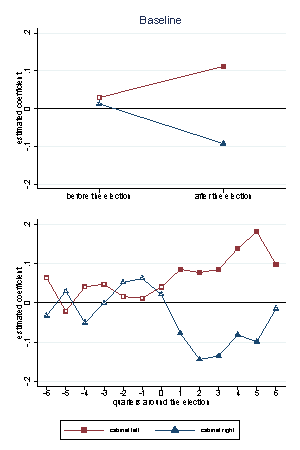
\includegraphics[width=\linewidth]{../results/applications/app_graphs_baseline.pdf}
		{\scriptsize Note: These figures show the time evolution of refugee inflows as estimated in fixed effects regression with a set of dummies for before and after the election or a set of dummies for different quarters before and after an election in a quarter t = 0. Significant coefficients are indicated by filled plot markers.\par}
	\end{minipage}
\end{figure}

\clearpage
\FloatBarrier
\begin{table}[!ht]\centering \footnotesize
\def\sym#1{\ifmmode^{#1}\else\(^{#1}\)\fi}
\caption{Coefficients Graph 1 - baseline}
\begin{tabular}{l*{3}{c}}
\hline\hline
                   &\multicolumn{1}{c}{(1)}&\multicolumn{1}{c}{(2)}&\multicolumn{1}{c}{(3)}\\
                    &\multicolumn{1}{c}{left}&\multicolumn{1}{c}{right}&\multicolumn{1}{c}{diff}\\
\hline
before              &      0.0291         &      0.0128         &      0.0163         \\
                    &    (0.0244)         &    (0.0234)         &    (0.0340)         \\
[0.5em]
after               &       0.112\sym{***}&     -0.0929\sym{***}&       0.205\sym{***}\\
                    &    (0.0215)         &    (0.0226)         &    (0.0314)         \\
\hline
Observations        &       23705         &       23705         &       23705         \\
\hline\hline
\multicolumn{4}{l}{\footnotesize Standard errors in parentheses}\\
\multicolumn{4}{l}{\footnotesize \sym{*} \(p<0.05\), \sym{**} \(p<0.01\), \sym{***} \(p<0.001\)}\\
\end{tabular}
\end{table}

\begin{table}[htbp]\centering
\def\sym#1{\ifmmode^{#1}\else\(^{#1}\)\fi}
\caption{Coefficients Graph 2}
\begin{tabular}{l*{2}{c}}
\hline\hline
                    &\multicolumn{1}{c}{(1)}&\multicolumn{1}{c}{(2)}\\
                    &\multicolumn{1}{c}{left}&\multicolumn{1}{c}{right}\\
\hline
 6 quarters before the election&      0.0555\sym{*}  &     -0.0244         \\
                    &    (0.0275)         &    (0.0365)         \\
[1em]
 5 quarters before the election&     -0.0294         &      0.0385         \\
                    &    (0.0295)         &    (0.0311)         \\
[1em]
 4 quarters before the election&      0.0333         &     -0.0422         \\
                    &    (0.0366)         &    (0.0385)         \\
[1em]
 3 quarters before the election&      0.0398         &     0.00650         \\
                    &    (0.0439)         &    (0.0302)         \\
[1em]
 2 quarters before the election&     0.00828         &      0.0600         \\
                    &    (0.0358)         &    (0.0385)         \\
[1em]
 1 quarters before the election&     0.00414         &      0.0701         \\
                    &    (0.0425)         &    (0.0363)         \\
[1em]
Quarter of the election&      0.0325         &      0.0293         \\
                    &    (0.0393)         &    (0.0374)         \\
[1em]
 1 quarters after the election&      0.0775\sym{*}  &     -0.0698         \\
                    &    (0.0373)         &    (0.0364)         \\
[1em]
 2 quarters after the election&      0.0697\sym{*}  &      -0.136\sym{***}\\
                    &    (0.0346)         &    (0.0338)         \\
[1em]
 3 quarters after the election&      0.0774\sym{*}  &      -0.127\sym{**} \\
                    &    (0.0339)         &    (0.0448)         \\
[1em]
 4 quarters after the election&       0.131\sym{***}&     -0.0733         \\
                    &    (0.0315)         &    (0.0384)         \\
[1em]
 5 quarters after the election&       0.173\sym{***}&     -0.0904\sym{**} \\
                    &    (0.0288)         &    (0.0350)         \\
[1em]
 6 quarters after the election&      0.0899\sym{***}&    -0.00688         \\
                    &    (0.0264)         &    (0.0296)         \\
\hline
Observations        &       23705         &       23705         \\
\hline\hline
\multicolumn{3}{l}{\footnotesize Standard errors in parentheses}\\
\multicolumn{3}{l}{\footnotesize \sym{*} \(p<0.05\), \sym{**} \(p<0.01\), \sym{***} \(p<0.001\)}\\
\end{tabular}
\end{table}



\clearpage
\FloatBarrier
\begin{figure}[!ht]
	\caption{First-time asylum applications per capita: predicted pattern - R1 to R6}
	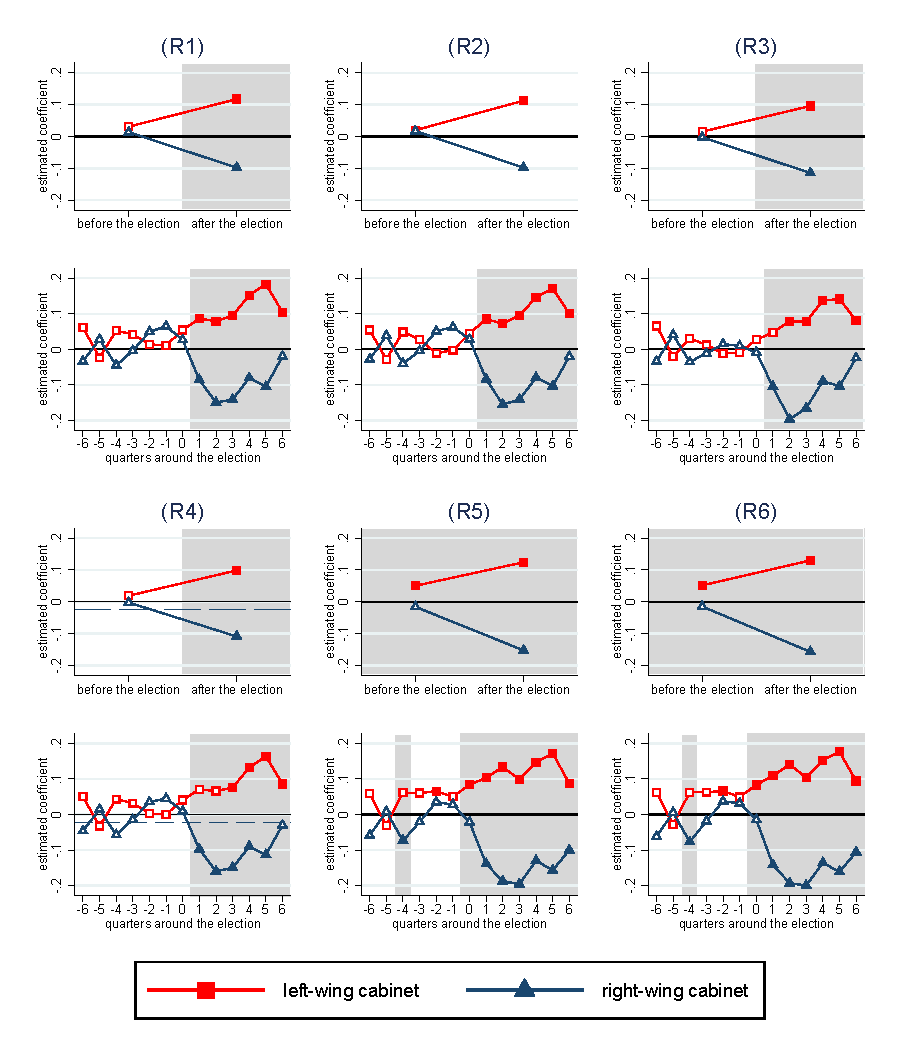
\includegraphics[width=1\textwidth]{../results/applications/app_graphs_R1-R6.pdf}
	\scriptsize{Note: These figures show the time evolution of refugee inflows as estimated in fixed effects regression
		with a set of dummies for before and after the election or a set of dummies for different quarters before and after an election in a quarter t = 0. Significant coefficients are indicated by filled plot markers. The dashed line in subfigure R4 shows the average inflow of asylum seekers under right-wing cabinets in periods outside the election period. Significance of the coefficients is reported for the distance to this average non-election period effect.}
\end{figure}

\clearpage
\FloatBarrier

\begin{table}[!ht]\centering \footnotesize
\def\sym#1{\ifmmode^{#1}\else\(^{#1}\)\fi}
\caption{Coefficients before after model - R1 - R2}
\begin{tabular}{l*{6}{c}}
\hline\hline
                    &\multicolumn{3}{c}{(R1)}&\multicolumn{3}{c}{(R2)}\\
                    &\multicolumn{1}{c}{left}&\multicolumn{1}{c}{right}&\multicolumn{1}{c}{diff}&\multicolumn{1}{c}{left}&\multicolumn{1}{c}{right}&\multicolumn{1}{c}{diff}\\
\hline
before              &      0.0295         &      0.0153         &      0.0143         &      0.0185         &      0.0189         &   -0.000336         \\
                    &    (0.0243)         &    (0.0233)         &    (0.0340)         &    (0.0250)         &    (0.0231)         &    (0.0346)         \\
[0.5em]
after               &       0.119\sym{***}&     -0.0948\sym{***}&       0.214\sym{***}&       0.114\sym{***}&     -0.0948\sym{***}&       0.209\sym{***}\\
                    &    (0.0226)         &    (0.0233)         &    (0.0332)         &    (0.0228)         &    (0.0230)         &    (0.0334)         \\
\hline
Observations        &       23705         &       23705         &       23705         &       23705         &       23705         &       23705         \\
\hline\hline
\multicolumn{7}{l}{ Standard errors in parentheses \sym{*} \(p<0.05\), \sym{**} \(p<0.01\), \sym{***} \(p<0.001\)}\\
\end{tabular}
\end{table}

\begin{table}[!ht]\centering \footnotesize
\def\sym#1{\ifmmode^{#1}\else\(^{#1}\)\fi}
\caption{Coefficients quarterly model - R1 - R2}
\begin{tabular}{l*{6}{c}}
\hline\hline
                    &\multicolumn{3}{c}{(R1)}&\multicolumn{3}{c}{(R2)}\\
                    &\multicolumn{1}{c}{left}&\multicolumn{1}{c}{right}&\multicolumn{1}{c}{diff}&\multicolumn{1}{c}{left}&\multicolumn{1}{c}{right}&\multicolumn{1}{c}{diff}\\
\hline
 6 quarters before the election&      0.0646         &     -0.0313         &      0.0959         &      0.0572         &     -0.0259         &      0.0830         \\
                    &    (0.0350)         &    (0.0410)         &    (0.0642)         &    (0.0362)         &    (0.0407)         &    (0.0658)         \\
[0.5em]
 5 quarters before the election&     -0.0231         &      0.0320         &     -0.0551         &     -0.0271         &      0.0430         &     -0.0701         \\
                    &    (0.0316)         &    (0.0343)         &    (0.0541)         &    (0.0315)         &    (0.0328)         &    (0.0529)         \\
[0.5em]
 4 quarters before the election&      0.0409         &     -0.0499         &      0.0908         &      0.0375         &     -0.0447         &      0.0822         \\
                    &    (0.0341)         &    (0.0369)         &    (0.0508)         &    (0.0345)         &    (0.0360)         &    (0.0506)         \\
[0.5em]
 3 quarters before the election&      0.0475         &    -0.00320         &      0.0507         &      0.0328         &    -0.00366         &      0.0364         \\
                    &    (0.0416)         &    (0.0303)         &    (0.0512)         &    (0.0429)         &    (0.0303)         &    (0.0521)         \\
[0.5em]
 2 quarters before the election&      0.0171         &      0.0540         &     -0.0370         &    -0.00771         &      0.0561         &     -0.0638         \\
                    &    (0.0338)         &    (0.0371)         &    (0.0463)         &    (0.0337)         &    (0.0370)         &    (0.0447)         \\
[0.5em]
 1 quarters before the election&      0.0126         &      0.0698\sym{*}  &     -0.0572         &    -0.00144         &      0.0674\sym{*}  &     -0.0689         \\
                    &    (0.0361)         &    (0.0343)         &    (0.0420)         &    (0.0362)         &    (0.0338)         &    (0.0420)         \\
[0.5em]
Quarter of the election&      0.0438         &      0.0263         &      0.0175         &      0.0342         &      0.0285         &     0.00571         \\
                    &    (0.0356)         &    (0.0387)         &    (0.0497)         &    (0.0362)         &    (0.0383)         &    (0.0522)         \\
[0.5em]
 1 quarters after the election&      0.0912\sym{*}  &     -0.0780\sym{*}  &       0.169\sym{***}&      0.0892\sym{*}  &     -0.0765\sym{*}  &       0.166\sym{***}\\
                    &    (0.0389)         &    (0.0320)         &    (0.0455)         &    (0.0396)         &    (0.0315)         &    (0.0460)         \\
[0.5em]
 2 quarters after the election&      0.0803\sym{**} &      -0.146\sym{***}&       0.226\sym{***}&      0.0735\sym{*}  &      -0.151\sym{***}&       0.225\sym{***}\\
                    &    (0.0304)         &    (0.0353)         &    (0.0427)         &    (0.0298)         &    (0.0361)         &    (0.0440)         \\
[0.5em]
 3 quarters after the election&      0.0947\sym{**} &      -0.138\sym{***}&       0.233\sym{***}&      0.0948\sym{**} &      -0.138\sym{***}&       0.233\sym{***}\\
                    &    (0.0331)         &    (0.0398)         &    (0.0553)         &    (0.0332)         &    (0.0376)         &    (0.0542)         \\
[0.5em]
 4 quarters after the election&       0.149\sym{***}&     -0.0835\sym{*}  &       0.232\sym{***}&       0.142\sym{***}&     -0.0823\sym{*}  &       0.225\sym{***}\\
                    &    (0.0290)         &    (0.0354)         &    (0.0477)         &    (0.0298)         &    (0.0363)         &    (0.0495)         \\
[0.5em]
 5 quarters after the election&       0.190\sym{***}&      -0.102\sym{**} &       0.292\sym{***}&       0.178\sym{***}&      -0.100\sym{**} &       0.278\sym{***}\\
                    &    (0.0297)         &    (0.0358)         &    (0.0472)         &    (0.0296)         &    (0.0356)         &    (0.0474)         \\
[0.5em]
 6 quarters after the election&       0.106\sym{**} &     -0.0164         &       0.122\sym{*}  &       0.101\sym{**} &     -0.0168         &       0.118\sym{*}  \\
                    &    (0.0322)         &    (0.0317)         &    (0.0492)         &    (0.0322)         &    (0.0311)         &    (0.0479)         \\
\hline
Observations        &       23705         &       23705         &       23705         &       23705         &       23705         &       23705         \\
\hline\hline
\multicolumn{7}{l}{ Standard errors in parentheses \sym{*} \(p<0.05\), \sym{**} \(p<0.01\), \sym{***} \(p<0.001\)}\\
\end{tabular}
\end{table}

\clearpage
\FloatBarrier
\begin{table}[!ht]\centering \footnotesize
\def\sym#1{\ifmmode^{#1}\else\(^{#1}\)\fi}
\caption{Coefficients before after model - R3 - R4}
\begin{tabular}{l*{6}{c}}
\hline\hline
                    &\multicolumn{3}{c}{(R3)}&\multicolumn{3}{c}{(R4)}\\
&\multicolumn{1}{c}{left}&\multicolumn{1}{c}{right}&\multicolumn{1}{c}{diff}&\multicolumn{1}{c}{left}&\multicolumn{1}{c}{right}&\multicolumn{1}{c}{diff}\\
\hline
before              &      0.0143         &    -0.00105         &      0.0153         &      0.0194         &      0.0223         &      0.0177         \\
                    &    (0.0239)         &    (0.0235)         &    (0.0335)         &    (0.0267)         &    (0.0223)         &    (0.0358)         \\
[0.5em]
after               &      0.0969\sym{***}&      -0.112\sym{***}&       0.209\sym{***}&       0.102\sym{***}&     -0.0831\sym{**} &       0.206\sym{***}\\
                    &    (0.0206)         &    (0.0229)         &    (0.0308)         &    (0.0229)         &    (0.0258)         &    (0.0325)         \\
\hline
Observations        &       23705         &       23705         &       23705         &       23705         &       23705         &       23705         \\
\hline\hline
\multicolumn{7}{l}{ Standard errors in parentheses \sym{*} \(p<0.05\), \sym{**} \(p<0.01\), \sym{***} \(p<0.001\)}\\
\end{tabular}
\end{table}

\begin{table}[!ht]\centering \footnotesize
\def\sym#1{\ifmmode^{#1}\else\(^{#1}\)\fi}
\caption{Coefficients quarterly model - R3 - R4}
\begin{tabular}{l*{6}{c}}
\hline\hline
                    &\multicolumn{1}{c}{(1)}&\multicolumn{1}{c}{(2)}&\multicolumn{1}{c}{(3)}&\multicolumn{1}{c}{(4)}&\multicolumn{1}{c}{(5)}&\multicolumn{1}{c}{(6)}\\
                    &\multicolumn{1}{c}{left2\_R3}&\multicolumn{1}{c}{right2\_R3}&\multicolumn{1}{c}{diff2\_R3}&\multicolumn{1}{c}{left2\_R4}&\multicolumn{1}{c}{right2\_R4}&\multicolumn{1}{c}{diff2\_R4}\\
\hline
 6 quarters before the election&      0.0652         &     -0.0339         &      0.0991         &      0.0501         &     -0.0248         &      0.0963         \\
                    &    (0.0338)         &    (0.0418)         &    (0.0639)         &    (0.0274)         &    (0.0365)         &    (0.0649)         \\
[1em]
 5 quarters before the election&     -0.0207         &      0.0405         &     -0.0611         &     -0.0324         &      0.0361         &     -0.0470         \\
                    &    (0.0316)         &    (0.0341)         &    (0.0538)         &    (0.0295)         &    (0.0311)         &    (0.0548)         \\
[1em]
 4 quarters before the election&      0.0303         &     -0.0357         &      0.0660         &      0.0433         &     -0.0354         &       0.100         \\
                    &    (0.0338)         &    (0.0364)         &    (0.0510)         &    (0.0365)         &    (0.0381)         &    (0.0522)         \\
[1em]
 3 quarters before the election&      0.0123         &     -0.0117         &      0.0240         &      0.0319         &     0.00719         &      0.0462         \\
                    &    (0.0409)         &    (0.0303)         &    (0.0517)         &    (0.0438)         &    (0.0302)         &    (0.0527)         \\
[1em]
 2 quarters before the election&     -0.0115         &      0.0147         &     -0.0263         &     0.00273         &      0.0566         &     -0.0324         \\
                    &    (0.0337)         &    (0.0367)         &    (0.0449)         &    (0.0361)         &    (0.0386)         &    (0.0467)         \\
[1em]
 1 quarters before the election&    -0.00969         &     0.00946         &     -0.0191         &    0.000695         &      0.0665         &     -0.0443         \\
                    &    (0.0362)         &    (0.0348)         &    (0.0418)         &    (0.0426)         &    (0.0364)         &    (0.0418)         \\
[1em]
Quarter of the election&      0.0271         &    -0.00884         &      0.0359         &      0.0410         &      0.0310         &      0.0315         \\
                    &    (0.0348)         &    (0.0383)         &    (0.0472)         &    (0.0390)         &    (0.0373)         &    (0.0510)         \\
[1em]
 1 quarters after the election&      0.0473         &      -0.105\sym{**} &       0.153\sym{***}&      0.0706         &     -0.0763\sym{*}  &       0.168\sym{***}\\
                    &    (0.0379)         &    (0.0329)         &    (0.0450)         &    (0.0371)         &    (0.0366)         &    (0.0468)         \\
[1em]
 2 quarters after the election&      0.0783\sym{**} &      -0.197\sym{***}&       0.275\sym{***}&      0.0660         &      -0.138\sym{***}&       0.225\sym{***}\\
                    &    (0.0290)         &    (0.0352)         &    (0.0418)         &    (0.0346)         &    (0.0339)         &    (0.0433)         \\
[1em]
 3 quarters after the election&      0.0777\sym{*}  &      -0.165\sym{***}&       0.243\sym{***}&      0.0754\sym{*}  &      -0.128\sym{**} &       0.225\sym{***}\\
                    &    (0.0318)         &    (0.0400)         &    (0.0536)         &    (0.0339)         &    (0.0449)         &    (0.0544)         \\
[1em]
 4 quarters after the election&       0.137\sym{***}&     -0.0895\sym{**} &       0.226\sym{***}&       0.132\sym{***}&     -0.0684         &       0.222\sym{***}\\
                    &    (0.0272)         &    (0.0345)         &    (0.0450)         &    (0.0314)         &    (0.0384)         &    (0.0464)         \\
[1em]
 5 quarters after the election&       0.142\sym{***}&      -0.104\sym{**} &       0.246\sym{***}&       0.164\sym{***}&     -0.0919\sym{**} &       0.277\sym{***}\\
                    &    (0.0266)         &    (0.0357)         &    (0.0452)         &    (0.0286)         &    (0.0350)         &    (0.0466)         \\
[1em]
 6 quarters after the election&      0.0802\sym{**} &     -0.0245         &       0.105\sym{*}  &      0.0861\sym{***}&    -0.00824         &       0.116\sym{*}  \\
                    &    (0.0293)         &    (0.0303)         &    (0.0461)         &    (0.0262)         &    (0.0296)         &    (0.0476)         \\
\hline
Observations        &       23705         &       23705         &       23705         &       23705         &       23705         &       23705         \\
\hline\hline
\multicolumn{7}{l}{\footnotesize Standard errors in parentheses}\\
\multicolumn{7}{l}{\footnotesize \sym{*} \(p<0.05\), \sym{**} \(p<0.01\), \sym{***} \(p<0.001\)}\\
\end{tabular}
\end{table}

\clearpage
\FloatBarrier
\begin{table}[!ht]\centering \footnotesize
\def\sym#1{\ifmmode^{#1}\else\(^{#1}\)\fi}
\caption{Coefficients before after model R5 - R6}
\begin{tabular}{l*{6}{c}}
\hline\hline
                    &\multicolumn{3}{c}{(R5)}&\multicolumn{3}{c}{(R6)}\\
&\multicolumn{1}{c}{left}&\multicolumn{1}{c}{right}&\multicolumn{1}{c}{diff}&\multicolumn{1}{c}{left}&\multicolumn{1}{c}{right}&\multicolumn{1}{c}{diff}\\
\hline
before              &      0.0484\sym{*}  &     -0.0134         &      0.0619         &      0.0494\sym{*}  &     -0.0123         &      0.0617\sym{*}  \\
                    &    (0.0235)         &    (0.0232)         &    (0.0320)         &    (0.0229)         &    (0.0230)         &    (0.0305)         \\
[0.5em]
after               &       0.126\sym{***}&      -0.148\sym{***}&       0.274\sym{***}&       0.131\sym{***}&      -0.153\sym{***}&       0.284\sym{***}\\
                    &    (0.0217)         &    (0.0237)         &    (0.0328)         &    (0.0229)         &    (0.0247)         &    (0.0359)         \\
\hline
Observations        &       23705         &       23705         &       23705         &       23705         &       23705         &       23705         \\
\hline\hline
\multicolumn{7}{l}{ Standard errors in parentheses \sym{*} \(p<0.05\), \sym{**} \(p<0.01\), \sym{***} \(p<0.001\)}\\
\end{tabular}
\end{table}

\begin{table}[!ht]\centering \footnotesize
\def\sym#1{\ifmmode^{#1}\else\(^{#1}\)\fi}
\caption{Coefficients quarterly model R5 - R6}
\begin{tabular}{l*{6}{c}}
\hline\hline
                     &\multicolumn{3}{c}{(R5)}&\multicolumn{3}{c}{(R6)}\\
 &\multicolumn{1}{c}{left}&\multicolumn{1}{c}{right}&\multicolumn{1}{c}{diff}&\multicolumn{1}{c}{left}&\multicolumn{1}{c}{right}&\multicolumn{1}{c}{diff}\\
 \hline
 6 quarters before the election&      0.0624         &     -0.0554         &       0.118         &      0.0658         &     -0.0580         &       0.124         \\
                    &    (0.0338)         &    (0.0414)         &    (0.0637)         &    (0.0348)         &    (0.0407)         &    (0.0638)         \\
[0.5em]
 5 quarters before the election&     -0.0301         &      0.0137         &     -0.0438         &     -0.0269         &      0.0115         &     -0.0385         \\
                    &    (0.0315)         &    (0.0346)         &    (0.0537)         &    (0.0311)         &    (0.0335)         &    (0.0517)         \\
[0.5em]
 4 quarters before the election&      0.0481         &     -0.0786\sym{*}  &       0.127\sym{*}  &      0.0481         &     -0.0819\sym{*}  &       0.130\sym{**} \\
                    &    (0.0339)         &    (0.0366)         &    (0.0497)         &    (0.0335)         &    (0.0358)         &    (0.0480)         \\
[0.5em]
 3 quarters before the election&      0.0667         &     -0.0195         &      0.0862         &      0.0692         &     -0.0170         &      0.0862         \\
                    &    (0.0407)         &    (0.0302)         &    (0.0497)         &    (0.0406)         &    (0.0296)         &    (0.0474)         \\
[0.5em]
 2 quarters before the election&      0.0693\sym{*}  &      0.0414         &      0.0279         &      0.0697\sym{*}  &      0.0436         &      0.0261         \\
                    &    (0.0323)         &    (0.0376)         &    (0.0437)         &    (0.0322)         &    (0.0380)         &    (0.0441)         \\
[0.5em]
 1 quarters before the election&      0.0513         &      0.0343         &      0.0171         &      0.0503         &      0.0382         &      0.0121         \\
                    &    (0.0354)         &    (0.0336)         &    (0.0389)         &    (0.0339)         &    (0.0336)         &    (0.0367)         \\
[0.5em]
Quarter of the election&      0.0712\sym{*}  &     -0.0204         &      0.0916\sym{*}  &      0.0703\sym{*}  &     -0.0140         &      0.0844         \\
                    &    (0.0347)         &    (0.0381)         &    (0.0463)         &    (0.0339)         &    (0.0376)         &    (0.0441)         \\
[0.5em]
 1 quarters after the election&       0.108\sym{**} &      -0.128\sym{***}&       0.237\sym{***}&       0.115\sym{**} &      -0.131\sym{***}&       0.246\sym{***}\\
                    &    (0.0387)         &    (0.0332)         &    (0.0457)         &    (0.0384)         &    (0.0336)         &    (0.0463)         \\
[0.5em]
 2 quarters after the election&       0.135\sym{***}&      -0.182\sym{***}&       0.318\sym{***}&       0.141\sym{***}&      -0.187\sym{***}&       0.329\sym{***}\\
                    &    (0.0320)         &    (0.0355)         &    (0.0445)         &    (0.0330)         &    (0.0361)         &    (0.0467)         \\
[0.5em]
 3 quarters after the election&      0.0985\sym{**} &      -0.191\sym{***}&       0.290\sym{***}&       0.104\sym{**} &      -0.195\sym{***}&       0.299\sym{***}\\
                    &    (0.0325)         &    (0.0395)         &    (0.0546)         &    (0.0332)         &    (0.0401)         &    (0.0562)         \\
[0.5em]
 4 quarters after the election&       0.143\sym{***}&      -0.133\sym{***}&       0.276\sym{***}&       0.148\sym{***}&      -0.138\sym{***}&       0.287\sym{***}\\
                    &    (0.0281)         &    (0.0354)         &    (0.0473)         &    (0.0293)         &    (0.0369)         &    (0.0505)         \\
[0.5em]
 5 quarters after the election&       0.180\sym{***}&      -0.152\sym{***}&       0.332\sym{***}&       0.185\sym{***}&      -0.157\sym{***}&       0.341\sym{***}\\
                    &    (0.0278)         &    (0.0365)         &    (0.0473)         &    (0.0290)         &    (0.0375)         &    (0.0501)         \\
[0.5em]
 6 quarters after the election&      0.0894\sym{**} &     -0.0954\sym{**} &       0.185\sym{***}&      0.0958\sym{**} &      -0.100\sym{**} &       0.196\sym{***}\\
                    &    (0.0300)         &    (0.0308)         &    (0.0467)         &    (0.0313)         &    (0.0319)         &    (0.0498)         \\
\hline
Observations        &       23705         &       23705         &       23705         &       23705         &       23705         &       23705         \\
\hline\hline
\multicolumn{7}{l}{ Standard errors in parentheses \sym{*} \(p<0.05\), \sym{**} \(p<0.01\), \sym{***} \(p<0.001\)}\\
\end{tabular}
\end{table}


\clearpage
\FloatBarrier
\begin{table}[htbp]\centering \footnotesize
\def\sym#1{\ifmmode^{#1}\else\(^{#1}\)\fi}
\caption{Determinants of first-time asylum applications per capita - R7 - R12}
\begin{tabular}{l*{6}{c}}
\hline\hline
	&\multicolumn{1}{c}{(1)}     &\multicolumn{1}{c}{(2)}       &\multicolumn{1}{c}{(3)}       &\multicolumn{1}{c}{(4)}    	&\multicolumn{1}{c}{(5)}  	&\multicolumn{1}{c}{(6)}   \\
                    &\multicolumn{1}{c}{R7}         &\multicolumn{1}{c}{R8}         &\multicolumn{1}{c}{R9}         &\multicolumn{1}{c}{R10}         &\multicolumn{1}{c}{R11}         &\multicolumn{1}{c}{R12}         \\
\hline
Political Terror Scale	&       0.400\sym{***}& 0.337\sym{***}    &       0.409\sym{***}&       0.400\sym{***}&       0.400\sym{***}&       0.404\sym{***}\\
                    	&    (0.0696)         &     (0.0616)                  &    (0.0696)         &    (0.0697)         &    (0.0450)         &    (0.0706)         \\
[0,5em]
Civic Liberty (FHI) 	&       0.142         &        0.129              &       0.176         &       0.175         &       0.175\sym{**} &       0.170         \\
                    	&     (0.127)         &        (0.123)             &     (0.129)         &     (0.131)         &    (0.0611)         &     (0.134)         \\
[0,5em]
Political Rights (FHI)	&      0.0633         &       0.0564                &      0.0450         &      0.0487         &      0.0487         &      0.0476         \\
                    	&    (0.0712)         &          (0.0670)           &    (0.0751)         &    (0.0752)         &    (0.0479)         &    (0.0758)         \\
[0,5em]
Quarterly civil war 	&       0.192\sym{***}&     0.160\sym{***}          &    0.126\sym{***}                 &       0.188\sym{***}&       0.188\sym{***}&       0.186\sym{***}\\
battle death (000s)     &    (0.0224)         &  (0.0221)                   &     (0.0139)                 &    (0.0234)         &    (0.0265)         &    (0.0236)         \\
[0,5em]
Log origin country 		&      -0.636\sym{***}&   -0.693\sym{***}                  &      -0.654\sym{***}&      -0.661\sym{***}&      -0.661\sym{***}&      -0.651\sym{***}\\
real GDP per capita     &     (0.158)         &     (0.149)                 &     (0.167)         &     (0.163)         &     (0.105)         &     (0.163)         \\
[0,5em]
Log destination country &      -1.484\sym{**} &      -1.447\sym{**} &      -1.464\sym{**} &      -1.470\sym{**} &      -1.470\sym{*}  &      -1.483\sym{**} \\
real GDP per capita     &     (0.443)         &     (0.439)         &     (0.440)         &     (0.440)         &     (0.608)         &     (0.443)         \\
[0,5em]
Quarterly unemployment &     -0.0714\sym{***}&     -0.0740\sym{***}&     -0.0744\sym{***}&     -0.0745\sym{***}&     -0.0745\sym{***}&     -0.0714\sym{***}\\
rate at destination    &    (0.0108)         &    (0.0108)         &    (0.0108)         &    (0.0108)         &    (0.0112)         &    (0.0108)         \\
[0,5em]
Years after 2007          &                     &                     &                     &       0.190         &                     &                     \\
                    &                     &                     &                     &     (0.183)         &                     &                     \\
[0,5em]
Cabinet position left * &      0.0357         &      0.0290         &      0.0288         &      0.0291         &      0.0291         &      0.0248         \\
Before the election                    &    (0.0245)         &    (0.0245)         &    (0.0244)         &    (0.0244)         &    (0.0301)         &    (0.0240)         \\
[0,5em]
Cabinet position left * &       0.115\sym{***}&       0.112\sym{***}&       0.112\sym{***}&       0.112\sym{***}&       0.112\sym{***}&      0.0993\sym{***}\\
After the election                    &    (0.0215)         &    (0.0216)         &    (0.0215)         &    (0.0215)         &    (0.0286)         &    (0.0220)         \\
[0,5em]
Cabinet position right * &     0.00861         &      0.0120         &      0.0128         &      0.0128         &      0.0128         &      0.0135         \\
Before the election                    &    (0.0234)         &    (0.0234)         &    (0.0235)         &    (0.0234)         &    (0.0302)         &    (0.0238)         \\
[0,5em]
Cabinet position right * &     -0.0945\sym{***}&     -0.0945\sym{***}&     -0.0923\sym{***}&     -0.0929\sym{***}&     -0.0929\sym{**} &     -0.0913\sym{***}\\
After the election                    &    (0.0225)         &    (0.0223)         &    (0.0227)         &    (0.0226)         &    (0.0303)         &    (0.0261)         \\
\hline
Observations        &       23705         &       23705         &       23705         &       23705         &       23705         &       23239         \\
Adjusted \(R^{2}\)  &       0.182         &       0.168         &       0.177         &       0.176         &       0.176         &       0.175         \\
Fixed Effects       &       D x O         &       D x O         &       D x O         &       D x O         &       D x O         &       D x O         \\
Destination dummies &          No         &          No         &          No         &          No         &          No         &          No         \\
Quarter-Year dummies&         Yes         &         Yes         &         Yes         &         Yes         &         Yes         &         Yes         \\
\hline\hline
\multicolumn{7}{l}{Standard errors in parentheses \sym{*} \(p<0.05\), \sym{**} \(p<0.01\), \sym{***} \(p<0.001\)}\\
\end{tabular}
\end{table}


\clearpage
\FloatBarrier
\begin{figure}[!ht]
	\caption{First-time asylum applications per capita: predicted pattern - R7 to R12}
	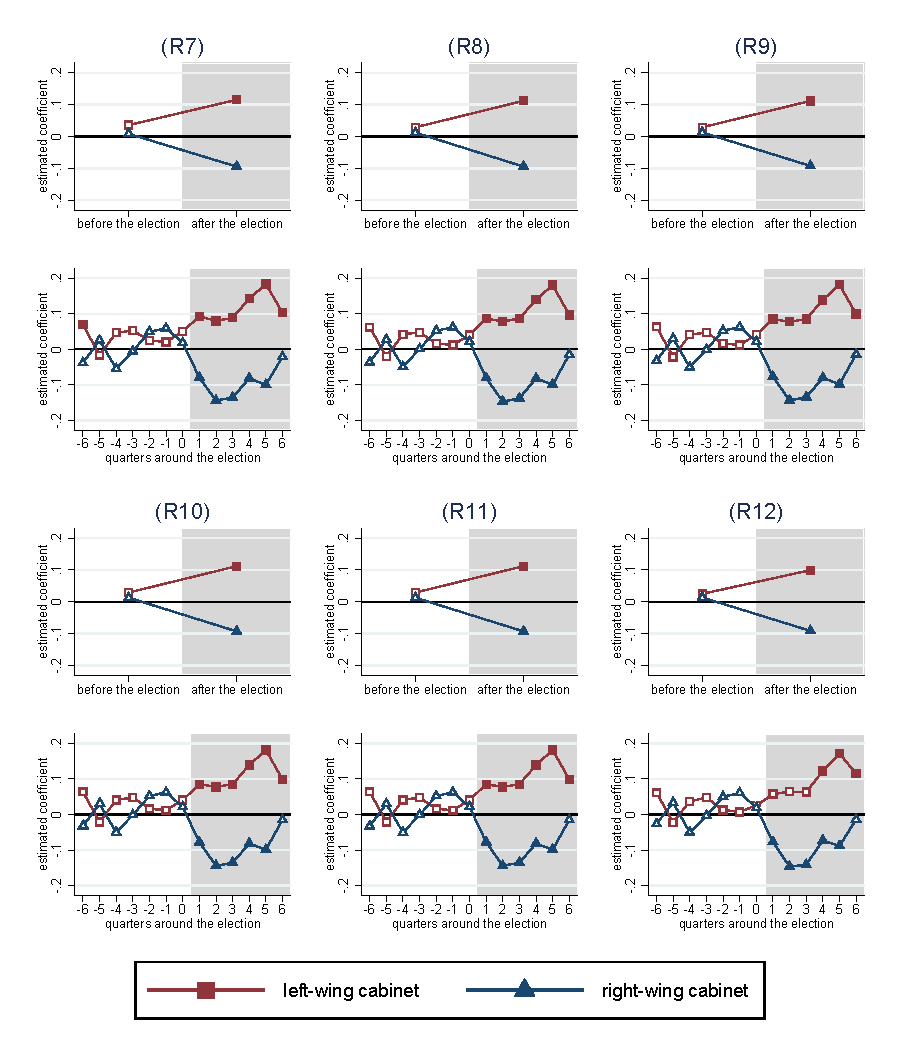
\includegraphics[width=1\textwidth]{../results/applications/app_graphs_R7-R12.pdf}
	\scriptsize{Note: These figures show the time evolution of refugee inflows as estimated in fixed effects regression
		with a set of dummies for before and after the election or a set of dummies for different quarters before and after an election in a quarter t = 0. Significant coefficients are indicated by filled plot markers.}
\end{figure}

\clearpage
\FloatBarrier

\begin{table}[!ht]\centering \footnotesize
\def\sym#1{\ifmmode^{#1}\else\(^{#1}\)\fi}
\caption{Coefficients before after model - R7 - R8}
\begin{tabular}{l*{6}{c}}
\hline\hline
                    &\multicolumn{1}{c}{(1)}&\multicolumn{1}{c}{(2)}&\multicolumn{1}{c}{(3)}&\multicolumn{1}{c}{(4)}&\multicolumn{1}{c}{(5)}&\multicolumn{1}{c}{(6)}\\
                    &\multicolumn{1}{c}{left1\_R7}&\multicolumn{1}{c}{right1\_R7}&\multicolumn{1}{c}{diff1\_R7}&\multicolumn{1}{c}{left1\_R8}&\multicolumn{1}{c}{right1\_R8}&\multicolumn{1}{c}{diff1\_R8}\\
\hline
before              &      0.0371         &     0.00683         &      0.0302         &      0.0304         &      0.0101         &      0.0203         \\
                    &    (0.0246)         &    (0.0234)         &    (0.0343)         &    (0.0246)         &    (0.0235)         &    (0.0341)         \\
[1em]
after               &       0.114\sym{***}&     -0.0977\sym{***}&       0.211\sym{***}&       0.110\sym{***}&     -0.0977\sym{***}&       0.208\sym{***}\\
                    &    (0.0213)         &    (0.0226)         &    (0.0314)         &    (0.0215)         &    (0.0224)         &    (0.0312)         \\
\hline
Observations        &       23705         &       23705         &       23705         &       23705         &       23705         &       23705         \\
\hline\hline
\multicolumn{7}{l}{\footnotesize Standard errors in parentheses}\\
\multicolumn{7}{l}{\footnotesize \sym{*} \(p<0.05\), \sym{**} \(p<0.01\), \sym{***} \(p<0.001\)}\\
\end{tabular}
\end{table}

\begin{table}[!ht]\centering \footnotesize
\def\sym#1{\ifmmode^{#1}\else\(^{#1}\)\fi}
\caption{Coefficients quarterly model - R7 - R8}
\begin{tabular}{l*{6}{c}}
\hline\hline
                    &\multicolumn{1}{c}{(1)}&\multicolumn{1}{c}{(2)}&\multicolumn{1}{c}{(3)}&\multicolumn{1}{c}{(4)}&\multicolumn{1}{c}{(5)}&\multicolumn{1}{c}{(6)}\\
                    &\multicolumn{1}{c}{left2\_R7}&\multicolumn{1}{c}{right2\_R7}&\multicolumn{1}{c}{diff2\_R7}&\multicolumn{1}{c}{left2\_R8}&\multicolumn{1}{c}{right2\_R8}&\multicolumn{1}{c}{diff2\_R8}\\
\hline
 6 quarters before the election&      0.0660         &     -0.0407         &       0.107         &      0.0588         &     -0.0392         &      0.0980         \\
                    &    (0.0338)         &    (0.0417)         &    (0.0638)         &    (0.0342)         &    (0.0413)         &    (0.0637)         \\
[1em]
 5 quarters before the election&     -0.0177         &      0.0211         &     -0.0388         &     -0.0215         &      0.0231         &     -0.0446         \\
                    &    (0.0314)         &    (0.0347)         &    (0.0539)         &    (0.0318)         &    (0.0347)         &    (0.0544)         \\
[1em]
 4 quarters before the election&      0.0579         &     -0.0500         &       0.108\sym{*}  &      0.0540         &     -0.0450         &      0.0990         \\
                    &    (0.0342)         &    (0.0366)         &    (0.0513)         &    (0.0340)         &    (0.0364)         &    (0.0512)         \\
[1em]
 3 quarters before the election&      0.0472         &    -0.00654         &      0.0538         &      0.0413         &   -0.000311         &      0.0417         \\
                    &    (0.0414)         &    (0.0299)         &    (0.0517)         &    (0.0414)         &    (0.0302)         &    (0.0514)         \\
[1em]
 2 quarters before the election&      0.0209         &      0.0442         &     -0.0233         &      0.0130         &      0.0472         &     -0.0342         \\
                    &    (0.0339)         &    (0.0373)         &    (0.0457)         &    (0.0338)         &    (0.0369)         &    (0.0452)         \\
[1em]
 1 quarters before the election&      0.0192         &      0.0535         &     -0.0344         &      0.0104         &      0.0562         &     -0.0458         \\
                    &    (0.0366)         &    (0.0340)         &    (0.0415)         &    (0.0365)         &    (0.0341)         &    (0.0410)         \\
[1em]
Quarter of the election&      0.0600         &      0.0180         &      0.0419         &      0.0511         &      0.0210         &      0.0301         \\
                    &    (0.0361)         &    (0.0383)         &    (0.0499)         &    (0.0362)         &    (0.0384)         &    (0.0504)         \\
[1em]
 1 quarters after the election&      0.0879\sym{*}  &     -0.0876\sym{**} &       0.176\sym{***}&      0.0816\sym{*}  &     -0.0892\sym{**} &       0.171\sym{***}\\
                    &    (0.0387)         &    (0.0325)         &    (0.0451)         &    (0.0387)         &    (0.0325)         &    (0.0454)         \\
[1em]
 2 quarters after the election&      0.0780\sym{**} &      -0.148\sym{***}&       0.226\sym{***}&      0.0760\sym{*}  &      -0.151\sym{***}&       0.227\sym{***}\\
                    &    (0.0302)         &    (0.0352)         &    (0.0422)         &    (0.0308)         &    (0.0350)         &    (0.0420)         \\
[1em]
 3 quarters after the election&      0.0883\sym{**} &      -0.139\sym{***}&       0.227\sym{***}&      0.0865\sym{**} &      -0.141\sym{***}&       0.228\sym{***}\\
                    &    (0.0324)         &    (0.0392)         &    (0.0542)         &    (0.0322)         &    (0.0395)         &    (0.0541)         \\
[1em]
 4 quarters after the election&       0.146\sym{***}&     -0.0787\sym{*}  &       0.224\sym{***}&       0.142\sym{***}&     -0.0792\sym{*}  &       0.222\sym{***}\\
                    &    (0.0278)         &    (0.0345)         &    (0.0459)         &    (0.0282)         &    (0.0341)         &    (0.0458)         \\
[1em]
 5 quarters after the election&       0.176\sym{***}&      -0.103\sym{**} &       0.280\sym{***}&       0.174\sym{***}&      -0.103\sym{**} &       0.277\sym{***}\\
                    &    (0.0274)         &    (0.0357)         &    (0.0464)         &    (0.0279)         &    (0.0352)         &    (0.0463)         \\
[1em]
 6 quarters after the election&       0.101\sym{***}&     -0.0241         &       0.125\sym{**} &      0.0946\sym{**} &     -0.0179         &       0.113\sym{*}  \\
                    &    (0.0299)         &    (0.0304)         &    (0.0469)         &    (0.0304)         &    (0.0301)         &    (0.0471)         \\
\hline
Observations        &       23705         &       23705         &       23705         &       23705         &       23705         &       23705         \\
\hline\hline
\multicolumn{7}{l}{\footnotesize Standard errors in parentheses}\\
\multicolumn{7}{l}{\footnotesize \sym{*} \(p<0.05\), \sym{**} \(p<0.01\), \sym{***} \(p<0.001\)}\\
\end{tabular}
\end{table}

\clearpage
\FloatBarrier
\begin{table}[!ht]\centering \footnotesize
\def\sym#1{\ifmmode^{#1}\else\(^{#1}\)\fi}
\caption{Coefficients before after model - R9 - R10}
\begin{tabular}{l*{6}{c}}
\hline\hline
                    &\multicolumn{1}{c}{(1)}&\multicolumn{1}{c}{(2)}&\multicolumn{1}{c}{(3)}&\multicolumn{1}{c}{(4)}&\multicolumn{1}{c}{(5)}&\multicolumn{1}{c}{(6)}\\
                    &\multicolumn{1}{c}{left1\_R9}&\multicolumn{1}{c}{right1\_R9}&\multicolumn{1}{c}{diff1\_R9}&\multicolumn{1}{c}{left1\_R10}&\multicolumn{1}{c}{right1\_R10}&\multicolumn{1}{c}{diff1\_R10}\\
\hline
before              &      0.0302         &      0.0110         &      0.0192         &      0.0304         &      0.0109         &      0.0195         \\
                    &    (0.0245)         &    (0.0235)         &    (0.0342)         &    (0.0245)         &    (0.0235)         &    (0.0342)         \\
[1em]
after               &       0.110\sym{***}&     -0.0956\sym{***}&       0.206\sym{***}&       0.110\sym{***}&     -0.0962\sym{***}&       0.206\sym{***}\\
                    &    (0.0213)         &    (0.0227)         &    (0.0315)         &    (0.0213)         &    (0.0226)         &    (0.0314)         \\
\hline
Observations        &       23705         &       23705         &       23705         &       23705         &       23705         &       23705         \\
\hline\hline
\multicolumn{7}{l}{\footnotesize Standard errors in parentheses}\\
\multicolumn{7}{l}{\footnotesize \sym{*} \(p<0.05\), \sym{**} \(p<0.01\), \sym{***} \(p<0.001\)}\\
\end{tabular}
\end{table}

\begin{table}[!ht]\centering \footnotesize
\def\sym#1{\ifmmode^{#1}\else\(^{#1}\)\fi}
\caption{Coefficients quarterly model - R9 - R10}
\begin{tabular}{l*{6}{c}}
\hline\hline
                    &\multicolumn{3}{c}{(R9)}&\multicolumn{3}{c}{(R10)}\\
&\multicolumn{1}{c}{left}&\multicolumn{1}{c}{right}&\multicolumn{1}{c}{diff}&\multicolumn{1}{c}{left}&\multicolumn{1}{c}{right}&\multicolumn{1}{c}{diff}\\

\hline
 6 quarters before the election&      0.0630         &     -0.0325         &      0.0955         &      0.0638         &     -0.0326         &      0.0964         \\
                    &    (0.0342)         &    (0.0414)         &    (0.0640)         &    (0.0340)         &    (0.0415)         &    (0.0639)         \\
[0.5em]
 5 quarters before the election&     -0.0218         &      0.0301         &     -0.0520         &     -0.0213         &      0.0301         &     -0.0513         \\
                    &    (0.0314)         &    (0.0346)         &    (0.0538)         &    (0.0313)         &    (0.0346)         &    (0.0537)         \\
[0.5em]
 4 quarters before the election&      0.0407         &     -0.0504         &      0.0911         &      0.0411         &     -0.0504         &      0.0916         \\
                    &    (0.0340)         &    (0.0371)         &    (0.0510)         &    (0.0341)         &    (0.0370)         &    (0.0509)         \\
[0.5em]
 3 quarters before the election&      0.0473         &    -0.00110         &      0.0484         &      0.0477         &    -0.00112         &      0.0488         \\
                    &    (0.0414)         &    (0.0299)         &    (0.0513)         &    (0.0414)         &    (0.0299)         &    (0.0513)         \\
[0.5em]
 2 quarters before the election&      0.0160         &      0.0523         &     -0.0363         &      0.0161         &      0.0522         &     -0.0361         \\
                    &    (0.0336)         &    (0.0373)         &    (0.0454)         &    (0.0336)         &    (0.0373)         &    (0.0454)         \\
[0.5em]
 1 quarters before the election&      0.0123         &      0.0624         &     -0.0501         &      0.0122         &      0.0623         &     -0.0501         \\
                    &    (0.0363)         &    (0.0342)         &    (0.0412)         &    (0.0363)         &    (0.0342)         &    (0.0413)         \\
[0.5em]
Quarter of the election&      0.0408         &      0.0215         &      0.0193         &      0.0406         &      0.0215         &      0.0191         \\
                    &    (0.0361)         &    (0.0385)         &    (0.0497)         &    (0.0362)         &    (0.0385)         &    (0.0497)         \\
[0.5em]
 1 quarters after the election&      0.0852\sym{*}  &     -0.0775\sym{*}  &       0.163\sym{***}&      0.0853\sym{*}  &     -0.0777\sym{*}  &       0.163\sym{***}\\
                    &    (0.0390)         &    (0.0324)         &    (0.0452)         &    (0.0390)         &    (0.0324)         &    (0.0452)         \\
[0.5em]
 2 quarters after the election&      0.0771\sym{*}  &      -0.144\sym{***}&       0.221\sym{***}&      0.0775\sym{*}  &      -0.144\sym{***}&       0.222\sym{***}\\
                    &    (0.0304)         &    (0.0354)         &    (0.0423)         &    (0.0303)         &    (0.0353)         &    (0.0422)         \\
[0.5em]
 3 quarters after the election&      0.0849\sym{**} &      -0.135\sym{***}&       0.220\sym{***}&      0.0852\sym{**} &      -0.136\sym{***}&       0.221\sym{***}\\
                    &    (0.0324)         &    (0.0390)         &    (0.0537)         &    (0.0324)         &    (0.0391)         &    (0.0539)         \\
[0.5em]
 4 quarters after the election&       0.139\sym{***}&     -0.0805\sym{*}  &       0.219\sym{***}&       0.139\sym{***}&     -0.0814\sym{*}  &       0.220\sym{***}\\
                    &    (0.0278)         &    (0.0347)         &    (0.0461)         &    (0.0278)         &    (0.0345)         &    (0.0458)         \\
[0.5em]
 5 quarters after the election&       0.182\sym{***}&     -0.0982\sym{**} &       0.280\sym{***}&       0.181\sym{***}&     -0.0990\sym{**} &       0.280\sym{***}\\
                    &    (0.0276)         &    (0.0358)         &    (0.0468)         &    (0.0277)         &    (0.0356)         &    (0.0466)         \\
[0.5em]
 6 quarters after the election&      0.0989\sym{***}&     -0.0143         &       0.113\sym{*}  &      0.0985\sym{**} &     -0.0149         &       0.113\sym{*}  \\
                    &    (0.0300)         &    (0.0303)         &    (0.0467)         &    (0.0301)         &    (0.0302)         &    (0.0467)         \\
\hline
Observations        &       23705         &       23705         &       23705         &       23705         &       23705         &       23705         \\
\hline\hline
\multicolumn{7}{l}{ Standard errors in parentheses \sym{*} \(p<0.05\), \sym{**} \(p<0.01\), \sym{***} \(p<0.001\)}\\
\end{tabular}
\end{table}

\clearpage
\FloatBarrier
\begin{table}[!ht]\centering \footnotesize
\def\sym#1{\ifmmode^{#1}\else\(^{#1}\)\fi}
\caption{Coefficients before after model R11 - R12}
\begin{tabular}{l*{6}{c}}
\hline\hline
                    &\multicolumn{3}{c}{(R11)}&\multicolumn{3}{c}{(R12)}\\
&\multicolumn{1}{c}{left}&\multicolumn{1}{c}{right}&\multicolumn{1}{c}{diff}&\multicolumn{1}{c}{left}&\multicolumn{1}{c}{right}&\multicolumn{1}{c}{diff}\\
\hline
before              &      0.0291         &      0.0128         &      0.0163         &      0.0248         &      0.0135         &      0.0113         \\
                    &    (0.0301)         &    (0.0302)         &    (0.0473)         &    (0.0240)         &    (0.0238)         &    (0.0335)         \\
[0.5em]
after               &       0.112\sym{***}&     -0.0929\sym{**} &       0.205\sym{***}&      0.0993\sym{***}&     -0.0913\sym{***}&       0.191\sym{***}\\
                    &    (0.0286)         &    (0.0303)         &    (0.0436)         &    (0.0220)         &    (0.0261)         &    (0.0332)         \\
\hline
Observations        &       23705         &       23705         &       23705         &       23239         &       23239         &       23239         \\
\hline\hline
\multicolumn{7}{l}{ Standard errors in parentheses \sym{*} \(p<0.05\), \sym{**} \(p<0.01\), \sym{***} \(p<0.001\)}\\
\end{tabular}
\end{table}

\begin{table}[!ht]\centering \footnotesize
\def\sym#1{\ifmmode^{#1}\else\(^{#1}\)\fi}
\caption{Coefficients quarterly model R11 - R12}
\begin{tabular}{l*{6}{c}}
\hline\hline
                    &\multicolumn{1}{c}{(1)}&\multicolumn{1}{c}{(2)}&\multicolumn{1}{c}{(3)}&\multicolumn{1}{c}{(4)}&\multicolumn{1}{c}{(5)}&\multicolumn{1}{c}{(6)}\\
                    &\multicolumn{1}{c}{left2\_R11}&\multicolumn{1}{c}{right2\_R11}&\multicolumn{1}{c}{diff2\_R11}&\multicolumn{1}{c}{left2\_R12}&\multicolumn{1}{c}{right2\_R12}&\multicolumn{1}{c}{diff2\_R12}\\
\hline
 6 quarters before the election&      0.0605         &     -0.0350         &      0.0955         &      0.0578         &     -0.0297         &      0.0875         \\
                    &    (0.0395)         &    (0.0407)         &    (0.0629)         &    (0.0322)         &    (0.0417)         &    (0.0626)         \\
[1em]
 5 quarters before the election&     -0.0222         &      0.0256         &     -0.0479         &     -0.0227         &      0.0288         &     -0.0515         \\
                    &    (0.0386)         &    (0.0404)         &    (0.0632)         &    (0.0306)         &    (0.0346)         &    (0.0533)         \\
[1em]
 4 quarters before the election&      0.0530         &     -0.0457         &      0.0987         &      0.0488         &     -0.0456         &      0.0945         \\
                    &    (0.0433)         &    (0.0425)         &    (0.0625)         &    (0.0340)         &    (0.0364)         &    (0.0505)         \\
[1em]
 3 quarters before the election&      0.0418         &    -0.00232         &      0.0442         &      0.0417         &    -0.00478         &      0.0464         \\
                    &    (0.0491)         &    (0.0463)         &    (0.0686)         &    (0.0420)         &    (0.0305)         &    (0.0524)         \\
[1em]
 2 quarters before the election&      0.0125         &      0.0468         &     -0.0343         &     0.00869         &      0.0443         &     -0.0356         \\
                    &    (0.0434)         &    (0.0454)         &    (0.0636)         &    (0.0336)         &    (0.0378)         &    (0.0451)         \\
[1em]
 1 quarters before the election&      0.0108         &      0.0569         &     -0.0461         &     0.00624         &      0.0553         &     -0.0491         \\
                    &    (0.0400)         &    (0.0426)         &    (0.0611)         &    (0.0370)         &    (0.0344)         &    (0.0416)         \\
[1em]
Quarter of the election&      0.0512         &      0.0213         &      0.0299         &      0.0372         &      0.0196         &      0.0176         \\
                    &    (0.0374)         &    (0.0405)         &    (0.0558)         &    (0.0372)         &    (0.0384)         &    (0.0491)         \\
[1em]
 1 quarters after the election&      0.0804\sym{*}  &     -0.0861\sym{*}  &       0.167\sym{**} &      0.0522         &     -0.0857\sym{*}  &       0.138\sym{**} \\
                    &    (0.0370)         &    (0.0394)         &    (0.0509)         &    (0.0396)         &    (0.0348)         &    (0.0436)         \\
[1em]
 2 quarters after the election&      0.0758\sym{*}  &      -0.148\sym{***}&       0.224\sym{***}&      0.0619         &      -0.151\sym{***}&       0.213\sym{***}\\
                    &    (0.0375)         &    (0.0412)         &    (0.0555)         &    (0.0335)         &    (0.0369)         &    (0.0454)         \\
[1em]
 3 quarters after the election&      0.0852\sym{*}  &      -0.139\sym{**} &       0.224\sym{***}&      0.0636\sym{*}  &      -0.146\sym{**} &       0.209\sym{***}\\
                    &    (0.0392)         &    (0.0429)         &    (0.0603)         &    (0.0322)         &    (0.0447)         &    (0.0564)         \\
[1em]
 4 quarters after the election&       0.142\sym{***}&     -0.0786         &       0.221\sym{***}&       0.127\sym{***}&     -0.0709         &       0.198\sym{***}\\
                    &    (0.0387)         &    (0.0433)         &    (0.0586)         &    (0.0287)         &    (0.0401)         &    (0.0500)         \\
[1em]
 5 quarters after the election&       0.174\sym{***}&      -0.103\sym{*}  &       0.277\sym{***}&       0.164\sym{***}&     -0.0928\sym{*}  &       0.257\sym{***}\\
                    &    (0.0384)         &    (0.0415)         &    (0.0592)         &    (0.0279)         &    (0.0380)         &    (0.0486)         \\
[1em]
 6 quarters after the election&      0.0968\sym{*}  &     -0.0183         &       0.115         &       0.111\sym{***}&     -0.0164         &       0.127\sym{**} \\
                    &    (0.0385)         &    (0.0374)         &    (0.0600)         &    (0.0307)         &    (0.0332)         &    (0.0478)         \\
\hline
Observations        &       23705         &       23705         &       23705         &       23239         &       23239         &       23239         \\
\hline\hline
\multicolumn{7}{l}{\footnotesize Standard errors in parentheses}\\
\multicolumn{7}{l}{\footnotesize \sym{*} \(p<0.05\), \sym{**} \(p<0.01\), \sym{***} \(p<0.001\)}\\
\end{tabular}
\end{table}


\clearpage
\FloatBarrier
\begin{table}[htbp]\centering \scriptsize
\def\sym#1{\ifmmode^{#1}\else\(^{#1}\)\fi}
\caption{Determinants of first-time asylum applications per capita - R13 - R18}
\begin{tabular}{l*{6}{c}}
\hline\hline
	&\multicolumn{1}{c}{(1)}     &\multicolumn{1}{c}{(2)}       &\multicolumn{1}{c}{(3)}       &\multicolumn{1}{c}{(4)}    	&\multicolumn{1}{c}{(5)}  	&\multicolumn{1}{c}{(6)}   \\
                    &\multicolumn{1}{c}{R13}         &\multicolumn{1}{c}{R14}         &\multicolumn{1}{c}{R15}         &\multicolumn{1}{c}{R16}         &\multicolumn{1}{c}{R17}         &\multicolumn{1}{c}{R18}         \\
\hline
Political Terror Scale&       0.400\sym{***}&       0.400\sym{***}&       0.374\sym{***}&       0.414\sym{***}&       0.404\sym{***}&       0.410\sym{***}\\
                    &    (0.0450)         &    (0.0450)         &    (0.0657)         &    (0.0750)         &    (0.0785)         &    (0.0849)         \\
[0.5em]
Civic Liberty (FHI) &       0.175\sym{**} &       0.176\sym{**} &       0.166         &       0.195         &       0.163         &       0.172         \\
                    &    (0.0611)         &    (0.0612)         &     (0.124)         &     (0.133)         &     (0.132)         &     (0.143)         \\
[0.5em]
Political Rights (FHI)&      0.0483         &      0.0478         &      0.0396         &      0.0420         &      0.0450         &      0.0513         \\
                    &    (0.0478)         &    (0.0478)         &    (0.0689)         &    (0.0797)         &    (0.0759)         &    (0.0785)         \\
[0.5em]
Quarterly civil war&       0.188\sym{***}&       0.187\sym{***}&       0.191\sym{***}&       0.201\sym{***}&       0.207\sym{***}&       0.186\sym{***}\\
 battle death (000s)                    &    (0.0265)         &    (0.0265)         &    (0.0226)         &    (0.0249)         &    (0.0263)         &    (0.0232)         \\
[0.5em]
Log origin country &      -0.662\sym{***}&      -0.663\sym{***}&      -0.633\sym{***}&      -0.641\sym{***}&      -0.571\sym{**} &      -0.766\sym{***}\\
real GDP per capita                   &     (0.105)         &     (0.105)         &     (0.150)         &     (0.160)         &     (0.163)         &     (0.170)         \\
[0.5em]
Log destination country &      -1.466\sym{*}  &      -1.513\sym{*}  &      -1.246\sym{**} &      -1.353\sym{*}  &      -0.102         &      -1.771\sym{***}\\
quarterly real GDP per capita                    &     (0.613)         &     (0.608)         &     (0.411)         &     (0.524)         &     (0.530)         &     (0.471)         \\
[0.5em]
Quarterly unemployment &     -0.0728\sym{***}&     -0.0736\sym{***}&     -0.0631\sym{***}&     -0.0739\sym{***}&    -0.00992         &     -0.0737\sym{***}\\
rate at destination                    &    (0.0111)         &    (0.0111)         &   (0.00955)         &    (0.0115)         &    (0.0104)         &    (0.0112)         \\
[0.5em]
Log average total first-time &                     &                     &                     &                     &       0.728\sym{***}&                     \\
applications in the previous 6 quarters                    &                     &                     &                     &                     &    (0.0524)         &                     \\
[0.5em]
Cabinet position left * &      0.0115         &      0.0143         &      0.0305         &      0.0128         &    -0.00704         &      0.0364         \\
Before the election                    &    (0.0297)         &    (0.0321)         &    (0.0229)         &    (0.0250)         &    (0.0237)         &    (0.0324)         \\
[0.5em]
Cabinet position left * &       0.104\sym{***}&       0.112\sym{***}&       0.108\sym{***}&       0.105\sym{***}&      0.0487\sym{*}  &       0.195\sym{***}\\
After the election                    &    (0.0280)         &    (0.0337)         &    (0.0203)         &    (0.0206)         &    (0.0185)         &    (0.0316)         \\
[0.5em]
Cabinet position right * &      0.0318         &      0.0322         &     0.00798         &      0.0209         &     -0.0141         &      0.0306         \\
Before the election                   &    (0.0303)         &    (0.0280)         &    (0.0213)         &    (0.0257)         &    (0.0251)         &    (0.0305)         \\
[0.5em]
Cabinet position right * &     -0.0806\sym{**} &     -0.0424         &     -0.0763\sym{**} &     -0.0992\sym{***}&     -0.0566\sym{*}  &     -0.0419         \\
After the election                    &    (0.0287)         &    (0.0276)         &    (0.0226)         &    (0.0238)         &    (0.0241)         &    (0.0319)         \\
\hline
Observations        &       23705         &       23705         &       25466         &       22446         &       22391         &       16488         \\
Adjusted \(R^{2}\)  &       0.176         &       0.175         &       0.162         &       0.185         &       0.250         &       0.183         \\
Fixed Effects       &       D x O         &       D x O         &       D x O         &       D x O         &       D x O         &       D x O         \\
Destination dummies &          No         &          No         &          No         &          No         &          No         &          No         \\
Quarter-Year dummies&         Yes         &         Yes         &         Yes         &         Yes         &         Yes         &         Yes         \\
\hline\hline
\multicolumn{7}{l}{ Standard errors in parentheses \sym{*} \(p<0.05\), \sym{**} \(p<0.01\), \sym{***} \(p<0.001\)}\\
\end{tabular}
\end{table}


\clearpage
\FloatBarrier
\begin{figure}[!ht]
	\caption{First-time asylum applications per capita: predicted pattern - R13 to R18}
	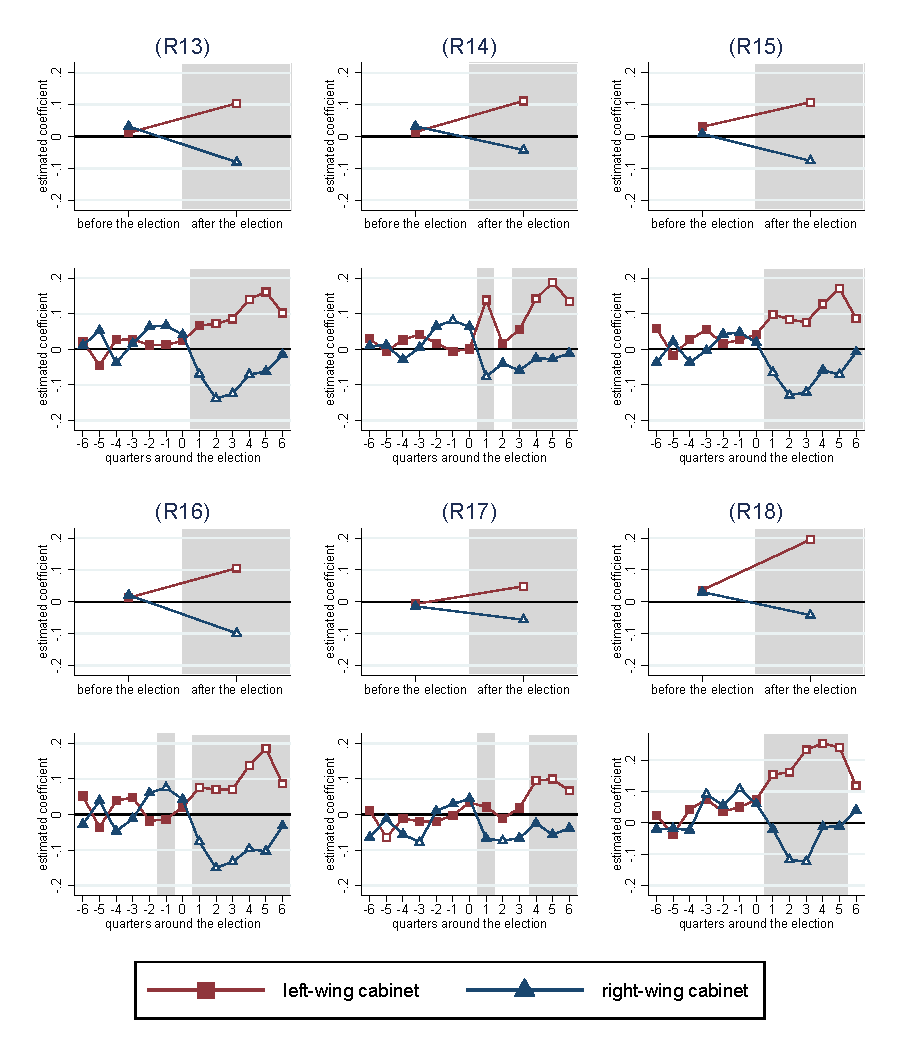
\includegraphics[width=1\textwidth]{../results/applications/app_graphs_R13-R18.pdf}
	\scriptsize{Note: These figures show the time evolution of refugee inflows as estimated in fixed effects regression
		with a set of dummies for before and after the election or a set of dummies for different quarters before and after an election in a quarter t = 0. Significant coefficients are indicated by filled plot markers.}
\end{figure}

\clearpage
\FloatBarrier

\begin{table}[!ht]\centering \footnotesize
\def\sym#1{\ifmmode^{#1}\else\(^{#1}\)\fi}
\caption{Coefficients before after model - R13 - R14}
\begin{tabular}{l*{6}{c}}
\hline\hline
                    &\multicolumn{1}{c}{(1)}&\multicolumn{1}{c}{(2)}&\multicolumn{1}{c}{(3)}&\multicolumn{1}{c}{(4)}&\multicolumn{1}{c}{(5)}&\multicolumn{1}{c}{(6)}\\
                    &\multicolumn{1}{c}{left1\_R13}&\multicolumn{1}{c}{right1\_R13}&\multicolumn{1}{c}{diff1\_R13}&\multicolumn{1}{c}{left1\_R14}&\multicolumn{1}{c}{right1\_R14}&\multicolumn{1}{c}{diff1\_R14}\\
\hline
before              &      0.0127         &      0.0302         &     -0.0175         &      0.0139         &      0.0323         &     -0.0183         \\
                    &    (0.0249)         &    (0.0232)         &    (0.0342)         &    (0.0273)         &    (0.0188)         &    (0.0315)         \\
[1em]
after               &       0.102\sym{***}&     -0.0834\sym{***}&       0.186\sym{***}&       0.110\sym{***}&     -0.0454\sym{*}  &       0.156\sym{***}\\
                    &    (0.0215)         &    (0.0207)         &    (0.0291)         &    (0.0232)         &    (0.0208)         &    (0.0312)         \\
\hline
Observations        &       23705         &       23705         &       23705         &       23705         &       23705         &       23705         \\
\hline\hline
\multicolumn{7}{l}{\footnotesize Standard errors in parentheses}\\
\multicolumn{7}{l}{\footnotesize \sym{*} \(p<0.05\), \sym{**} \(p<0.01\), \sym{***} \(p<0.001\)}\\
\end{tabular}
\end{table}

\begin{table}[!ht]\centering \footnotesize
\def\sym#1{\ifmmode^{#1}\else\(^{#1}\)\fi}
\caption{Coefficients quarterly model - R13 - R14}
\begin{tabular}{l*{6}{c}}
\hline\hline
                    &\multicolumn{1}{c}{(1)}&\multicolumn{1}{c}{(2)}&\multicolumn{1}{c}{(3)}&\multicolumn{1}{c}{(4)}&\multicolumn{1}{c}{(5)}&\multicolumn{1}{c}{(6)}\\
                    &\multicolumn{1}{c}{left2\_R13}&\multicolumn{1}{c}{right2\_R13}&\multicolumn{1}{c}{diff2\_R13}&\multicolumn{1}{c}{left2\_R14}&\multicolumn{1}{c}{right2\_R14}&\multicolumn{1}{c}{diff2\_R14}\\
\hline
 6 quarters before the election&      0.0192         &     0.00723         &      0.0120         &      0.0265         &     0.00628         &      0.0202         \\
                    &    (0.0352)         &    (0.0391)         &    (0.0624)         &    (0.0374)         &    (0.0305)         &    (0.0544)         \\
[1em]
 5 quarters before the election&     -0.0466         &      0.0484         &     -0.0950         &     -0.0115         &      0.0108         &     -0.0222         \\
                    &    (0.0340)         &    (0.0326)         &    (0.0546)         &    (0.0361)         &    (0.0286)         &    (0.0516)         \\
[1em]
 4 quarters before the election&      0.0380         &     -0.0335         &      0.0715         &      0.0361         &     -0.0234         &      0.0595         \\
                    &    (0.0337)         &    (0.0360)         &    (0.0499)         &    (0.0348)         &    (0.0341)         &    (0.0486)         \\
[1em]
 3 quarters before the election&      0.0203         &      0.0162         &     0.00403         &      0.0350         &     0.00449         &      0.0305         \\
                    &    (0.0394)         &    (0.0313)         &    (0.0505)         &    (0.0448)         &    (0.0283)         &    (0.0529)         \\
[1em]
 2 quarters before the election&     0.00859         &      0.0572         &     -0.0486         &      0.0127         &      0.0592         &     -0.0465         \\
                    &    (0.0333)         &    (0.0377)         &    (0.0445)         &    (0.0353)         &    (0.0369)         &    (0.0463)         \\
[1em]
 1 quarters before the election&      0.0115         &      0.0605         &     -0.0490         &    -0.00967         &      0.0784\sym{*}  &     -0.0880\sym{*}  \\
                    &    (0.0362)         &    (0.0350)         &    (0.0419)         &    (0.0379)         &    (0.0353)         &    (0.0447)         \\
[1em]
Quarter of the election&      0.0322         &      0.0420         &    -0.00976         &     0.00870         &      0.0660         &     -0.0573         \\
                    &    (0.0357)         &    (0.0384)         &    (0.0496)         &    (0.0414)         &    (0.0364)         &    (0.0545)         \\
[1em]
 1 quarters after the election&      0.0617         &     -0.0780\sym{**} &       0.140\sym{***}&       0.138\sym{***}&     -0.0869\sym{**} &       0.225\sym{***}\\
                    &    (0.0370)         &    (0.0302)         &    (0.0392)         &    (0.0393)         &    (0.0321)         &    (0.0439)         \\
[1em]
 2 quarters after the election&      0.0702\sym{*}  &      -0.143\sym{***}&       0.213\sym{***}&      0.0142         &     -0.0435         &      0.0576         \\
                    &    (0.0307)         &    (0.0351)         &    (0.0427)         &    (0.0329)         &    (0.0303)         &    (0.0390)         \\
[1em]
 3 quarters after the election&      0.0851\sym{*}  &      -0.129\sym{***}&       0.214\sym{***}&      0.0526         &     -0.0601         &       0.113\sym{*}  \\
                    &    (0.0333)         &    (0.0355)         &    (0.0499)         &    (0.0369)         &    (0.0342)         &    (0.0529)         \\
[1em]
 4 quarters after the election&       0.142\sym{***}&     -0.0659\sym{*}  &       0.208\sym{***}&       0.143\sym{***}&     -0.0206         &       0.163\sym{**} \\
                    &    (0.0293)         &    (0.0327)         &    (0.0456)         &    (0.0365)         &    (0.0314)         &    (0.0532)         \\
[1em]
 5 quarters after the election&       0.154\sym{***}&     -0.0661\sym{*}  &       0.220\sym{***}&       0.183\sym{***}&     -0.0332         &       0.216\sym{***}\\
                    &    (0.0269)         &    (0.0321)         &    (0.0409)         &    (0.0332)         &    (0.0313)         &    (0.0489)         \\
[1em]
 6 quarters after the election&       0.101\sym{**} &     -0.0189         &       0.120\sym{*}  &       0.135\sym{***}&     -0.0149         &       0.149\sym{**} \\
                    &    (0.0309)         &    (0.0309)         &    (0.0489)         &    (0.0305)         &    (0.0291)         &    (0.0462)         \\
\hline
Observations        &       23705         &       23705         &       23705         &       23705         &       23705         &       23705         \\
\hline\hline
\multicolumn{7}{l}{\footnotesize Standard errors in parentheses}\\
\multicolumn{7}{l}{\footnotesize \sym{*} \(p<0.05\), \sym{**} \(p<0.01\), \sym{***} \(p<0.001\)}\\
\end{tabular}
\end{table}

\clearpage
\FloatBarrier
\begin{table}[!ht]\centering \footnotesize
\def\sym#1{\ifmmode^{#1}\else\(^{#1}\)\fi}
\caption{Coefficients before after model - R15 - R16}
\begin{tabular}{l*{6}{c}}
\hline\hline
                    &\multicolumn{3}{c}{(R15)}&\multicolumn{3}{c}{(R16)}\\
&\multicolumn{1}{c}{left}&\multicolumn{1}{c}{right}&\multicolumn{1}{c}{diff}&\multicolumn{1}{c}{left}&\multicolumn{1}{c}{right}&\multicolumn{1}{c}{diff}\\
\hline
before              &      0.0305         &     0.00798         &      0.0226         &      0.0128         &      0.0209         &    -0.00815         \\
                    &    (0.0229)         &    (0.0213)         &    (0.0298)         &    (0.0250)         &    (0.0257)         &    (0.0369)         \\
[0.5em]
after               &       0.108\sym{***}&     -0.0763\sym{***}&       0.184\sym{***}&       0.105\sym{***}&     -0.0992\sym{***}&       0.205\sym{***}\\
                    &    (0.0203)         &    (0.0226)         &    (0.0306)         &    (0.0206)         &    (0.0238)         &    (0.0323)         \\
\hline
Observations        &       25466         &       25466         &       25466         &       22446         &       22446         &       22446         \\
\hline\hline
\multicolumn{7}{l}{ Standard errors in parentheses \sym{*} \(p<0.05\), \sym{**} \(p<0.01\), \sym{***} \(p<0.001\)}\\
\end{tabular}
\end{table}

\begin{table}[!ht]\centering \footnotesize
\def\sym#1{\ifmmode^{#1}\else\(^{#1}\)\fi}
\caption{Coefficients quarterly model - R15 - R16}
\begin{tabular}{l*{6}{c}}
\hline\hline
                    &\multicolumn{3}{c}{(R15)}&\multicolumn{3}{c}{(R16)}\\
&\multicolumn{1}{c}{left}&\multicolumn{1}{c}{right}&\multicolumn{1}{c}{diff}&\multicolumn{1}{c}{left}&\multicolumn{1}{c}{right}&\multicolumn{1}{c}{diff}\\
\hline
 6 quarters before the election&      0.0587         &     -0.0376         &      0.0962         &      0.0517         &     -0.0270         &      0.0788         \\
                    &    (0.0310)         &    (0.0380)         &    (0.0582)         &    (0.0359)         &    (0.0427)         &    (0.0662)         \\
[0.5em]
 5 quarters before the election&     -0.0175         &      0.0212         &     -0.0388         &     -0.0360         &      0.0387         &     -0.0747         \\
                    &    (0.0297)         &    (0.0315)         &    (0.0489)         &    (0.0322)         &    (0.0335)         &    (0.0509)         \\
[0.5em]
 4 quarters before the election&      0.0274         &     -0.0364         &      0.0639         &      0.0385         &     -0.0468         &      0.0853         \\
                    &    (0.0311)         &    (0.0340)         &    (0.0456)         &    (0.0345)         &    (0.0393)         &    (0.0526)         \\
[0.5em]
 3 quarters before the election&      0.0548         &    -0.00400         &      0.0588         &      0.0483         &     -0.0119         &      0.0602         \\
                    &    (0.0396)         &    (0.0294)         &    (0.0473)         &    (0.0446)         &    (0.0306)         &    (0.0551)         \\
[0.5em]
 2 quarters before the election&      0.0157         &      0.0424         &     -0.0267         &     -0.0181         &      0.0605         &     -0.0787         \\
                    &    (0.0316)         &    (0.0382)         &    (0.0430)         &    (0.0329)         &    (0.0387)         &    (0.0463)         \\
[0.5em]
 1 quarters before the election&      0.0267         &      0.0473         &     -0.0206         &     -0.0131         &      0.0755\sym{*}  &     -0.0887\sym{*}  \\
                    &    (0.0351)         &    (0.0311)         &    (0.0391)         &    (0.0356)         &    (0.0370)         &    (0.0441)         \\
[0.5em]
Quarter of the election&      0.0418         &      0.0187         &      0.0231         &      0.0210         &      0.0424         &     -0.0214         \\
                    &    (0.0331)         &    (0.0360)         &    (0.0469)         &    (0.0357)         &    (0.0461)         &    (0.0579)         \\
[0.5em]
 1 quarters after the election&      0.0980\sym{**} &     -0.0655\sym{*}  &       0.164\sym{***}&      0.0758\sym{*}  &     -0.0767\sym{*}  &       0.153\sym{***}\\
                    &    (0.0357)         &    (0.0331)         &    (0.0437)         &    (0.0382)         &    (0.0350)         &    (0.0457)         \\
[0.5em]
 2 quarters after the election&      0.0841\sym{**} &      -0.129\sym{***}&       0.213\sym{***}&      0.0708\sym{*}  &      -0.150\sym{***}&       0.221\sym{***}\\
                    &    (0.0297)         &    (0.0325)         &    (0.0426)         &    (0.0305)         &    (0.0345)         &    (0.0440)         \\
[0.5em]
 3 quarters after the election&      0.0754\sym{*}  &      -0.121\sym{**} &       0.196\sym{***}&      0.0708\sym{*}  &      -0.133\sym{**} &       0.204\sym{***}\\
                    &    (0.0301)         &    (0.0370)         &    (0.0510)         &    (0.0315)         &    (0.0426)         &    (0.0563)         \\
[0.5em]
 4 quarters after the election&       0.127\sym{***}&     -0.0587         &       0.186\sym{***}&       0.138\sym{***}&     -0.0970\sym{**} &       0.235\sym{***}\\
                    &    (0.0283)         &    (0.0353)         &    (0.0460)         &    (0.0278)         &    (0.0337)         &    (0.0439)         \\
[0.5em]
 5 quarters after the election&       0.170\sym{***}&     -0.0711\sym{*}  &       0.241\sym{***}&       0.186\sym{***}&      -0.103\sym{**} &       0.289\sym{***}\\
                    &    (0.0283)         &    (0.0332)         &    (0.0466)         &    (0.0269)         &    (0.0375)         &    (0.0483)         \\
[0.5em]
 6 quarters after the election&      0.0867\sym{**} &    -0.00777         &      0.0944\sym{*}  &      0.0862\sym{**} &     -0.0322         &       0.118\sym{**} \\
                    &    (0.0284)         &    (0.0332)         &    (0.0462)         &    (0.0293)         &    (0.0322)         &    (0.0451)         \\
\hline
Observations        &       25466         &       25466         &       25466         &       22446         &       22446         &       22446         \\
\hline\hline
\multicolumn{7}{l}{ Standard errors in parentheses \sym{*} \(p<0.05\), \sym{**} \(p<0.01\), \sym{***} \(p<0.001\)}\\
\end{tabular}
\end{table}

\clearpage
\FloatBarrier
\begin{table}[!ht]\centering \footnotesize
\def\sym#1{\ifmmode^{#1}\else\(^{#1}\)\fi}
\caption{Coefficients before after model R17 - R18}
\begin{tabular}{l*{6}{c}}
\hline\hline
                    &\multicolumn{1}{c}{(1)}&\multicolumn{1}{c}{(2)}&\multicolumn{1}{c}{(3)}&\multicolumn{1}{c}{(4)}&\multicolumn{1}{c}{(5)}&\multicolumn{1}{c}{(6)}\\
                    &\multicolumn{1}{c}{left1\_R17}&\multicolumn{1}{c}{right1\_R17}&\multicolumn{1}{c}{diff1\_R17}&\multicolumn{1}{c}{left1\_R18}&\multicolumn{1}{c}{right1\_R18}&\multicolumn{1}{c}{diff1\_R18}\\
\hline
before              &    -0.00670         &     -0.0146         &     0.00793         &      0.0381         &      0.0269         &      0.0112         \\
                    &    (0.0237)         &    (0.0252)         &    (0.0355)         &    (0.0325)         &    (0.0305)         &    (0.0479)         \\
[1em]
after               &      0.0487\sym{**} &     -0.0578\sym{*}  &       0.106\sym{***}&       0.193\sym{***}&     -0.0459         &       0.239\sym{***}\\
                    &    (0.0185)         &    (0.0243)         &    (0.0302)         &    (0.0315)         &    (0.0321)         &    (0.0523)         \\
\hline
Observations        &       22391         &       22391         &       22391         &       16488         &       16488         &       16488         \\
\hline\hline
\multicolumn{7}{l}{\footnotesize Standard errors in parentheses}\\
\multicolumn{7}{l}{\footnotesize \sym{*} \(p<0.05\), \sym{**} \(p<0.01\), \sym{***} \(p<0.001\)}\\
\end{tabular}
\end{table}

\begin{table}[htbp]\centering
\def\sym#1{\ifmmode^{#1}\else\(^{#1}\)\fi}
\caption{Coefficients R17 - R18}
\begin{tabular}{l*{4}{c}}
\hline\hline
                    &\multicolumn{1}{c}{(1)}&\multicolumn{1}{c}{(2)}&\multicolumn{1}{c}{(3)}&\multicolumn{1}{c}{(4)}\\
                    &\multicolumn{1}{c}{left\_R17}&\multicolumn{1}{c}{right\_R17}&\multicolumn{1}{c}{left\_R18}&\multicolumn{1}{c}{right\_R18}\\
\hline
 6 quarters before the election&      0.0660\sym{*}  &     -0.0319         &      0.0540         &     -0.0211         \\
                    &    (0.0269)         &    (0.0366)         &    (0.0276)         &    (0.0364)         \\
[1em]
 5 quarters before the election&     -0.0192         &      0.0325         &     -0.0351         &      0.0422         \\
                    &    (0.0296)         &    (0.0311)         &    (0.0294)         &    (0.0311)         \\
[1em]
 4 quarters before the election&      0.0454         &     -0.0318         &      0.0275         &     -0.0359         \\
                    &    (0.0368)         &    (0.0380)         &    (0.0360)         &    (0.0381)         \\
[1em]
 3 quarters before the election&      0.0474         &      0.0169         &      0.0327         &      0.0127         \\
                    &    (0.0436)         &    (0.0296)         &    (0.0434)         &    (0.0298)         \\
[1em]
 2 quarters before the election&      0.0209         &      0.0544         &     0.00536         &      0.0641         \\
                    &    (0.0359)         &    (0.0380)         &    (0.0355)         &    (0.0390)         \\
[1em]
 1 quarters before the election&      0.0114         &      0.0538         &     0.00449         &      0.0569         \\
                    &    (0.0423)         &    (0.0369)         &    (0.0425)         &    (0.0368)         \\
[1em]
Quarter of the election&      0.0340         &      0.0191         &      0.0330         &      0.0317         \\
                    &    (0.0392)         &    (0.0379)         &    (0.0393)         &    (0.0374)         \\
[1em]
 1 quarters after the election&      0.0611         &     -0.0764\sym{*}  &      0.0757\sym{*}  &     -0.0742\sym{*}  \\
                    &    (0.0372)         &    (0.0367)         &    (0.0373)         &    (0.0366)         \\
[1em]
 2 quarters after the election&      0.0743\sym{*}  &      -0.142\sym{***}&      0.0742\sym{*}  &      -0.118\sym{***}\\
                    &    (0.0345)         &    (0.0340)         &    (0.0347)         &    (0.0343)         \\
[1em]
 3 quarters after the election&      0.0825\sym{*}  &      -0.135\sym{**} &      0.0822\sym{*}  &      -0.121\sym{**} \\
                    &    (0.0337)         &    (0.0454)         &    (0.0339)         &    (0.0443)         \\
[1em]
 4 quarters after the election&       0.137\sym{***}&     -0.0808\sym{*}  &       0.135\sym{***}&     -0.0692         \\
                    &    (0.0315)         &    (0.0385)         &    (0.0315)         &    (0.0386)         \\
[1em]
 5 quarters after the election&       0.180\sym{***}&     -0.0953\sym{**} &       0.181\sym{***}&     -0.0860\sym{*}  \\
                    &    (0.0282)         &    (0.0352)         &    (0.0282)         &    (0.0353)         \\
[1em]
 6 quarters after the election&      0.0927\sym{***}&     -0.0141         &      0.0951\sym{***}&    -0.00180         \\
                    &    (0.0263)         &    (0.0300)         &    (0.0260)         &    (0.0294)         \\
\hline
Observations        &       23705         &       23705         &       23705         &       23705         \\
\hline\hline
\multicolumn{5}{l}{\footnotesize Standard errors in parentheses}\\
\multicolumn{5}{l}{\footnotesize \sym{*} \(p<0.05\), \sym{**} \(p<0.01\), \sym{***} \(p<0.001\)}\\
\end{tabular}
\end{table}



\clearpage
\FloatBarrier
\begin{table}[htbp]\centering  \footnotesize
\def\sym#1{\ifmmode^{#1}\else\(^{#1}\)\fi}
\caption{Determinants of first-time asylum applications per capita - R19 - R22}
\begin{tabular}{l*{4}{c}}
\hline\hline
                    &\multicolumn{1}{c}{(R19)}         &\multicolumn{1}{c}{(R20)}         &\multicolumn{1}{c}{(R21)}         &\multicolumn{1}{c}{(R22)}         \\
\hline
Political Terror Scale&       0.399\sym{***}&       0.399\sym{***}&       0.399\sym{***}&       0.410\sym{***}\\
                    &    (0.0696)         &    (0.0696)         &    (0.0743)         &    (0.0849)         \\
[0,5em]
Civic Liberty (FHI) &       0.175         &       0.175         &       0.155         &       0.172         \\
                    &     (0.131)         &     (0.131)         &     (0.129)         &     (0.143)         \\
[0,5em]
Political Rights (FHI)&      0.0482         &      0.0484         &      0.0453         &      0.0513         \\
                    &    (0.0749)         &    (0.0751)         &    (0.0745)         &    (0.0785)         \\
[0,5em]
Quarterly civil war&       0.188\sym{***}&       0.188\sym{***}&       0.198\sym{***}&       0.186\sym{***}\\
 battle death (000s)                    &    (0.0234)         &    (0.0234)         &    (0.0241)         &    (0.0232)         \\
[0,5em]
Log origin country &      -0.660\sym{***}&      -0.662\sym{***}&      -0.595\sym{***}&      -0.766\sym{***}\\
real GDP per capita                    &     (0.163)         &     (0.163)         &     (0.159)         &     (0.170)         \\
[0,5em]
Log destination country&      -1.494\sym{**} &      -1.472\sym{**} &      -0.264         &      -1.771\sym{***}\\
 real GDP per capita                    &     (0.439)         &     (0.439)         &     (0.439)         &     (0.471)         \\
[0,5em]
Quarterly unemployment&     -0.0750\sym{***}&     -0.0742\sym{***}&     -0.0112         &     -0.0737\sym{***}\\
 rate at destination                    &    (0.0108)         &    (0.0108)         &   (0.00953)         &    (0.0112)         \\
[0,5em]
Log average total first-time applications &                     &                     &   0.703\sym{***}                   &                     \\
 in the previous 6 quarters                    &                     &                     &     (0.0501)                 &                     \\
[0,5em]
Nationalist party in parliament&       0.246\sym{***}&                     &                     &                     \\
                    &    (0.0623)         &                     &                     &                     \\
[0,5em]
Share of nationalist parties &                     &       1.715\sym{**} &                     &                     \\
in parliament                    &                     &     (0.626)         &                     &                     \\
[0,5em]
Cabinet position left *&      0.0369         &      0.0263         &     0.00208         &      0.0364         \\
 Before the election                    &    (0.0242)         &    (0.0243)         &    (0.0233)         &    (0.0324)         \\
[0,5em]
Cabinet position left * &       0.113\sym{***}&       0.116\sym{***}&      0.0576\sym{**} &       0.195\sym{***}\\
After the election                    &    (0.0213)         &    (0.0213)         &    (0.0196)         &    (0.0316)         \\
[0,5em]
Cabinet position right * &     0.00935         &      0.0141         &     -0.0204         &      0.0306         \\
Before the election                    &    (0.0235)         &    (0.0235)         &    (0.0236)         &    (0.0305)         \\
[0,5em]
Cabinet position right *&     -0.0985\sym{***}&     -0.0877\sym{***}&     -0.0572\sym{*}  &     -0.0419         \\
 After the election                    &    (0.0228)         &    (0.0226)         &    (0.0228)         &    (0.0319)         \\
\hline
Observations        &       23705         &       23705         &       23642         &       16488         \\
Adjusted \(R^{2}\)  &       0.179         &       0.177         &       0.239         &       0.183         \\
Fixed Effects       &       D x O         &       D x O         &       D x O         &       D x O         \\
Destination dummies &          No         &          No         &          No         &          No         \\
Quarter-Year dummies&         Yes         &         Yes         &         Yes         &         Yes         \\
\hline\hline
\multicolumn{5}{l}{Standard errors in parentheses \sym{*} \(p<0.05\), \sym{**} \(p<0.01\), \sym{***} \(p<0.001\)}\\
\end{tabular}
\end{table}


\clearpage
\FloatBarrier
\begin{figure}[!ht]
	\caption{First-time asylum applications per capita: predicted pattern - R19 to R22}
	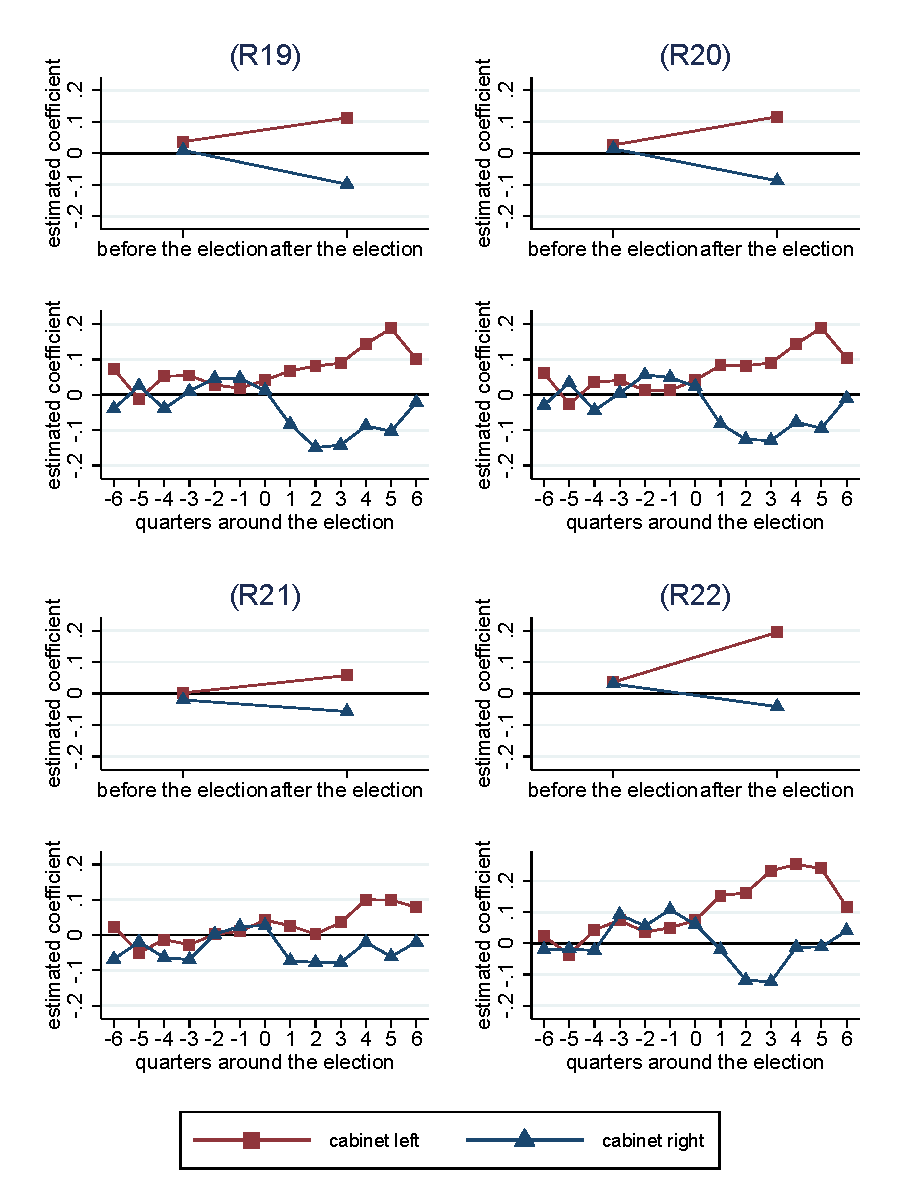
\includegraphics[width=1\textwidth]{../results/applications/app_graphs_R19-R22.pdf}
	\scriptsize{Note: These figures show the time evolution of refugee inflows as estimated in fixed effects regression
		with a set of dummies for before and after the election or a set of dummies for different quarters before and after an election in a quarter t = 0. Significant coefficients are indicated by filled plot markers.}
\end{figure}

\clearpage
\FloatBarrier

\begin{table}[!ht]\centering \footnotesize
\def\sym#1{\ifmmode^{#1}\else\(^{#1}\)\fi}
\caption{Coefficients before after model - R19 - R20}
\begin{tabular}{l*{6}{c}}
\hline\hline
                    &\multicolumn{3}{c}{(R19)}&\multicolumn{3}{c}{(R20)}\\
&\multicolumn{1}{c}{left}&\multicolumn{1}{c}{right}&\multicolumn{1}{c}{diff}&\multicolumn{1}{c}{left}&\multicolumn{1}{c}{right}&\multicolumn{1}{c}{diff}\\
\hline
before              &      0.0369         &     0.00935         &      0.0276         &      0.0263         &      0.0141         &      0.0122         \\
                    &    (0.0242)         &    (0.0235)         &    (0.0341)         &    (0.0243)         &    (0.0235)         &    (0.0339)         \\
[0.5em]
after               &       0.113\sym{***}&     -0.0985\sym{***}&       0.211\sym{***}&       0.116\sym{***}&     -0.0877\sym{***}&       0.204\sym{***}\\
                    &    (0.0213)         &    (0.0228)         &    (0.0314)         &    (0.0213)         &    (0.0226)         &    (0.0313)         \\
\hline
Observations        &       23705         &       23705         &       23705         &       23705         &       23705         &       23705         \\
\hline\hline
\multicolumn{7}{l}{ Standard errors in parentheses \sym{*} \(p<0.05\), \sym{**} \(p<0.01\), \sym{***} \(p<0.001\)}\\
\end{tabular}
\end{table}

\begin{table}[htbp]\centering
\def\sym#1{\ifmmode^{#1}\else\(^{#1}\)\fi}
\caption{Coefficients R19 - R20}
\begin{tabular}{l*{4}{c}}
\hline\hline
                    &\multicolumn{1}{c}{(1)}&\multicolumn{1}{c}{(2)}&\multicolumn{1}{c}{(3)}&\multicolumn{1}{c}{(4)}\\
                    &\multicolumn{1}{c}{left\_R19}&\multicolumn{1}{c}{right\_R19}&\multicolumn{1}{c}{left\_R20}&\multicolumn{1}{c}{right\_R20}\\
\hline
 6 quarters before the election&      0.0555         &     -0.0244         &     0.00924         &    -0.00805         \\
                    &    (0.0358)         &    (0.0352)         &    (0.0354)         &    (0.0398)         \\
[1em]
 5 quarters before the election&     -0.0294         &      0.0385         &     -0.0507         &    -0.00629         \\
                    &    (0.0349)         &    (0.0344)         &    (0.0421)         &    (0.0350)         \\
[1em]
 4 quarters before the election&      0.0333         &     -0.0422         &      0.0295         &     -0.0115         \\
                    &    (0.0447)         &    (0.0375)         &    (0.0526)         &    (0.0422)         \\
[1em]
 3 quarters before the election&      0.0398         &     0.00650         &      0.0614         &       0.103\sym{**} \\
                    &    (0.0489)         &    (0.0429)         &    (0.0533)         &    (0.0370)         \\
[1em]
 2 quarters before the election&     0.00828         &      0.0600         &      0.0224         &      0.0669         \\
                    &    (0.0449)         &    (0.0433)         &    (0.0477)         &    (0.0476)         \\
[1em]
 1 quarters before the election&     0.00414         &      0.0701         &      0.0358         &       0.119\sym{*}  \\
                    &    (0.0445)         &    (0.0427)         &    (0.0579)         &    (0.0515)         \\
[1em]
Quarter of the election&      0.0325         &      0.0293         &      0.0590         &      0.0710         \\
                    &    (0.0430)         &    (0.0414)         &    (0.0538)         &    (0.0460)         \\
[1em]
 1 quarters after the election&      0.0775         &     -0.0698         &       0.139\sym{***}&    -0.00895         \\
                    &    (0.0421)         &    (0.0400)         &    (0.0423)         &    (0.0393)         \\
[1em]
 2 quarters after the election&      0.0697         &      -0.136\sym{***}&       0.148\sym{**} &      -0.106\sym{*}  \\
                    &    (0.0412)         &    (0.0412)         &    (0.0459)         &    (0.0427)         \\
[1em]
 3 quarters after the election&      0.0774\sym{*}  &      -0.127\sym{**} &       0.219\sym{***}&      -0.112\sym{*}  \\
                    &    (0.0389)         &    (0.0412)         &    (0.0463)         &    (0.0443)         \\
[1em]
 4 quarters after the election&       0.131\sym{***}&     -0.0733         &       0.239\sym{***}&   -0.000831         \\
                    &    (0.0376)         &    (0.0425)         &    (0.0390)         &    (0.0401)         \\
[1em]
 5 quarters after the election&       0.173\sym{***}&     -0.0904\sym{*}  &       0.226\sym{***}&    0.000330         \\
                    &    (0.0359)         &    (0.0400)         &    (0.0379)         &    (0.0401)         \\
[1em]
 6 quarters after the election&      0.0899\sym{**} &    -0.00688         &       0.103\sym{**} &      0.0512         \\
                    &    (0.0324)         &    (0.0324)         &    (0.0314)         &    (0.0313)         \\
\hline
Observations        &       23705         &       23705         &       16488         &       16488         \\
\hline\hline
\multicolumn{5}{l}{\footnotesize Standard errors in parentheses}\\
\multicolumn{5}{l}{\footnotesize \sym{*} \(p<0.05\), \sym{**} \(p<0.01\), \sym{***} \(p<0.001\)}\\
\end{tabular}
\end{table}

\clearpage
\FloatBarrier
\begin{table}[!ht]\centering \footnotesize
\def\sym#1{\ifmmode^{#1}\else\(^{#1}\)\fi}
\caption{Coefficients before after model - R21 - R22}
\begin{tabular}{l*{6}{c}}
\hline\hline
                    &\multicolumn{3}{c}{(R21)}&\multicolumn{3}{c}{(R22)}\\
&\multicolumn{1}{c}{left}&\multicolumn{1}{c}{right}&\multicolumn{1}{c}{diff}&\multicolumn{1}{c}{left}&\multicolumn{1}{c}{right}&\multicolumn{1}{c}{diff}\\
\hline
before              &     0.00208         &     -0.0204         &      0.0225         &      0.0364         &      0.0306         &     0.00584         \\
                    &    (0.0233)         &    (0.0236)         &    (0.0336)         &    (0.0324)         &    (0.0305)         &    (0.0480)         \\
[0.5em]
after               &      0.0576\sym{**} &     -0.0572\sym{*}  &       0.115\sym{***}&       0.195\sym{***}&     -0.0419         &       0.237\sym{***}\\
                    &    (0.0196)         &    (0.0228)         &    (0.0291)         &    (0.0316)         &    (0.0319)         &    (0.0522)         \\
\hline
Observations        &       23642         &       23642         &       23642         &       16488         &       16488         &       16488         \\
\hline\hline
\multicolumn{7}{l}{ Standard errors in parentheses \sym{*} \(p<0.05\), \sym{**} \(p<0.01\), \sym{***} \(p<0.001\)}\\
\end{tabular}
\end{table}

\begin{table}[!ht]\centering \footnotesize
\def\sym#1{\ifmmode^{#1}\else\(^{#1}\)\fi}
\caption{Coefficients quarterly model - R21 - R22}
\begin{tabular}{l*{6}{c}}
\hline\hline
                    &\multicolumn{3}{c}{(R21)}&\multicolumn{3}{c}{(R22)}\\
&\multicolumn{1}{c}{left}&\multicolumn{1}{c}{right}&\multicolumn{1}{c}{diff}&\multicolumn{1}{c}{left}&\multicolumn{1}{c}{right}&\multicolumn{1}{c}{diff}\\
\hline
 6 quarters before the election&      0.0235         &     -0.0679         &      0.0914         &      0.0231         &     -0.0198         &      0.0429         \\
                    &    (0.0337)         &    (0.0427)         &    (0.0644)         &    (0.0475)         &    (0.0480)         &    (0.0799)         \\
[0.5em]
 5 quarters before the election&     -0.0496         &     -0.0197         &     -0.0298         &     -0.0368         &     -0.0180         &     -0.0187         \\
                    &    (0.0311)         &    (0.0346)         &    (0.0544)         &    (0.0480)         &    (0.0362)         &    (0.0709)         \\
[0.5em]
 4 quarters before the election&     -0.0132         &     -0.0636         &      0.0504         &      0.0429         &     -0.0230         &      0.0658         \\
                    &    (0.0330)         &    (0.0368)         &    (0.0508)         &    (0.0499)         &    (0.0402)         &    (0.0698)         \\
[0.5em]
 3 quarters before the election&     -0.0272         &     -0.0695\sym{*}  &      0.0423         &      0.0747         &      0.0917\sym{*}  &     -0.0170         \\
                    &    (0.0393)         &    (0.0300)         &    (0.0511)         &    (0.0480)         &    (0.0360)         &    (0.0631)         \\
[0.5em]
 2 quarters before the election&     0.00197         &     0.00282         &   -0.000855         &      0.0358         &      0.0557         &     -0.0199         \\
                    &    (0.0327)         &    (0.0369)         &    (0.0452)         &    (0.0410)         &    (0.0458)         &    (0.0587)         \\
[0.5em]
 1 quarters before the election&      0.0110         &      0.0241         &     -0.0131         &      0.0502         &       0.108\sym{*}  &     -0.0579         \\
                    &    (0.0358)         &    (0.0347)         &    (0.0421)         &    (0.0467)         &    (0.0505)         &    (0.0680)         \\
[0.5em]
Quarter of the election&      0.0424         &      0.0269         &      0.0155         &      0.0738         &      0.0603         &      0.0135         \\
                    &    (0.0336)         &    (0.0373)         &    (0.0451)         &    (0.0455)         &    (0.0529)         &    (0.0695)         \\
[0.5em]
 1 quarters after the election&      0.0265         &     -0.0728\sym{*}  &      0.0993\sym{*}  &       0.153\sym{***}&     -0.0203         &       0.174\sym{**} \\
                    &    (0.0374)         &    (0.0323)         &    (0.0438)         &    (0.0413)         &    (0.0381)         &    (0.0591)         \\
[0.5em]
 2 quarters after the election&     0.00249         &     -0.0773\sym{*}  &      0.0798\sym{*}  &       0.162\sym{***}&      -0.118\sym{*}  &       0.279\sym{***}\\
                    &    (0.0270)         &    (0.0342)         &    (0.0369)         &    (0.0409)         &    (0.0469)         &    (0.0653)         \\
[0.5em]
 3 quarters after the election&      0.0357         &     -0.0777         &       0.113\sym{*}  &       0.233\sym{***}&      -0.123\sym{**} &       0.356\sym{***}\\
                    &    (0.0320)         &    (0.0401)         &    (0.0526)         &    (0.0450)         &    (0.0439)         &    (0.0720)         \\
[0.5em]
 4 quarters after the election&      0.1000\sym{***}&     -0.0206         &       0.121\sym{**} &       0.253\sym{***}&     -0.0124         &       0.266\sym{***}\\
                    &    (0.0264)         &    (0.0334)         &    (0.0426)         &    (0.0356)         &    (0.0430)         &    (0.0621)         \\
[0.5em]
 5 quarters after the election&      0.0990\sym{***}&     -0.0609         &       0.160\sym{***}&       0.240\sym{***}&     -0.0116         &       0.252\sym{***}\\
                    &    (0.0260)         &    (0.0352)         &    (0.0442)         &    (0.0401)         &    (0.0502)         &    (0.0719)         \\
[0.5em]
 6 quarters after the election&      0.0791\sym{**} &     -0.0198         &      0.0988\sym{*}  &       0.118\sym{**} &      0.0401         &      0.0779         \\
                    &    (0.0296)         &    (0.0335)         &    (0.0498)         &    (0.0438)         &    (0.0400)         &    (0.0734)         \\
\hline
Observations        &       23642         &       23642         &       23642         &       16488         &       16488         &       16488         \\
\hline\hline
\multicolumn{7}{l}{ Standard errors in parentheses \sym{*} \(p<0.05\), \sym{**} \(p<0.01\), \sym{***} \(p<0.001\)}\\
\end{tabular}
\end{table}



\clearpage
\FloatBarrier
\section{Robustness Checks for Decision Analysis}
Robustness check 1 to 6 and 10 are analogous to the robustness checks in the application analysis.

\begin{itemize}
	\item \textbf{Robustness Check 1}: In this robustness check we use separate fixed effects for destination and origin instead of a fixed effect for each destination-origin pair. This specification allows to include time-invariant bilateral variables in the regression, such as the distance between destination and origin country and the stock of migrants from a certain origin country in the destination country in 2001. In the regression both variables are included in logs. All other control variables are the same as in the baseline regression.  
	
	\item \textbf{Robustness Check 2}: In this robustness check we use destination fixed effects as well as origin*time fixed effects. All time-variant origin country control variables are captured by the origin*time fixed effects and therefore not included in this specification. Similar to robustness check 1, this specification also allows to include time-invariant bilateral variables.  
	
	\item \textbf{Robustness Check 3}: In this robustness check the log of the average total past asylum applications at destination per capita in the previous 5 years is included as an additional destination control variable. 
	
	\item \textbf{Robustness Check 4}: In order to allow for different effects of left-wing and right-wing cabinets outside the election period, this robustness check includes a dummy which is equal to 1 if the incumbent cabinet is classified as right-wing.   
	
	\item \textbf{Robustness Check 5}: In this robustness check we use the overall asylum policy index provided by Hatton (2017), which measures the strictness of asylum policies in destination countries as an additional control variable.
	
	\item \textbf{Robustness Check 6}: In comparison to robustness check 5, in this robustness check we include the separate asylum policy indices for the areas access, welfare and processing. 
	
	\item \textbf{Robustness Check 7}: In this robustness check we control for the log total decisions at the destination per capita instead of the log dyadic decisions per capita in the current quarter.
	
	\item \textbf{Robustness Check 8}: In this robustness check we control for both, the log dyadic decisions per capita and the log total decisions at destination per capita. 
	
	\item \textbf{Robustness Check 9}: In this robustness check the destination country sample includes all large countries in terms of asylum decisions for which decision data is available in at least 44 out of the 52 quarters under analysis. The countries that are added are Austria, Finland, Greece and Hungary.  
	
	\item \textbf{Robustness Check 10}: As there have been some changes in the data collection method of the asylum data by Eurostat in 2008, in this robustness check we include a dummy which is equal to 1 if the year is 2008 or later and zero otherwise as an additional control variable. 
	
	\item \textbf{Robustness Check 11 to 16}:  In robustness checks 11 to 16 we no longer include the log dyadic decisions per capita in the current quarter in the regression but instead some alternative measure of total decisions or total first-time applications. For robustness check 11 to 13 we calculate the log of the average total and the average dyadic decisions in the current and the previous 3 quarters per capita. In robustness check 11 we only use the variable with the total decisions at destination, in robustness check 12 we only use the variable with the dyadic decisions and in robustness check 13 we use both the variable with the total and the variable with the dyadic decisions. For robustness checks 14 to 16 we calculate the log of the total and the dyadic number of first time applications per capita in the previous 2 quarters. For robustness check 14 we use only the variable with the total first-time applications, in robustness check 15 we use only the variable with the dyadic first-time applications and finally in robustness check 16 we use both the variable with the total and the variable with the dyadic first-time applications.  
 
	\item \textbf{Robustness Check 17 to 20}: For robustness check 17 to 20 we change the dependent variables. We no longer use log decisions per capita, but instead we calculate the share of total decisions which result in any kind of protection (acceptance rate), in refugee status according to the Geneva Convention (refugee status rate) and in some other form temporary protection (temporary protection rate). As the number of total decisions in the quarter is already used when calculating the dependent variables we do not control for the log total dyadic decisions per capita in the current quarter in any of these robustness checks. In robustness check 17 we add no additional controls. In robustness check 18 we include a dummy which is equal to 1 if the incumbent cabinet's position is right-wing. In robustness check 19 we control for the log of the average total and the log of the average dyadic decision per capita in the current and the previous 3 quarters. And finally in robustness check 20 we control for the log of the average total and the log of the average dyadic first-time applications per capita in the previous 2 quarters.
	 
\end{itemize}	
	

\clearpage
\FloatBarrier
\begin{table}[!ht]\centering \scriptsize
\def\sym#1{\ifmmode^{#1}\else\(^{#1}\)\fi}
\caption{Determinants of asylum decisions}
\begin{tabular}{l*{3}{c}}
\hline\hline
Dependent variable                    &\multicolumn{1}{c}{Acceptance rate}&\multicolumn{1}{c}{Refugee status rate}&\multicolumn{1}{c}{Temporary protection rate}\\
\hline
Political Terror Scale&      0.0269\sym{*}  &      0.0297\sym{**} &    -0.00281         \\
                    &    (0.0109)         &   (0.00860)         &   (0.00629)         \\
[0.5em]
Civic Liberty (FHI) &      0.0345         &      0.0219         &      0.0126         \\
                    &    (0.0226)         &    (0.0145)         &   (0.00993)         \\
[0.5em]
Political Rights (FHI)&    -0.00792         &    -0.00961         &     0.00169         \\
                    &    (0.0199)         &    (0.0116)         &   (0.00924)         \\
[0.5em]
Quarterly civil war &      0.0532\sym{***}&      0.0160\sym{***}&      0.0372\sym{***}\\
battle death (000s)                    &   (0.00503)         &   (0.00323)         &   (0.00263)         \\
[0.5em]
Log origin country &     -0.0227         &     -0.0135         &    -0.00921         \\
real GDP per capita                    &    (0.0322)         &    (0.0252)         &    (0.0111)         \\
[0.5em]
Log destination country&       0.223\sym{*}  &      -0.131\sym{*}  &       0.354\sym{***}\\
 quarterly real GDP per capita                    &    (0.0863)         &    (0.0598)         &    (0.0777)         \\
[0.5em]
Quarterly unemployment &  -0.0000658         &    -0.00402\sym{*}  &     0.00395\sym{*}  \\
rate at destination                    &   (0.00115)         &   (0.00161)         &   (0.00161)         \\
[0.5em]
Cabinet position left * &     0.00568         &     -0.0168\sym{**} &      0.0225\sym{***}\\
 Before the election                   &   (0.00771)         &   (0.00530)         &   (0.00483)         \\
[0.5em]
Cabinet position left * &     -0.0256\sym{**} &     -0.0257\sym{***}&   0.0000830         \\
 After the election                   &   (0.00760)         &   (0.00534)         &   (0.00377)         \\
[0.5em]
Cabinet position right * &     -0.0118         &    -0.00716         &    -0.00469         \\
 Before the election                   &   (0.00738)         &   (0.00564)         &   (0.00519)         \\
[0.5em]
Cabinet position right * &      0.0496\sym{***}&      0.0123\sym{**} &      0.0373\sym{***}\\
After the election                    &   (0.00904)         &   (0.00416)         &   (0.00823)         \\
\hline
Observations        &       12921         &       12921         &       12921         \\
Adjusted \(R^{2}\)  &       0.134         &       0.083         &       0.067         \\
Mean dependent variable&       0.159         &      0.0866         &      0.0725         \\
Fixed Effects       &       D x O         &       D x O         &       D x O         \\
Destination dummies &          No         &          No         &          No         \\
Quarter-Year dummies&         Yes         &         Yes         &         Yes         \\
\hline\hline
\multicolumn{4}{l}{Standard errors in parentheses \sym{*} \(p<0.05\), \sym{**} \(p<0.01\), \sym{***} \(p<0.001\)}\\
\end{tabular}
\label{dec_table1_baseline}
\end{table}


\clearpage
\FloatBarrier
\begin{figure}[!ht]
	
	\caption{Asylum decisions per capita: predicted pattern - baseline}
	\centering
	\begin{minipage}{0.9\textwidth} 
		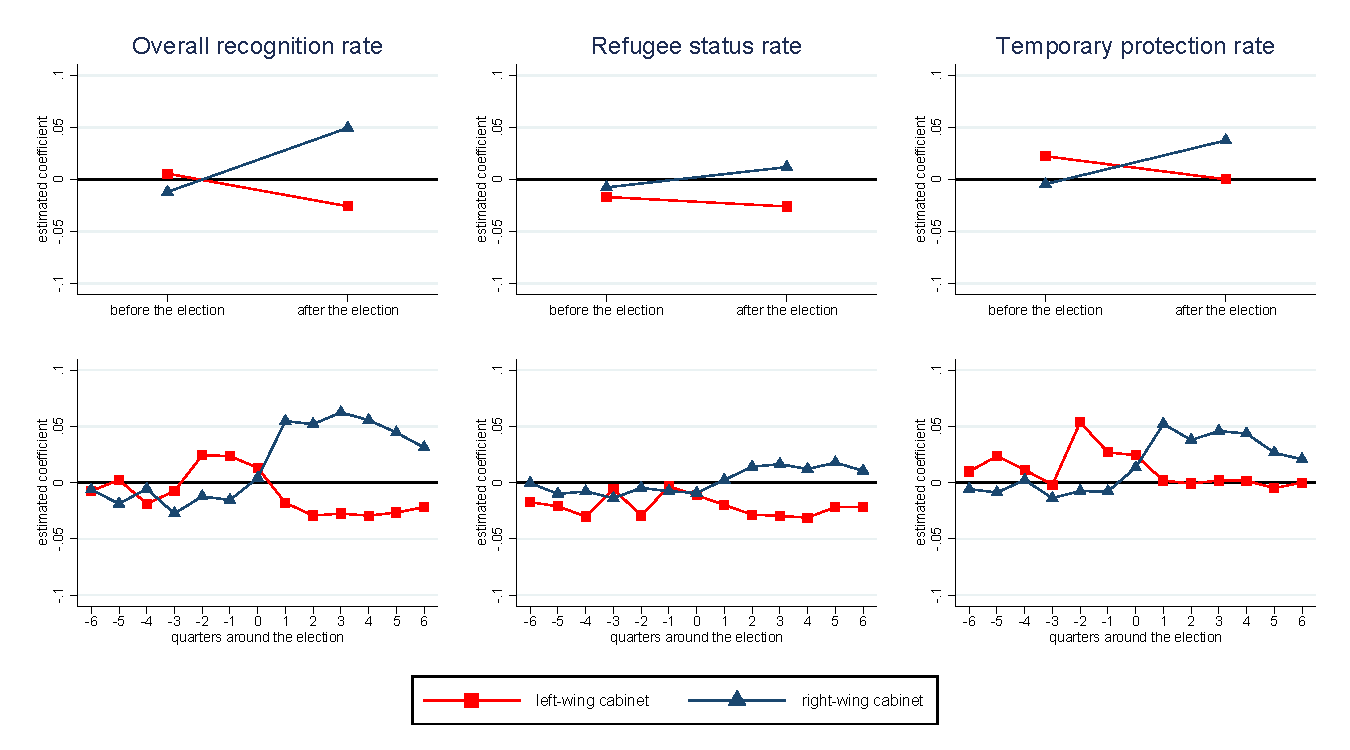
\includegraphics[width=\linewidth]{../results/decisions/dec_graphs_baseline.pdf}
		{\scriptsize Note: These figures show the time evolution of positive decisions, refugee status decisions and temporary protection decisions as estimated in fixed effects regression with a set of dummies for before and after the election or a set of dummies for different quarters before and after an election in a quarter t = 0. Significant coefficients are indicated by filled plot markers. In addition to the controls that are specified in equation (XXX) in all decision regressions we control for the log of the total dyadic decisions per capita unless mentioned otherwise in the robustness checks.\par}
	\end{minipage}
\end{figure}

\begin{table}[htbp]\centering
\def\sym#1{\ifmmode^{#1}\else\(^{#1}\)\fi}
\caption{Coefficients quarterly model Decisions}
\begin{tabular}{l*{6}{c}}
\hline\hline
                    &\multicolumn{1}{c}{(1)}&\multicolumn{1}{c}{(2)}&\multicolumn{1}{c}{(3)}&\multicolumn{1}{c}{(4)}&\multicolumn{1}{c}{(5)}&\multicolumn{1}{c}{(6)}\\
                    &\multicolumn{1}{c}{left\_pos}&\multicolumn{1}{c}{right\_pos}&\multicolumn{1}{c}{left\_ref}&\multicolumn{1}{c}{right\_ref}&\multicolumn{1}{c}{left\_temp}&\multicolumn{1}{c}{right\_temp}\\
\hline
 6 quarters before the election&     0.00309         &     -0.0993\sym{***}&      -0.110\sym{**} &     -0.0108         &      0.0519         &      -0.135\sym{***}\\
                    &    (0.0319)         &    (0.0290)         &    (0.0391)         &    (0.0257)         &    (0.0336)         &    (0.0306)         \\
[1em]
 5 quarters before the election&      0.0681         &     -0.0678         &      -0.115\sym{**} &     -0.0134         &       0.146\sym{***}&     -0.0941\sym{**} \\
                    &    (0.0437)         &    (0.0369)         &    (0.0382)         &    (0.0358)         &    (0.0409)         &    (0.0288)         \\
[1em]
 4 quarters before the election&     -0.0393         &     -0.0384         &      -0.209\sym{***}&     -0.0624         &      0.0917\sym{*}  &    -0.00152         \\
                    &    (0.0533)         &    (0.0374)         &    (0.0439)         &    (0.0398)         &    (0.0432)         &    (0.0349)         \\
[1em]
 3 quarters before the election&      0.0531         &     -0.0583         &      -0.107\sym{**} &     -0.0289         &      0.0961\sym{*}  &     -0.0539         \\
                    &    (0.0428)         &    (0.0443)         &    (0.0369)         &    (0.0479)         &    (0.0403)         &    (0.0348)         \\
[1em]
 2 quarters before the election&       0.177\sym{***}&     -0.0252         &      -0.177\sym{***}&     -0.0218         &       0.269\sym{***}&      0.0147         \\
                    &    (0.0425)         &    (0.0466)         &    (0.0402)         &    (0.0386)         &    (0.0359)         &    (0.0459)         \\
[1em]
 1 quarters before the election&       0.158\sym{**} &      0.0238         &     -0.0584         &      0.0542         &       0.166\sym{***}&      0.0449         \\
                    &    (0.0529)         &    (0.0516)         &    (0.0390)         &    (0.0437)         &    (0.0407)         &    (0.0464)         \\
[1em]
Quarter of the election&      0.0460         &      0.0489         &      -0.106\sym{*}  &      0.0178         &      0.0803\sym{*}  &      0.0618         \\
                    &    (0.0450)         &    (0.0415)         &    (0.0414)         &    (0.0305)         &    (0.0327)         &    (0.0429)         \\
[1em]
 1 quarters after the election&    -0.00651         &       0.142\sym{**} &      -0.100\sym{**} &      0.0765\sym{*}  &      0.0516         &      0.0997\sym{*}  \\
                    &    (0.0428)         &    (0.0478)         &    (0.0387)         &    (0.0320)         &    (0.0338)         &    (0.0465)         \\
[1em]
 2 quarters after the election&     -0.0521         &       0.142\sym{**} &      -0.107\sym{**} &       0.111\sym{**} &      0.0644\sym{*}  &      0.0651         \\
                    &    (0.0374)         &    (0.0452)         &    (0.0394)         &    (0.0343)         &    (0.0316)         &    (0.0455)         \\
[1em]
 3 quarters after the election&     -0.0284         &       0.224\sym{***}&      -0.107\sym{**} &       0.128\sym{***}&      0.0953\sym{**} &       0.137\sym{**} \\
                    &    (0.0339)         &    (0.0330)         &    (0.0354)         &    (0.0295)         &    (0.0295)         &    (0.0432)         \\
[1em]
 4 quarters after the election&     -0.0467         &       0.194\sym{***}&      -0.120\sym{***}&      0.0852\sym{*}  &      0.0993\sym{***}&       0.114\sym{**} \\
                    &    (0.0348)         &    (0.0330)         &    (0.0352)         &    (0.0358)         &    (0.0297)         &    (0.0415)         \\
[1em]
 5 quarters after the election&  -0.0000619         &       0.170\sym{***}&     -0.0910\sym{**} &       0.109\sym{***}&      0.0936\sym{**} &       0.121\sym{**} \\
                    &    (0.0350)         &    (0.0399)         &    (0.0339)         &    (0.0330)         &    (0.0348)         &    (0.0414)         \\
[1em]
 6 quarters after the election&     -0.0324         &       0.100\sym{***}&      -0.131\sym{**} &      0.0943\sym{**} &       0.108\sym{***}&      0.0336         \\
                    &    (0.0418)         &    (0.0293)         &    (0.0441)         &    (0.0290)         &    (0.0310)         &    (0.0342)         \\
\hline
Observations        &       15938         &       15938         &       15938         &       15938         &       15938         &       15938         \\
\hline\hline
\multicolumn{7}{l}{\footnotesize Standard errors in parentheses}\\
\multicolumn{7}{l}{\footnotesize \sym{*} \(p<0.05\), \sym{**} \(p<0.01\), \sym{***} \(p<0.001\)}\\
\end{tabular}
\end{table}



\clearpage
\FloatBarrier
\begin{figure}[!ht]
	
	\caption{Asylum decisions per capita: predicted pattern - include cabinet right dummy}
	\centering
	\begin{minipage}{0.9\textwidth} 
		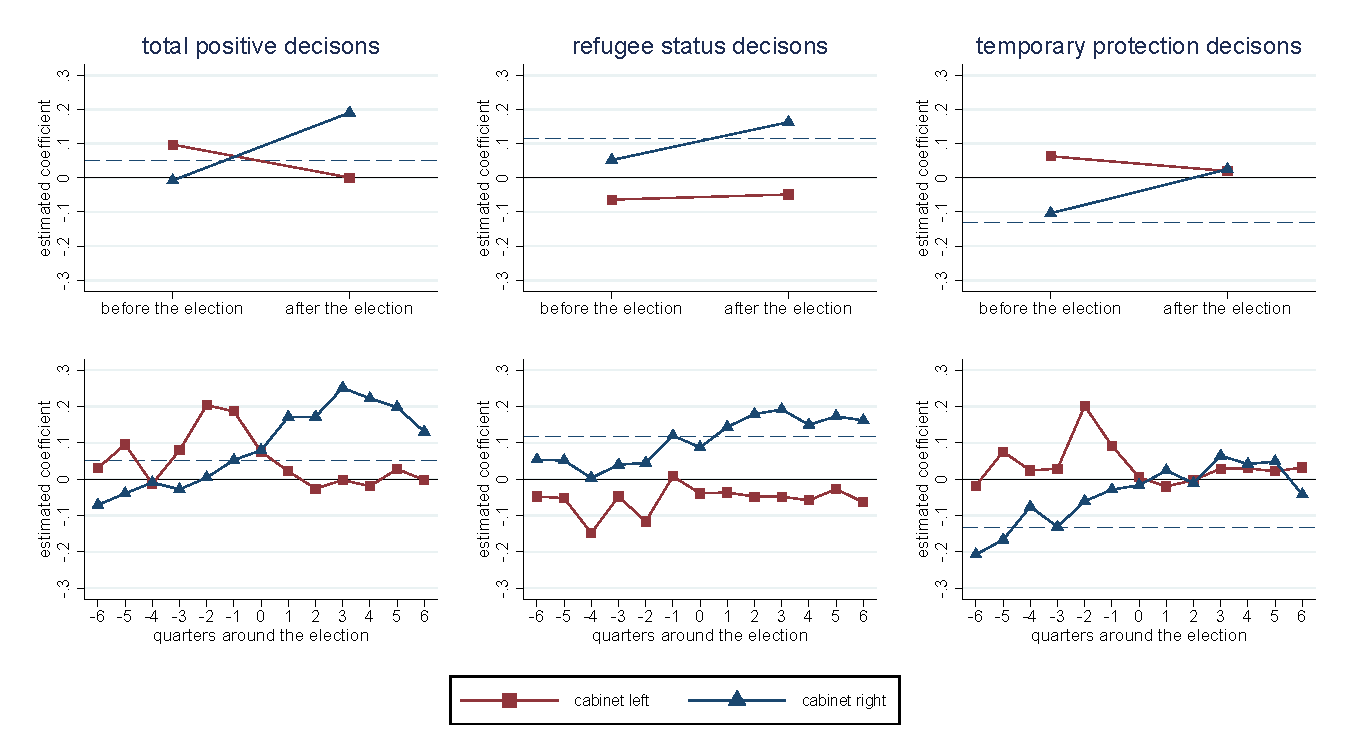
\includegraphics[width=\linewidth]{../results/decisions/dec_graphs_cabinet_right.pdf}
		{\scriptsize Note: These figures show the time evolution of positive decisions, refugee status decisions and temporary protection decisions as estimated in fixed effects regression with a set of dummies for before and after the election or a set of dummies for different quarters before and after an election in a quarter t = 0. Significant coefficients are indicated by filled plot markers. In addition to the controls that are specified in equation (XXX) in all decision regressions we control for the log of the total dyadic decisions per capita unless mentioned otherwise in the robustness checks.\par}
	\end{minipage}
\end{figure}

\begin{table}[htbp]\centering
\def\sym#1{\ifmmode^{#1}\else\(^{#1}\)\fi}
\caption{Coefficients quarterly model Decisions}
\begin{tabular}{l*{6}{c}}
\hline\hline
                    &\multicolumn{1}{c}{(1)}&\multicolumn{1}{c}{(2)}&\multicolumn{1}{c}{(3)}&\multicolumn{1}{c}{(4)}&\multicolumn{1}{c}{(5)}&\multicolumn{1}{c}{(6)}\\
                    &\multicolumn{1}{c}{left\_pos}&\multicolumn{1}{c}{right\_pos}&\multicolumn{1}{c}{left\_ref}&\multicolumn{1}{c}{right\_ref}&\multicolumn{1}{c}{left\_temp}&\multicolumn{1}{c}{right\_temp}\\
\hline
 6 quarters before the election&      0.0305         &      -0.123\sym{***}&     -0.0478         &     -0.0636\sym{**} &     -0.0179         &     -0.0756\sym{**} \\
                    &    (0.0266)         &    (0.0226)         &    (0.0315)         &    (0.0198)         &    (0.0359)         &    (0.0270)         \\
[1em]
 5 quarters before the election&      0.0957\sym{*}  &     -0.0910\sym{*}  &     -0.0521         &     -0.0660         &      0.0759         &     -0.0350         \\
                    &    (0.0413)         &    (0.0380)         &    (0.0350)         &    (0.0364)         &    (0.0391)         &    (0.0316)         \\
[1em]
 4 quarters before the election&     -0.0127         &     -0.0611         &      -0.148\sym{***}&      -0.114\sym{*}  &      0.0240         &      0.0563         \\
                    &    (0.0473)         &    (0.0393)         &    (0.0352)         &    (0.0447)         &    (0.0444)         &    (0.0339)         \\
[1em]
 3 quarters before the election&      0.0794         &     -0.0799         &     -0.0477         &     -0.0777         &      0.0290         &    0.000976         \\
                    &    (0.0423)         &    (0.0432)         &    (0.0343)         &    (0.0467)         &    (0.0443)         &    (0.0338)         \\
[1em]
 2 quarters before the election&       0.204\sym{***}&     -0.0474         &      -0.116\sym{***}&     -0.0722         &       0.202\sym{***}&      0.0714         \\
                    &    (0.0402)         &    (0.0467)         &    (0.0301)         &    (0.0411)         &    (0.0408)         &    (0.0452)         \\
[1em]
 1 quarters before the election&       0.187\sym{***}&    0.000985         &     0.00780         &     0.00244         &      0.0921\sym{*}  &       0.103\sym{*}  \\
                    &    (0.0518)         &    (0.0552)         &    (0.0370)         &    (0.0481)         &    (0.0466)         &    (0.0475)         \\
[1em]
Quarter of the election&      0.0755         &      0.0280         &     -0.0392         &     -0.0298         &     0.00525         &       0.115\sym{**} \\
                    &    (0.0426)         &    (0.0441)         &    (0.0395)         &    (0.0336)         &    (0.0395)         &    (0.0445)         \\
[1em]
 1 quarters after the election&      0.0217         &       0.120\sym{*}  &     -0.0364         &      0.0267         &     -0.0202         &       0.156\sym{***}\\
                    &    (0.0424)         &    (0.0480)         &    (0.0366)         &    (0.0337)         &    (0.0397)         &    (0.0464)         \\
[1em]
 2 quarters after the election&     -0.0259         &       0.120\sym{**} &     -0.0482         &      0.0618         &    -0.00226         &       0.121\sym{*}  \\
                    &    (0.0377)         &    (0.0451)         &    (0.0313)         &    (0.0368)         &    (0.0406)         &    (0.0478)         \\
[1em]
 3 quarters after the election&    -0.00234         &       0.200\sym{***}&     -0.0480         &      0.0746\sym{*}  &      0.0288         &       0.197\sym{***}\\
                    &    (0.0301)         &    (0.0351)         &    (0.0330)         &    (0.0350)         &    (0.0328)         &    (0.0440)         \\
[1em]
 4 quarters after the election&     -0.0194         &       0.170\sym{***}&     -0.0582\sym{*}  &      0.0322         &      0.0298         &       0.174\sym{***}\\
                    &    (0.0285)         &    (0.0363)         &    (0.0267)         &    (0.0451)         &    (0.0339)         &    (0.0395)         \\
[1em]
 5 quarters after the election&      0.0281         &       0.146\sym{***}&     -0.0271         &      0.0557         &      0.0218         &       0.181\sym{***}\\
                    &    (0.0350)         &    (0.0400)         &    (0.0338)         &    (0.0326)         &    (0.0380)         &    (0.0382)         \\
[1em]
 6 quarters after the election&    -0.00268         &      0.0784\sym{**} &     -0.0636\sym{*}  &      0.0443         &      0.0325         &      0.0898\sym{**} \\
                    &    (0.0330)         &    (0.0295)         &    (0.0316)         &    (0.0254)         &    (0.0274)         &    (0.0330)         \\
\hline
Observations        &       15938         &       15938         &       15938         &       15938         &       15938         &       15938         \\
\hline\hline
\multicolumn{7}{l}{\footnotesize Standard errors in parentheses}\\
\multicolumn{7}{l}{\footnotesize \sym{*} \(p<0.05\), \sym{**} \(p<0.01\), \sym{***} \(p<0.001\)}\\
\end{tabular}
\end{table}



% ================================================================================================================================================================

\clearpage
\FloatBarrier
\subsection{Robustness checks for positive decisions}

\begin{table}[htbp]\centering
\def\sym#1{\ifmmode^{#1}\else\(^{#1}\)\fi}
\caption{Determinats of log\_totalpositive\_pc}
\begin{tabular}{l*{6}{c}}
\hline\hline
                    &\multicolumn{1}{c}{(1)}&\multicolumn{1}{c}{(2)}&\multicolumn{1}{c}{(3)}&\multicolumn{1}{c}{(4)}&\multicolumn{1}{c}{(5)}&\multicolumn{1}{c}{(6)}\\
                    &\multicolumn{1}{c}{log\_totalpositive\_pc}&\multicolumn{1}{c}{log\_totalpositive\_pc}&\multicolumn{1}{c}{log\_totalpositive\_pc}&\multicolumn{1}{c}{log\_totalpositive\_pc}&\multicolumn{1}{c}{log\_totalpositive\_pc}&\multicolumn{1}{c}{log\_totalpositive\_pc}\\
\hline
Political Terror Scale&       0.283\sym{***}&                     &       0.283\sym{***}&       0.289\sym{***}&       0.289\sym{***}&       0.231\sym{***}\\
                    &    (0.0554)         &                     &    (0.0527)         &    (0.0545)         &    (0.0545)         &    (0.0571)         \\
[1em]
Civic Liberty (FHI) &       0.179         &                     &       0.175         &       0.195         &       0.195         &       0.197         \\
                    &     (0.113)         &                     &     (0.104)         &     (0.113)         &     (0.113)         &     (0.105)         \\
[1em]
Political Rights (FHI)&     -0.0295         &                     &     -0.0407         &     -0.0306         &     -0.0305         &     -0.0120         \\
                    &    (0.0584)         &                     &    (0.0563)         &    (0.0597)         &    (0.0596)         &    (0.0599)         \\
[1em]
Quarterly civil war battle death (000s)&       0.245\sym{***}&                     &       0.202\sym{***}&       0.243\sym{***}&       0.242\sym{***}&       0.247\sym{***}\\
                    &    (0.0311)         &                     &    (0.0296)         &    (0.0313)         &    (0.0313)         &    (0.0291)         \\
[1em]
Log origin country real GDP per capita&      -0.187         &                     &      -0.136         &      -0.211         &      -0.211         &      -0.160         \\
                    &     (0.120)         &                     &     (0.116)         &     (0.125)         &     (0.125)         &     (0.153)         \\
[1em]
Log destination country real GDP per capita&       0.274         &       0.237         &       0.511         &       0.363         &       0.358         &      -0.281         \\
                    &     (0.486)         &     (0.502)         &     (0.458)         &     (0.494)         &     (0.492)         &     (0.388)         \\
[1em]
Quarterly unemployment rate at destination&     -0.0330\sym{***}&     -0.0338\sym{***}&     -0.0176\sym{*}  &     -0.0309\sym{***}&     -0.0313\sym{***}&     -0.0236\sym{**} \\
                    &   (0.00758)         &   (0.00753)         &   (0.00774)         &   (0.00785)         &   (0.00777)         &   (0.00758)         \\
[1em]
Log average past total asylum decisions per capita&                     &                     &      1491.1\sym{***}&                     &                     &                     \\
                    &                     &                     &     (171.0)         &                     &                     &                     \\
[1em]
Log average past dyadic asylum decisions per capita&                     &                     &     13295.4\sym{***}&                     &                     &                     \\
                    &                     &                     &    (2953.5)         &                     &                     &                     \\
[1em]
after 2007          &                     &                     &                     &                     &       0.340         &                     \\
                    &                     &                     &                     &                     &     (0.170)         &                     \\
[1em]
Weighted cabinet position right&     -0.0425         &     -0.0278         &     -0.0801         &                     &     -0.0296         &     -0.0501         \\
                    &    (0.0481)         &    (0.0474)         &    (0.0440)         &                     &    (0.0462)         &    (0.0382)         \\
[1em]
Cabinet position left * Before the election&      0.0832\sym{**} &      0.0809\sym{*}  &      0.0779\sym{*}  &       0.104\sym{**} &      0.0882\sym{**} &    -0.00871         \\
                    &    (0.0304)         &    (0.0311)         &    (0.0298)         &    (0.0338)         &    (0.0294)         &    (0.0229)         \\
[1em]
Cabinet position left * After the election&      0.0548\sym{*}  &      0.0604\sym{**} &      0.0282         &      0.0688\sym{**} &      0.0531\sym{*}  &      0.0418\sym{*}  \\
                    &    (0.0217)         &    (0.0225)         &    (0.0207)         &    (0.0244)         &    (0.0215)         &    (0.0199)         \\
[1em]
Cabinet position right * Before the election&     -0.0248         &     -0.0288         &     -0.0179         &     -0.0395         &     -0.0267         &    -0.00907         \\
                    &    (0.0307)         &    (0.0308)         &    (0.0302)         &    (0.0274)         &    (0.0302)         &    (0.0231)         \\
[1em]
Cabinet position right * After the election&       0.139\sym{***}&       0.135\sym{***}&       0.179\sym{***}&       0.131\sym{***}&       0.144\sym{***}&      0.0538         \\
                    &    (0.0323)         &    (0.0321)         &    (0.0312)         &    (0.0263)         &    (0.0325)         &    (0.0315)         \\
\hline
Observations        &       15938         &       15938         &       15938         &       15938         &       15938         &       21955         \\
Adjusted \(R^{2}\)  &       0.432         &       0.437         &       0.178         &       0.130         &       0.130         &       0.119         \\
Fixed Effects       &           O         &       O x T         &       D x O         &       D x O         &       D x O         &       D x O         \\
Destination dummies &         Yes         &         Yes         &          No         &          No         &          No         &          No         \\
Quarter-Year dummies&         Yes         &          No         &         Yes         &         Yes         &         Yes         &         Yes         \\
\hline\hline
\multicolumn{7}{l}{\footnotesize Standard errors in parentheses}\\
\multicolumn{7}{l}{\footnotesize \sym{*} \(p<0.05\), \sym{**} \(p<0.01\), \sym{***} \(p<0.001\)}\\
\end{tabular}
\end{table}


\clearpage
\FloatBarrier
\begin{figure}[!ht]
	\caption{Total positive decisions per capita: predicted pattern - R1 to R6}
	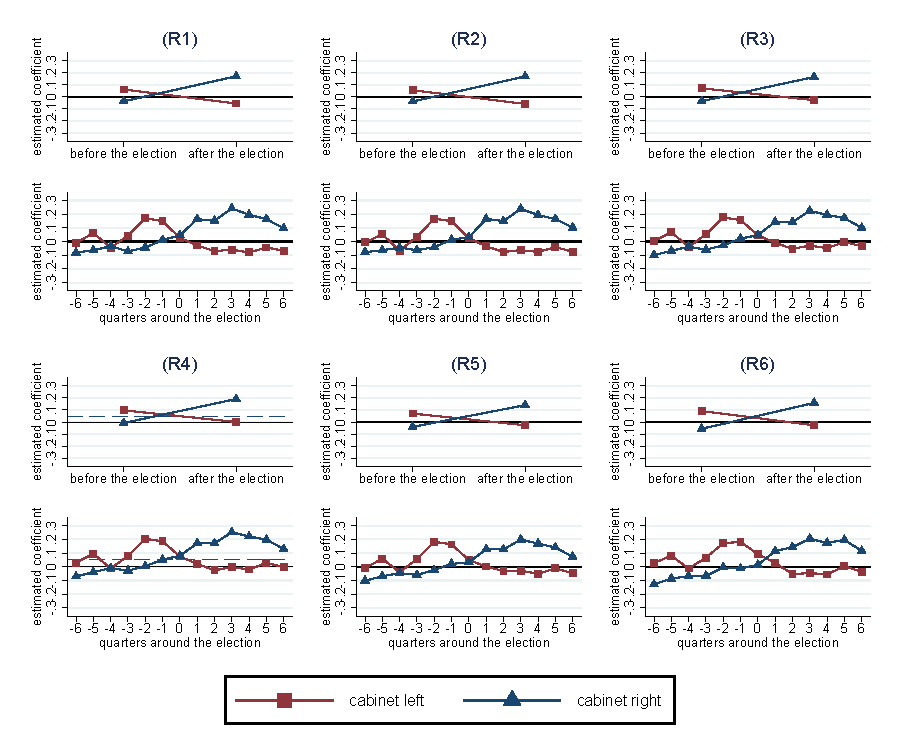
\includegraphics[width=1\textwidth]{../results/decisions/log_totalpositive_pc_graphs_R1-R6.pdf}
	\scriptsize{Note: These figures show the time evolution of positive decisions decisions as estimated in fixed effects regression with a set of dummies for before and after the election or a set of dummies for different quarters before and after an election in a quarter t = 0. Significant coefficients are indicated by filled plot markers.}
\end{figure}

\clearpage
\FloatBarrier

\begin{table}[htbp]\centering
\def\sym#1{\ifmmode^{#1}\else\(^{#1}\)\fi}
\caption{Coefficients quarterly model log\_totalpositive\_pc R1 - R3}
\begin{tabular}{l*{6}{c}}
\hline\hline
                    &\multicolumn{1}{c}{(1)}&\multicolumn{1}{c}{(2)}&\multicolumn{1}{c}{(3)}&\multicolumn{1}{c}{(4)}&\multicolumn{1}{c}{(5)}&\multicolumn{1}{c}{(6)}\\
                    &\multicolumn{1}{c}{left\_R1}&\multicolumn{1}{c}{right\_R1}&\multicolumn{1}{c}{left\_R2}&\multicolumn{1}{c}{right\_R2}&\multicolumn{1}{c}{left\_R3}&\multicolumn{1}{c}{right\_R3}\\
\hline
 6 quarters before the election&     -0.0103         &     -0.0804\sym{**} &    -0.00610         &     -0.0774\sym{**} &     0.00367         &     -0.0993\sym{***}\\
                    &    (0.0338)         &    (0.0291)         &    (0.0353)         &    (0.0292)         &    (0.0320)         &    (0.0290)         \\
[1em]
 5 quarters before the election&      0.0623         &     -0.0641         &      0.0527         &     -0.0638         &      0.0689         &     -0.0677         \\
                    &    (0.0431)         &    (0.0363)         &    (0.0453)         &    (0.0369)         &    (0.0435)         &    (0.0369)         \\
[1em]
 4 quarters before the election&     -0.0446         &     -0.0335         &     -0.0673         &     -0.0439         &     -0.0401         &     -0.0381         \\
                    &    (0.0538)         &    (0.0392)         &    (0.0528)         &    (0.0406)         &    (0.0535)         &    (0.0373)         \\
[1em]
 3 quarters before the election&      0.0419         &     -0.0721         &      0.0356         &     -0.0633         &      0.0532         &     -0.0586         \\
                    &    (0.0432)         &    (0.0475)         &    (0.0457)         &    (0.0488)         &    (0.0429)         &    (0.0443)         \\
[1em]
 2 quarters before the election&       0.171\sym{***}&     -0.0439         &       0.167\sym{***}&     -0.0401         &       0.177\sym{***}&     -0.0275         \\
                    &    (0.0433)         &    (0.0491)         &    (0.0448)         &    (0.0499)         &    (0.0429)         &    (0.0463)         \\
[1em]
 1 quarters before the election&       0.150\sym{**} &      0.0116         &       0.149\sym{**} &      0.0139         &       0.158\sym{**} &      0.0221         \\
                    &    (0.0541)         &    (0.0526)         &    (0.0537)         &    (0.0531)         &    (0.0531)         &    (0.0515)         \\
[1em]
Quarter of the election&      0.0271         &      0.0456         &      0.0249         &      0.0309         &      0.0461         &      0.0475         \\
                    &    (0.0458)         &    (0.0444)         &    (0.0461)         &    (0.0456)         &    (0.0449)         &    (0.0415)         \\
[1em]
 1 quarters after the election&     -0.0283         &       0.163\sym{***}&     -0.0349         &       0.166\sym{***}&    -0.00936         &       0.145\sym{**} \\
                    &    (0.0451)         &    (0.0490)         &    (0.0457)         &    (0.0493)         &    (0.0434)         &    (0.0460)         \\
[1em]
 2 quarters after the election&     -0.0698         &       0.153\sym{***}&     -0.0764         &       0.150\sym{***}&     -0.0530         &       0.143\sym{**} \\
                    &    (0.0393)         &    (0.0441)         &    (0.0411)         &    (0.0436)         &    (0.0374)         &    (0.0445)         \\
[1em]
 3 quarters after the election&     -0.0591         &       0.242\sym{***}&     -0.0626         &       0.239\sym{***}&     -0.0298         &       0.225\sym{***}\\
                    &    (0.0345)         &    (0.0343)         &    (0.0361)         &    (0.0348)         &    (0.0333)         &    (0.0326)         \\
[1em]
 4 quarters after the election&     -0.0793\sym{*}  &       0.196\sym{***}&     -0.0758\sym{*}  &       0.194\sym{***}&     -0.0479         &       0.195\sym{***}\\
                    &    (0.0347)         &    (0.0345)         &    (0.0352)         &    (0.0370)         &    (0.0348)         &    (0.0325)         \\
[1em]
 5 quarters after the election&     -0.0433         &       0.164\sym{***}&     -0.0405         &       0.164\sym{***}&    -0.00310         &       0.171\sym{***}\\
                    &    (0.0358)         &    (0.0420)         &    (0.0373)         &    (0.0429)         &    (0.0355)         &    (0.0402)         \\
[1em]
 6 quarters after the election&     -0.0671         &      0.0973\sym{**} &     -0.0738         &       0.102\sym{**} &     -0.0344         &       0.101\sym{***}\\
                    &    (0.0438)         &    (0.0306)         &    (0.0450)         &    (0.0313)         &    (0.0422)         &    (0.0294)         \\
\hline
Observations        &       15938         &       15938         &       15938         &       15938         &       15938         &       15938         \\
\hline\hline
\multicolumn{7}{l}{\footnotesize Standard errors in parentheses}\\
\multicolumn{7}{l}{\footnotesize \sym{*} \(p<0.05\), \sym{**} \(p<0.01\), \sym{***} \(p<0.001\)}\\
\end{tabular}
\end{table}

\begin{table}[htbp]\centering
\def\sym#1{\ifmmode^{#1}\else\(^{#1}\)\fi}
\caption{Coefficients log\_totalpositive\_pc R4 - R6}
\begin{tabular}{l*{6}{c}}
\hline\hline
                    &\multicolumn{1}{c}{(1)}&\multicolumn{1}{c}{(2)}&\multicolumn{1}{c}{(3)}&\multicolumn{1}{c}{(4)}&\multicolumn{1}{c}{(5)}&\multicolumn{1}{c}{(6)}\\
                    &\multicolumn{1}{c}{left\_R4}&\multicolumn{1}{c}{right\_R4}&\multicolumn{1}{c}{left\_R5}&\multicolumn{1}{c}{right\_R5}&\multicolumn{1}{c}{left\_R6}&\multicolumn{1}{c}{right\_R6}\\
\hline
 6 quarters before the election&      0.0505         &      -0.161\sym{***}&      0.0370         &      -0.150\sym{***}&     0.00358         &      -0.146\sym{***}\\
                    &    (0.0335)         &    (0.0323)         &    (0.0323)         &    (0.0284)         &    (0.0296)         &    (0.0198)         \\
[1em]
 5 quarters before the election&      0.0894         &     -0.0880\sym{*}  &      0.0759         &     -0.0766         &    -0.00617         &     -0.0354         \\
                    &    (0.0519)         &    (0.0432)         &    (0.0467)         &    (0.0447)         &    (0.0337)         &    (0.0375)         \\
[1em]
 4 quarters before the election&     -0.0200         &     -0.0589         &     -0.0330         &     -0.0477         &      -0.112\sym{**} &     -0.0328         \\
                    &    (0.0549)         &    (0.0377)         &    (0.0494)         &    (0.0413)         &    (0.0397)         &    (0.0369)         \\
[1em]
 3 quarters before the election&      0.0862         &     -0.0344         &      0.0733         &     -0.0239         &     -0.0455         &     -0.0245         \\
                    &    (0.0481)         &    (0.0437)         &    (0.0479)         &    (0.0424)         &    (0.0408)         &    (0.0378)         \\
[1em]
 2 quarters before the election&       0.201\sym{***}&      0.0112         &       0.188\sym{***}&      0.0221         &      0.0522         &     0.00160         \\
                    &    (0.0444)         &    (0.0455)         &    (0.0424)         &    (0.0471)         &    (0.0343)         &    (0.0371)         \\
[1em]
 1 quarters before the election&       0.182\sym{***}&      0.0567         &       0.167\sym{**} &      0.0679         &      0.0261         &       0.113\sym{**} \\
                    &    (0.0548)         &    (0.0545)         &    (0.0531)         &    (0.0563)         &    (0.0379)         &    (0.0354)         \\
[1em]
Quarter of the election&       0.100\sym{*}  &      0.0638         &      0.0858\sym{*}  &      0.0741         &     -0.0157         &      0.0837\sym{*}  \\
                    &    (0.0458)         &    (0.0438)         &    (0.0436)         &    (0.0508)         &    (0.0321)         &    (0.0367)         \\
[1em]
 1 quarters after the election&      0.0657         &      0.0727         &      0.0518         &      0.0835         &      0.0151         &     -0.0333         \\
                    &    (0.0435)         &    (0.0484)         &    (0.0429)         &    (0.0521)         &    (0.0348)         &    (0.0445)         \\
[1em]
 2 quarters after the election&     0.00905         &      0.0988\sym{*}  &    -0.00383         &       0.110\sym{*}  &     -0.0176         &     -0.0317         \\
                    &    (0.0369)         &    (0.0491)         &    (0.0398)         &    (0.0524)         &    (0.0307)         &    (0.0346)         \\
[1em]
 3 quarters after the election&      0.0678\sym{*}  &       0.160\sym{***}&      0.0550         &       0.171\sym{***}&      0.0451         &       0.105\sym{**} \\
                    &    (0.0315)         &    (0.0359)         &    (0.0314)         &    (0.0386)         &    (0.0304)         &    (0.0370)         \\
[1em]
 4 quarters after the election&      0.0547         &       0.173\sym{***}&      0.0412         &       0.184\sym{***}&      0.0369         &      0.0608         \\
                    &    (0.0335)         &    (0.0374)         &    (0.0289)         &    (0.0441)         &    (0.0278)         &    (0.0459)         \\
[1em]
 5 quarters after the election&       0.129\sym{***}&       0.173\sym{***}&       0.115\sym{**} &       0.184\sym{***}&       0.113\sym{***}&       0.135\sym{**} \\
                    &    (0.0375)         &    (0.0398)         &    (0.0362)         &    (0.0435)         &    (0.0324)         &    (0.0416)         \\
[1em]
 6 quarters after the election&      0.0726         &      0.0953\sym{**} &      0.0579         &       0.106\sym{**} &      0.0572\sym{*}  &      0.0826\sym{**} \\
                    &    (0.0376)         &    (0.0319)         &    (0.0305)         &    (0.0344)         &    (0.0258)         &    (0.0305)         \\
\hline
Observations        &       15938         &       15938         &       15938         &       15938         &       21955         &       21955         \\
\hline\hline
\multicolumn{7}{l}{\footnotesize Standard errors in parentheses}\\
\multicolumn{7}{l}{\footnotesize \sym{*} \(p<0.05\), \sym{**} \(p<0.01\), \sym{***} \(p<0.001\)}\\
\end{tabular}
\end{table}




\clearpage
\FloatBarrier
\begin{table}[htbp]\centering \scriptsize
\def\sym#1{\ifmmode^{#1}\else\(^{#1}\)\fi}
\caption{Determinats of positive decisions - R7 - R10}
\begin{tabular}{l*{4}{c}}
\hline\hline
                    &\multicolumn{1}{c}{(R7)}&\multicolumn{1}{c}{(R8)}&\multicolumn{1}{c}{(R9)}&\multicolumn{1}{c}{(R10)}\\
\hline
Political Terror Scale&       0.284\sym{***}&                     &       0.134\sym{**} &       0.134\sym{**} \\
                    &    (0.0564)         &                     &    (0.0423)         &    (0.0423)         \\
[0,5em]
Civic Liberty (FHI) &       0.186         &                     &       0.163\sym{*}  &       0.163\sym{*}  \\
                    &     (0.112)         &                     &    (0.0768)         &    (0.0768)         \\
[0,5em]
Political Rights (FHI)&     -0.0353         &                     &     -0.0246         &     -0.0246         \\
                    &    (0.0597)         &                     &    (0.0490)         &    (0.0490)         \\
[0,5em]
Quarterly civil war &       0.249\sym{***}&                     &       0.188\sym{***}&       0.188\sym{***}\\
battle death (000s)                    &    (0.0308)         &                     &    (0.0238)         &    (0.0238)         \\
[0,5em]
Log origin country real&      -0.179         &                     &     0.00171         &     0.00171         \\
 GDP per capita                    &     (0.122)         &                     &     (0.107)         &     (0.107)         \\
[0,5em]
Log destination country&       1.179\sym{*}  &       0.741\sym{*}  &      0.0235         &      0.0235         \\
 quarterly real GDP per capita                    &     (0.444)         &     (0.346)         &     (0.337)         &     (0.337)         \\
[0,5em]
Quarterly unemployment &     0.00239         &     -0.0134\sym{*}  &     -0.0180\sym{**} &     -0.0180\sym{**} \\
rate at destination                    &   (0.00709)         &   (0.00594)         &   (0.00568)         &   (0.00568)         \\
[0,5em]
Log total dyadic decisions&                     &       0.422\sym{***}&       0.342\sym{***}&       0.342\sym{***}\\
per capita                    &                     &    (0.0488)         &    (0.0358)         &    (0.0358)         \\
[0,5em]
Log total decisions at &       0.366\sym{***}&      0.0310         &                     &                     \\
destination per capita                    &    (0.0409)         &    (0.0288)         &                     &                     \\
[0,5em]
Years after 2007    &                     &                     &                     &       0.352\sym{*}  \\
                    &                     &                     &                     &     (0.141)         \\
[0,5em]
Cabinet position left *&      0.0641         &      0.0687\sym{*}  &      0.0197         &      0.0197         \\
 Before the election                    &    (0.0348)         &    (0.0320)         &    (0.0230)         &    (0.0230)         \\
[0,5em]
Cabinet position left * &      0.0153         &     -0.0339         &     0.00726         &     0.00726         \\
After the election                    &    (0.0260)         &    (0.0273)         &    (0.0225)         &    (0.0225)         \\
[0,5em]
Cabinet position right *&     -0.0453         &     -0.0394         &     -0.0254         &     -0.0254         \\
 Before the election                    &    (0.0278)         &    (0.0271)         &    (0.0198)         &    (0.0198)         \\
[0,5em]
Cabinet position right *&       0.141\sym{***}&       0.164\sym{***}&      0.0840\sym{***}&      0.0840\sym{***}\\
 After the election                    &    (0.0265)         &    (0.0254)         &    (0.0207)         &    (0.0207)         \\
\hline
Observations        &       15938         &       15938         &       21954         &       21954         \\
Adjusted \(R^{2}\)  &       0.160         &       0.272         &       0.283         &       0.283         \\
Fixed Effects       &       D x O         &       D x O         &       D x O         &       D x O         \\
Destination dummies &          No         &          No         &          No         &          No         \\
Quarter-Year dummies&         Yes         &         Yes         &         Yes         &         Yes         \\
\hline\hline
\multicolumn{5}{l}{Standard errors in parentheses \sym{*} \(p<0.05\), \sym{**} \(p<0.01\), \sym{***} \(p<0.001\)}\\
\end{tabular}
\end{table}


\clearpage
\FloatBarrier
\begin{figure}[!ht]
	\caption{Total positive decisions per capita: predicted pattern - R7 to R10}
	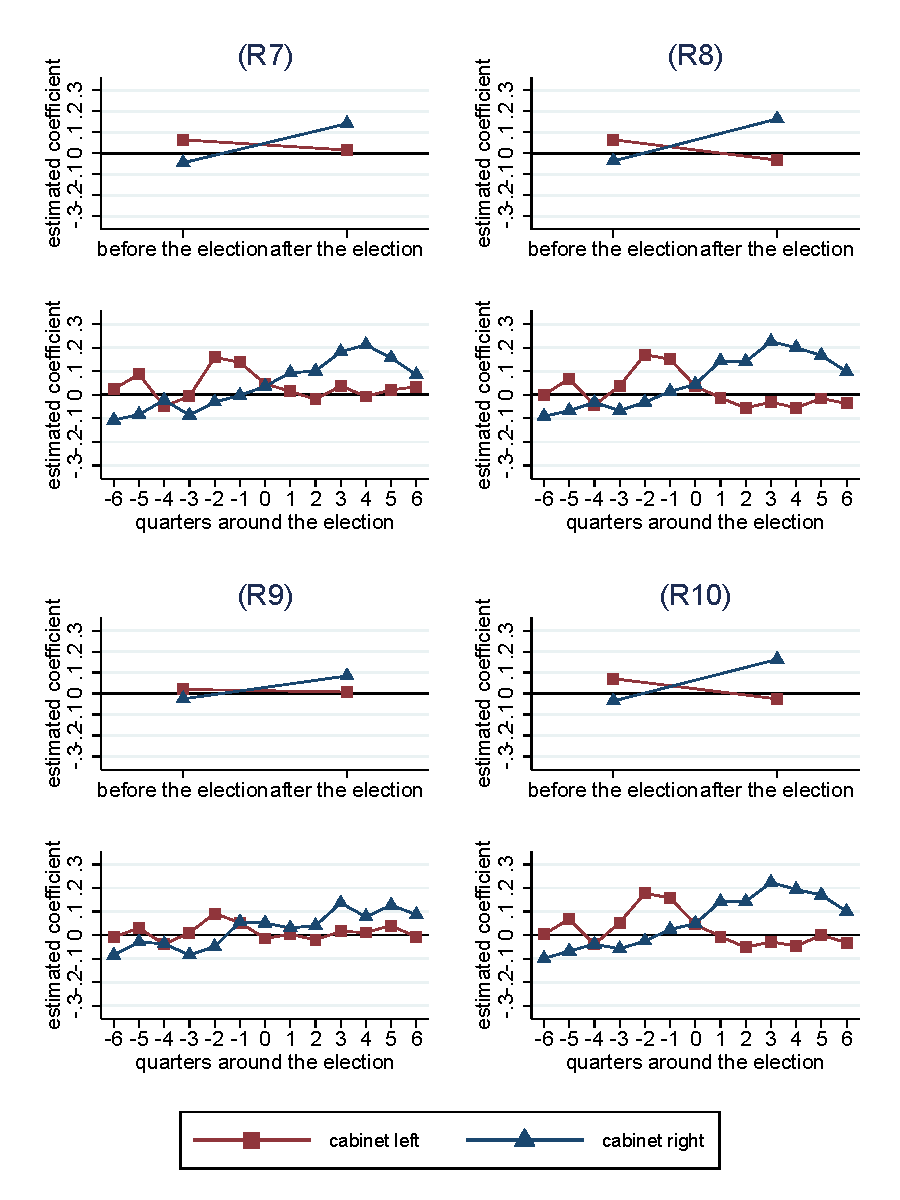
\includegraphics[width=1\textwidth]{../results/decisions/log_totalpositive_pc_graphs_R7-R10.pdf}
	\scriptsize{Note: These figures show the time evolution of positive decisions as estimated in fixed effects regression with a set of dummies for before and after the election or a set of dummies for different quarters before and after an election in a quarter t = 0. Significant coefficients are indicated by filled plot markers.}
\end{figure}

\begin{table}[htbp]\centering
\def\sym#1{\ifmmode^{#1}\else\(^{#1}\)\fi}
\caption{Coefficients quarterly model log\_totalpositive\_pc R7 - R10}
\begin{tabular}{l*{8}{c}}
\hline\hline
                    &\multicolumn{1}{c}{(1)}&\multicolumn{1}{c}{(2)}&\multicolumn{1}{c}{(3)}&\multicolumn{1}{c}{(4)}&\multicolumn{1}{c}{(5)}&\multicolumn{1}{c}{(6)}&\multicolumn{1}{c}{(7)}&\multicolumn{1}{c}{(8)}\\
                    &\multicolumn{1}{c}{left\_R7}&\multicolumn{1}{c}{right\_R7}&\multicolumn{1}{c}{left\_R8}&\multicolumn{1}{c}{right\_R8}&\multicolumn{1}{c}{left\_R9}&\multicolumn{1}{c}{right\_R9}&\multicolumn{1}{c}{left\_R10}&\multicolumn{1}{c}{right\_R10}\\
\hline
 6 quarters before the election&      0.0241         &      -0.107\sym{**} &   -0.000317         &     -0.0915\sym{**} &    -0.00843         &     -0.0853\sym{***}&     0.00309         &     -0.0993\sym{***}\\
                    &    (0.0354)         &    (0.0334)         &    (0.0320)         &    (0.0293)         &    (0.0267)         &    (0.0210)         &    (0.0319)         &    (0.0290)         \\
[1em]
 5 quarters before the election&      0.0871         &     -0.0836         &      0.0682         &     -0.0676         &      0.0298         &     -0.0292         &      0.0681         &     -0.0678         \\
                    &    (0.0519)         &    (0.0432)         &    (0.0438)         &    (0.0369)         &    (0.0309)         &    (0.0325)         &    (0.0437)         &    (0.0369)         \\
[1em]
 4 quarters before the election&     -0.0492         &     -0.0223         &     -0.0439         &     -0.0326         &     -0.0395         &     -0.0373         &     -0.0393         &     -0.0384         \\
                    &    (0.0561)         &    (0.0375)         &    (0.0532)         &    (0.0370)         &    (0.0375)         &    (0.0317)         &    (0.0533)         &    (0.0374)         \\
[1em]
 3 quarters before the election&    -0.00555         &     -0.0867         &      0.0380         &     -0.0668         &      0.0105         &     -0.0843\sym{*}  &      0.0531         &     -0.0583         \\
                    &    (0.0488)         &    (0.0455)         &    (0.0428)         &    (0.0444)         &    (0.0380)         &    (0.0361)         &    (0.0428)         &    (0.0443)         \\
[1em]
 2 quarters before the election&       0.159\sym{***}&     -0.0307         &       0.171\sym{***}&     -0.0315         &      0.0915\sym{**} &     -0.0493         &       0.177\sym{***}&     -0.0252         \\
                    &    (0.0455)         &    (0.0463)         &    (0.0427)         &    (0.0470)         &    (0.0318)         &    (0.0382)         &    (0.0425)         &    (0.0466)         \\
[1em]
 1 quarters before the election&       0.138\sym{*}  &    -0.00277         &       0.151\sym{**} &      0.0143         &      0.0524         &      0.0556         &       0.158\sym{**} &      0.0238         \\
                    &    (0.0552)         &    (0.0539)         &    (0.0531)         &    (0.0514)         &    (0.0372)         &    (0.0318)         &    (0.0529)         &    (0.0516)         \\
[1em]
Quarter of the election&      0.0467         &      0.0362         &      0.0380         &      0.0445         &     -0.0143         &      0.0510         &      0.0460         &      0.0489         \\
                    &    (0.0464)         &    (0.0451)         &    (0.0445)         &    (0.0418)         &    (0.0327)         &    (0.0307)         &    (0.0450)         &    (0.0415)         \\
[1em]
 1 quarters after the election&      0.0149         &      0.0936\sym{*}  &     -0.0135         &       0.144\sym{**} &     0.00323         &      0.0302         &    -0.00651         &       0.142\sym{**} \\
                    &    (0.0455)         &    (0.0476)         &    (0.0434)         &    (0.0476)         &    (0.0309)         &    (0.0370)         &    (0.0428)         &    (0.0478)         \\
[1em]
 2 quarters after the election&     -0.0197         &       0.101\sym{*}  &     -0.0556         &       0.141\sym{**} &     -0.0202         &      0.0401         &     -0.0521         &       0.142\sym{**} \\
                    &    (0.0374)         &    (0.0489)         &    (0.0375)         &    (0.0452)         &    (0.0289)         &    (0.0277)         &    (0.0374)         &    (0.0452)         \\
[1em]
 3 quarters after the election&      0.0380         &       0.183\sym{***}&     -0.0312         &       0.226\sym{***}&      0.0156         &       0.136\sym{***}&     -0.0284         &       0.224\sym{***}\\
                    &    (0.0313)         &    (0.0354)         &    (0.0336)         &    (0.0328)         &    (0.0309)         &    (0.0288)         &    (0.0339)         &    (0.0330)         \\
[1em]
 4 quarters after the election&    -0.00720         &       0.212\sym{***}&     -0.0549         &       0.200\sym{***}&      0.0112         &      0.0776\sym{**} &     -0.0467         &       0.194\sym{***}\\
                    &    (0.0347)         &    (0.0357)         &    (0.0347)         &    (0.0325)         &    (0.0324)         &    (0.0296)         &    (0.0348)         &    (0.0330)         \\
[1em]
 5 quarters after the election&      0.0211         &       0.157\sym{***}&     -0.0156         &       0.167\sym{***}&      0.0405         &       0.127\sym{***}&  -0.0000619         &       0.170\sym{***}\\
                    &    (0.0381)         &    (0.0407)         &    (0.0356)         &    (0.0401)         &    (0.0321)         &    (0.0336)         &    (0.0350)         &    (0.0399)         \\
[1em]
 6 quarters after the election&      0.0338         &      0.0848\sym{**} &     -0.0365         &      0.0985\sym{***}&    -0.00881         &      0.0867\sym{***}&     -0.0324         &       0.100\sym{***}\\
                    &    (0.0396)         &    (0.0320)         &    (0.0421)         &    (0.0294)         &    (0.0330)         &    (0.0220)         &    (0.0418)         &    (0.0293)         \\
\hline
Observations        &       15938         &       15938         &       15938         &       15938         &       21954         &       21954         &       15938         &       15938         \\
\hline\hline
\multicolumn{9}{l}{\footnotesize Standard errors in parentheses}\\
\multicolumn{9}{l}{\footnotesize \sym{*} \(p<0.05\), \sym{**} \(p<0.01\), \sym{***} \(p<0.001\)}\\
\end{tabular}
\end{table}



\clearpage
\FloatBarrier
\begin{table}[htbp]\centering \scriptsize
\def\sym#1{\ifmmode^{#1}\else\(^{#1}\)\fi}
\caption{Determinats of total positive decisions per capita - R11 - R16}
\begin{tabular}{l*{6}{c}}
\hline\hline
                    &\multicolumn{1}{c}{(R11)}&\multicolumn{1}{c}{(R12)}&\multicolumn{1}{c}{(R13)}&\multicolumn{1}{c}{(R14)}&\multicolumn{1}{c}{(R15)}&\multicolumn{1}{c}{(R16)}\\
\hline
Political Terror Scale&       0.284\sym{***}&       0.171\sym{***}&       0.173\sym{***}&       0.288\sym{***}&       0.196\sym{***}&       0.198\sym{***}\\
                    &    (0.0564)         &    (0.0350)         &    (0.0352)         &    (0.0565)         &    (0.0433)         &    (0.0435)         \\
[0,5em]
Civic Liberty (FHI) &       0.186         &       0.145         &       0.145         &       0.187         &       0.162         &       0.162         \\
                    &     (0.112)         &    (0.0830)         &    (0.0833)         &     (0.114)         &    (0.0890)         &    (0.0897)         \\
[0,5em]
Political Rights (FHI)&     -0.0348         &     -0.0433         &     -0.0435         &     -0.0330         &     -0.0483         &     -0.0483         \\
                    &    (0.0597)         &    (0.0498)         &    (0.0499)         &    (0.0604)         &    (0.0524)         &    (0.0526)         \\
[0,5em]
Quarterly civil war&       0.249\sym{***}&       0.185\sym{***}&       0.186\sym{***}&       0.248\sym{***}&       0.198\sym{***}&       0.200\sym{***}\\
 battle death (000s)                    &    (0.0308)         &    (0.0231)         &    (0.0240)         &    (0.0308)         &    (0.0302)         &    (0.0310)         \\
[0,5em]
Log origin country &      -0.182         &    -0.00536         &    -0.00619         &      -0.185         &     -0.0575         &     -0.0574         \\
real GDP per capita                    &     (0.122)         &    (0.0753)         &    (0.0759)         &     (0.124)         &    (0.0966)         &    (0.0973)         \\
[0,5em]
Log destination country &       1.053\sym{*}  &       0.501         &       0.556         &       0.931\sym{*}  &       0.676         &       0.758         \\
quarterly real GDP per capita                    &     (0.452)         &     (0.419)         &     (0.398)         &     (0.453)         &     (0.439)         &     (0.407)         \\
[0,5em]
Quarterly unemployment&    -0.00174         &     -0.0220\sym{**} &     -0.0197\sym{**} &    -0.00932         &     -0.0174\sym{*}  &     -0.0143\sym{*}  \\
 rate at destination                    &   (0.00719)         &   (0.00636)         &   (0.00632)         &   (0.00707)         &   (0.00658)         &   (0.00624)         \\
[0,5em]
Log total decisions at destination &       0.357\sym{***}&                     &      0.0297         &                     &                     &                     \\
per capita in previous year                    &    (0.0406)         &                     &    (0.0318)         &                     &                     &                     \\
[0,5em]
Log dyadic decisions at destination &                     &       0.403\sym{***}&       0.397\sym{***}&                     &                     &                     \\
per capita in previous year                    &                     &    (0.0417)         &    (0.0434)         &                     &                     &                     \\
[0,5em]
Log total first-time applications &                     &                     &                     &       0.230\sym{***}&                     &      0.0365         \\
in the previous 2 quarters                    &                     &                     &                     &    (0.0380)         &                     &    (0.0324)         \\
[0,5em]
Log dyadic first-time applications&                     &                     &                     &                     &       0.230\sym{***}&       0.224\sym{***}\\
 in the previous 2 quarters                    &                     &                     &                     &                     &    (0.0271)         &    (0.0273)         \\
[0,5em]
Cabinet position left *&      0.0782\sym{*}  &      0.0896\sym{*}  &      0.0877\sym{*}  &       0.101\sym{**} &      0.0960\sym{**} &      0.0956\sym{**} \\
 Before the election                    &    (0.0349)         &    (0.0352)         &    (0.0352)         &    (0.0342)         &    (0.0346)         &    (0.0347)         \\
[0,5em]
Cabinet position left * &      0.0201         &     -0.0190         &     -0.0217         &      0.0434         &      0.0131         &      0.0105         \\
After the election                    &    (0.0261)         &    (0.0283)         &    (0.0281)         &    (0.0259)         &    (0.0277)         &    (0.0277)         \\
[0,5em]
Cabinet position right *&     -0.0387         &     -0.0327         &     -0.0327         &     -0.0420         &     -0.0523         &     -0.0524         \\
 Before the election                    &    (0.0279)         &    (0.0267)         &    (0.0268)         &    (0.0277)         &    (0.0282)         &    (0.0282)         \\
[0,5em]
Cabinet position right *&       0.147\sym{***}&       0.177\sym{***}&       0.177\sym{***}&       0.143\sym{***}&       0.147\sym{***}&       0.149\sym{***}\\
 After the election                    &    (0.0264)         &    (0.0259)         &    (0.0257)         &    (0.0263)         &    (0.0282)         &    (0.0280)         \\
\hline
Observations        &       15938         &       15938         &       15938         &       15906         &       15882         &       15882         \\
Adjusted \(R^{2}\)  &       0.155         &       0.254         &       0.254         &       0.142         &       0.194         &       0.194         \\
Fixed Effects       &       D x O         &       D x O         &       D x O         &       D x O         &       D x O         &       D x O         \\
Destination dummies &          No         &          No         &          No         &          No         &          No         &          No         \\
Quarter-Year dummies&         Yes         &         Yes         &         Yes         &         Yes         &         Yes         &         Yes         \\
\hline\hline
\multicolumn{7}{l}{Standard errors in parentheses \sym{*} \(p<0.05\), \sym{**} \(p<0.01\), \sym{***} \(p<0.001\)}\\
\end{tabular}
\end{table}


\clearpage
\FloatBarrier
\begin{figure}[!ht]
	\caption{Total positive decisions per capita: predicted pattern - R11 to R16}
	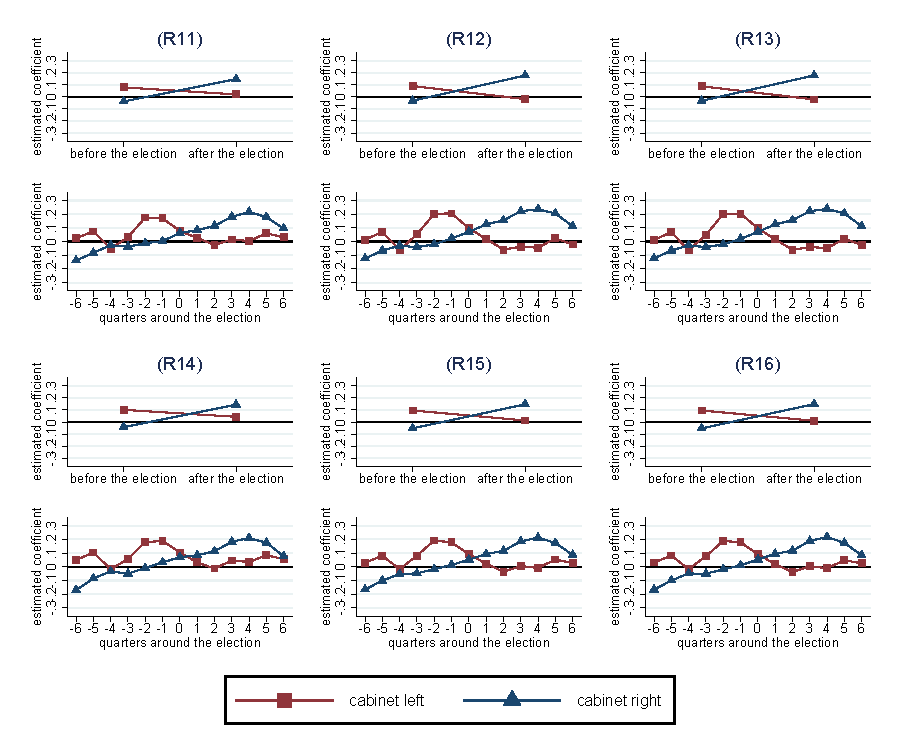
\includegraphics[width=1\textwidth]{../results/decisions/log_totalpositive_pc_graphs_R11-R16.pdf}
	\scriptsize{Note: These figures show the time evolution of positive decisions as estimated in fixed effects regression with a set of dummies for before and after the election or a set of dummies for different quarters before and after an election in a quarter t = 0. Significant coefficients are indicated by filled plot markers.}
\end{figure}

\clearpage
\FloatBarrier
\begin{table}[htbp]\centering
\def\sym#1{\ifmmode^{#1}\else\(^{#1}\)\fi}
\caption{Coefficients quarterly model log\_totalpositive\_pc R11 - R13}
\begin{tabular}{l*{6}{c}}
\hline\hline
                    &\multicolumn{1}{c}{(1)}&\multicolumn{1}{c}{(2)}&\multicolumn{1}{c}{(3)}&\multicolumn{1}{c}{(4)}&\multicolumn{1}{c}{(5)}&\multicolumn{1}{c}{(6)}\\
                    &\multicolumn{1}{c}{left\_R11}&\multicolumn{1}{c}{right\_R11}&\multicolumn{1}{c}{left\_R12}&\multicolumn{1}{c}{right\_R12}&\multicolumn{1}{c}{left\_R13}&\multicolumn{1}{c}{right\_R13}\\
\hline
 6 quarters before the election&      0.0251         &      -0.138\sym{***}&      0.0139         &      -0.124\sym{***}&      0.0124         &      -0.122\sym{***}\\
                    &    (0.0348)         &    (0.0330)         &    (0.0361)         &    (0.0295)         &    (0.0359)         &    (0.0296)         \\
[1em]
 5 quarters before the election&      0.0734         &     -0.0828         &      0.0700         &     -0.0658         &      0.0690         &     -0.0658         \\
                    &    (0.0520)         &    (0.0434)         &    (0.0481)         &    (0.0398)         &    (0.0483)         &    (0.0398)         \\
[1em]
 4 quarters before the election&     -0.0532         &     -0.0266         &     -0.0619         &     -0.0300         &     -0.0640         &     -0.0279         \\
                    &    (0.0563)         &    (0.0375)         &    (0.0559)         &    (0.0390)         &    (0.0556)         &    (0.0386)         \\
[1em]
 3 quarters before the election&      0.0320         &     -0.0379         &      0.0528         &     -0.0408         &      0.0490         &     -0.0410         \\
                    &    (0.0488)         &    (0.0442)         &    (0.0471)         &    (0.0425)         &    (0.0469)         &    (0.0426)         \\
[1em]
 2 quarters before the election&       0.176\sym{***}&     -0.0121         &       0.203\sym{***}&     -0.0192         &       0.201\sym{***}&     -0.0206         \\
                    &    (0.0456)         &    (0.0459)         &    (0.0452)         &    (0.0459)         &    (0.0454)         &    (0.0459)         \\
[1em]
 1 quarters before the election&       0.170\sym{**} &     0.00275         &       0.206\sym{***}&      0.0231         &       0.204\sym{***}&      0.0193         \\
                    &    (0.0551)         &    (0.0539)         &    (0.0580)         &    (0.0517)         &    (0.0582)         &    (0.0511)         \\
[1em]
Quarter of the election&      0.0775         &      0.0633         &      0.0982\sym{*}  &      0.0706         &      0.0964\sym{*}  &      0.0704         \\
                    &    (0.0460)         &    (0.0453)         &    (0.0461)         &    (0.0447)         &    (0.0459)         &    (0.0448)         \\
[1em]
 1 quarters after the election&      0.0261         &      0.0835         &      0.0186         &       0.126\sym{*}  &      0.0162         &       0.126\sym{*}  \\
                    &    (0.0450)         &    (0.0478)         &    (0.0447)         &    (0.0499)         &    (0.0450)         &    (0.0498)         \\
[1em]
 2 quarters after the election&     -0.0239         &       0.115\sym{*}  &     -0.0585         &       0.155\sym{**} &     -0.0601         &       0.156\sym{**} \\
                    &    (0.0377)         &    (0.0492)         &    (0.0393)         &    (0.0495)         &    (0.0391)         &    (0.0493)         \\
[1em]
 3 quarters after the election&      0.0151         &       0.181\sym{***}&     -0.0375         &       0.222\sym{***}&     -0.0402         &       0.223\sym{***}\\
                    &    (0.0317)         &    (0.0356)         &    (0.0369)         &    (0.0347)         &    (0.0360)         &    (0.0345)         \\
[1em]
 4 quarters after the election&     0.00382         &       0.217\sym{***}&     -0.0451         &       0.236\sym{***}&     -0.0476         &       0.238\sym{***}\\
                    &    (0.0348)         &    (0.0357)         &    (0.0376)         &    (0.0354)         &    (0.0373)         &    (0.0345)         \\
[1em]
 5 quarters after the election&      0.0605         &       0.179\sym{***}&      0.0238         &       0.206\sym{***}&      0.0199         &       0.206\sym{***}\\
                    &    (0.0379)         &    (0.0405)         &    (0.0363)         &    (0.0379)         &    (0.0364)         &    (0.0379)         \\
[1em]
 6 quarters after the election&      0.0306         &      0.0955\sym{**} &     -0.0213         &       0.112\sym{***}&     -0.0232         &       0.112\sym{***}\\
                    &    (0.0396)         &    (0.0319)         &    (0.0426)         &    (0.0296)         &    (0.0429)         &    (0.0296)         \\
\hline
Observations        &       15938         &       15938         &       15938         &       15938         &       15938         &       15938         \\
\hline\hline
\multicolumn{7}{l}{\footnotesize Standard errors in parentheses}\\
\multicolumn{7}{l}{\footnotesize \sym{*} \(p<0.05\), \sym{**} \(p<0.01\), \sym{***} \(p<0.001\)}\\
\end{tabular}
\end{table}

\begin{table}[htbp]\centering
\def\sym#1{\ifmmode^{#1}\else\(^{#1}\)\fi}
\caption{Coefficients quarterly model log\_totalpositive\_pc R14 - R16}
\begin{tabular}{l*{6}{c}}
\hline\hline
                    &\multicolumn{1}{c}{(1)}&\multicolumn{1}{c}{(2)}&\multicolumn{1}{c}{(3)}&\multicolumn{1}{c}{(4)}&\multicolumn{1}{c}{(5)}&\multicolumn{1}{c}{(6)}\\
                    &\multicolumn{1}{c}{left\_R14}&\multicolumn{1}{c}{right\_R14}&\multicolumn{1}{c}{left\_R15}&\multicolumn{1}{c}{right\_R15}&\multicolumn{1}{c}{left\_R16}&\multicolumn{1}{c}{right\_R16}\\
\hline
 6 quarters before the election&      0.0496         &      -0.170\sym{***}&      0.0309         &      -0.166\sym{***}&      0.0311         &      -0.167\sym{***}\\
                    &    (0.0339)         &    (0.0314)         &    (0.0349)         &    (0.0313)         &    (0.0349)         &    (0.0311)         \\
[1em]
 5 quarters before the election&       0.105\sym{*}  &     -0.0858\sym{*}  &      0.0805         &      -0.101\sym{*}  &      0.0829         &      -0.100\sym{*}  \\
                    &    (0.0516)         &    (0.0434)         &    (0.0519)         &    (0.0420)         &    (0.0515)         &    (0.0421)         \\
[1em]
 4 quarters before the election&     -0.0173         &     -0.0337         &     -0.0178         &     -0.0530         &     -0.0175         &     -0.0492         \\
                    &    (0.0548)         &    (0.0377)         &    (0.0525)         &    (0.0395)         &    (0.0525)         &    (0.0394)         \\
[1em]
 3 quarters before the election&      0.0563         &     -0.0504         &      0.0817         &     -0.0480         &      0.0771         &     -0.0501         \\
                    &    (0.0487)         &    (0.0442)         &    (0.0502)         &    (0.0441)         &    (0.0500)         &    (0.0442)         \\
[1em]
 2 quarters before the election&       0.181\sym{***}&    -0.00932         &       0.192\sym{***}&     -0.0166         &       0.189\sym{***}&     -0.0191         \\
                    &    (0.0467)         &    (0.0455)         &    (0.0467)         &    (0.0476)         &    (0.0473)         &    (0.0474)         \\
[1em]
 1 quarters before the election&       0.188\sym{***}&      0.0324         &       0.178\sym{**} &      0.0132         &       0.179\sym{**} &      0.0106         \\
                    &    (0.0554)         &    (0.0543)         &    (0.0571)         &    (0.0565)         &    (0.0570)         &    (0.0560)         \\
[1em]
Quarter of the election&       0.105\sym{*}  &      0.0703         &      0.0924\sym{*}  &      0.0517         &      0.0930\sym{*}  &      0.0530         \\
                    &    (0.0452)         &    (0.0453)         &    (0.0465)         &    (0.0477)         &    (0.0464)         &    (0.0480)         \\
[1em]
 1 quarters after the election&      0.0325         &      0.0844         &      0.0223         &      0.0929         &      0.0181         &      0.0943         \\
                    &    (0.0454)         &    (0.0478)         &    (0.0459)         &    (0.0509)         &    (0.0461)         &    (0.0504)         \\
[1em]
 2 quarters after the election&     -0.0130         &       0.114\sym{*}  &     -0.0358         &       0.117\sym{*}  &     -0.0378         &       0.118\sym{*}  \\
                    &    (0.0391)         &    (0.0492)         &    (0.0397)         &    (0.0495)         &    (0.0395)         &    (0.0492)         \\
[1em]
 3 quarters after the election&      0.0458         &       0.183\sym{***}&     0.00509         &       0.186\sym{***}&     0.00343         &       0.189\sym{***}\\
                    &    (0.0330)         &    (0.0354)         &    (0.0364)         &    (0.0374)         &    (0.0361)         &    (0.0371)         \\
[1em]
 4 quarters after the election&      0.0352         &       0.210\sym{***}&    -0.00869         &       0.213\sym{***}&     -0.0103         &       0.218\sym{***}\\
                    &    (0.0340)         &    (0.0353)         &    (0.0371)         &    (0.0382)         &    (0.0370)         &    (0.0376)         \\
[1em]
 5 quarters after the election&      0.0849\sym{*}  &       0.176\sym{***}&      0.0532         &       0.174\sym{***}&      0.0480         &       0.175\sym{***}\\
                    &    (0.0378)         &    (0.0403)         &    (0.0374)         &    (0.0418)         &    (0.0376)         &    (0.0418)         \\
[1em]
 6 quarters after the election&      0.0562         &      0.0775\sym{*}  &      0.0267         &      0.0867\sym{**} &      0.0251         &      0.0841\sym{**} \\
                    &    (0.0389)         &    (0.0313)         &    (0.0393)         &    (0.0318)         &    (0.0396)         &    (0.0314)         \\
\hline
Observations        &       15906         &       15906         &       15882         &       15882         &       15882         &       15882         \\
\hline\hline
\multicolumn{7}{l}{\footnotesize Standard errors in parentheses}\\
\multicolumn{7}{l}{\footnotesize \sym{*} \(p<0.05\), \sym{**} \(p<0.01\), \sym{***} \(p<0.001\)}\\
\end{tabular}
\end{table}



\clearpage
\FloatBarrier
\begin{table}[htbp]\centering
\def\sym#1{\ifmmode^{#1}\else\(^{#1}\)\fi}
\caption{Determinats of acceptance\_rate - R17 - R20}
\begin{tabular}{l*{4}{c}}
\hline\hline
                    &\multicolumn{1}{c}{(1)}&\multicolumn{1}{c}{(2)}&\multicolumn{1}{c}{(3)}&\multicolumn{1}{c}{(4)}\\
                    &\multicolumn{1}{c}{Acceptance rate}&\multicolumn{1}{c}{Acceptance rate}&\multicolumn{1}{c}{Acceptance rate}&\multicolumn{1}{c}{Acceptance rate}\\
\hline
Political Terror Scale&      0.0269\sym{*}  &                     &      0.0250\sym{*}  &      0.0256\sym{*}  \\
                    &    (0.0109)         &                     &    (0.0110)         &    (0.0108)         \\
[1em]
Civic Liberty (FHI) &      0.0345         &                     &      0.0345         &      0.0338         \\
                    &    (0.0226)         &                     &    (0.0221)         &    (0.0215)         \\
[1em]
Political Rights (FHI)&    -0.00792         &                     &    -0.00813         &    -0.00846         \\
                    &    (0.0199)         &                     &    (0.0199)         &    (0.0199)         \\
[1em]
Quarterly civil war battle death (000s)&      0.0532\sym{***}&                     &      0.0517\sym{***}&      0.0512\sym{***}\\
                    &   (0.00503)         &                     &   (0.00527)         &   (0.00581)         \\
[1em]
Log origin country real GDP per capita&     -0.0227         &                     &     -0.0210         &     -0.0222         \\
                    &    (0.0322)         &                     &    (0.0332)         &    (0.0332)         \\
[1em]
Log destination country quarterly real GDP per capita&       0.223\sym{*}  &       0.243\sym{**} &       0.189\sym{*}  &       0.204\sym{*}  \\
                    &    (0.0863)         &    (0.0899)         &    (0.0839)         &    (0.0912)         \\
[1em]
Quarterly unemployment rate at destination&  -0.0000658         &    0.000761         &    -0.00222         &   -0.000140         \\
                    &   (0.00115)         &   (0.00119)         &   (0.00141)         &   (0.00111)         \\
[1em]
Weighted cabinet position right&                     &      0.0370\sym{**} &                     &                     \\
                    &                     &    (0.0129)         &                     &                     \\
[1em]
Log total decisions at destination per capita in previous year&                     &                     &     -0.0315\sym{**} &                     \\
                    &                     &                     &    (0.0117)         &                     \\
[1em]
Log dyadic decisions at destination per capita in previous year&                     &                     &     0.00796         &                     \\
                    &                     &                     &   (0.00662)         &                     \\
[1em]
firsttimeapp\_total\_sum2&                     &                     &                     &-0.000000359         \\
                    &                     &                     &                     &(0.000000467)         \\
[1em]
firsttimeapp\_dyadic\_sum2&                     &                     &                     &   0.0000109         \\
                    &                     &                     &                     &(0.00000938)         \\
[1em]
Cabinet position left * Before the election&     0.00568         &      0.0274\sym{***}&     0.00674         &     0.00421         \\
                    &   (0.00771)         &   (0.00702)         &   (0.00766)         &   (0.00776)         \\
[1em]
Cabinet position left * After the election&     -0.0256\sym{**} &    -0.00578         &     -0.0236\sym{**} &     -0.0247\sym{**} \\
                    &   (0.00760)         &   (0.00665)         &   (0.00727)         &   (0.00717)         \\
[1em]
Cabinet position right * Before the election&     -0.0118         &     -0.0286\sym{**} &     -0.0124         &     -0.0116         \\
                    &   (0.00738)         &   (0.00838)         &   (0.00745)         &   (0.00742)         \\
[1em]
Cabinet position right * After the election&      0.0496\sym{***}&      0.0319\sym{***}&      0.0487\sym{***}&      0.0491\sym{***}\\
                    &   (0.00904)         &   (0.00750)         &   (0.00884)         &   (0.00907)         \\
\hline
Observations        &       12921         &       12921         &       12921         &       12868         \\
Adjusted \(R^{2}\)  &       0.134         &       0.081         &       0.137         &       0.133         \\
Fixed Effects       &       D x O         &       D x O         &       D x O         &       D x O         \\
Destination dummies &          No         &          No         &          No         &          No         \\
Quarter-Year dummies&         Yes         &         Yes         &         Yes         &         Yes         \\
\hline\hline
\multicolumn{5}{l}{\footnotesize Standard errors in parentheses}\\
\multicolumn{5}{l}{\footnotesize \sym{*} \(p<0.05\), \sym{**} \(p<0.01\), \sym{***} \(p<0.001\)}\\
\end{tabular}
\end{table}


\clearpage
\FloatBarrier
\begin{figure}[!ht]
	\caption{Acceptance rate: predicted pattern - R17 to R20}
	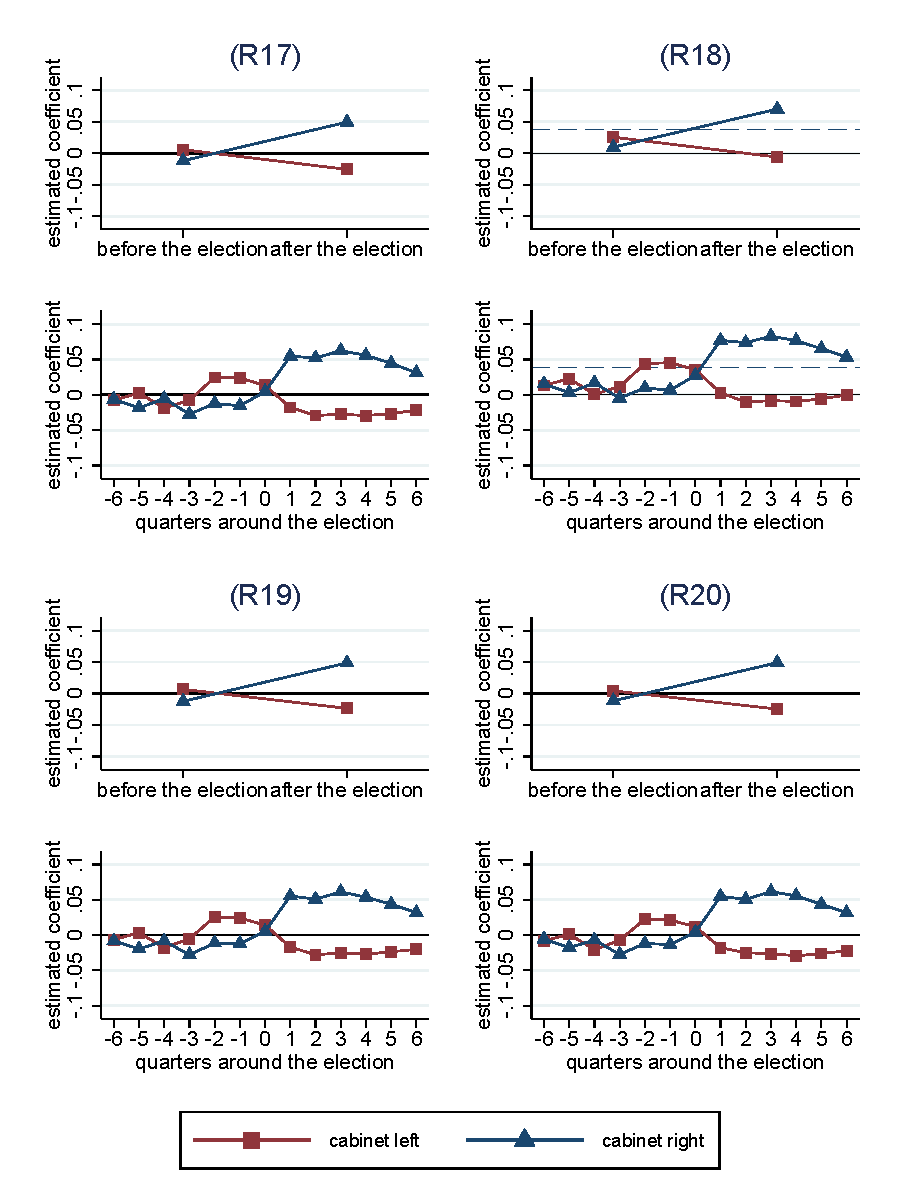
\includegraphics[width=1\textwidth]{../results/decisions/acceptance_rate_graphs_R17-R20.pdf}
	\scriptsize{Note: These figures show the time evolution of the share of positive decisions in all decisions made in that quarter in fixed effects regression with a set of dummies for before and after the election or a set of dummies for different quarters before and after an election in a quarter t = 0. Significant coefficients are indicated by filled plot markers.}
\end{figure}

\begin{table}[htbp]\centering
\def\sym#1{\ifmmode^{#1}\else\(^{#1}\)\fi}
\caption{Coefficients quarterly model acceptance\_rate R17 - R20}
\begin{tabular}{l*{8}{c}}
\hline\hline
                    &\multicolumn{1}{c}{(1)}&\multicolumn{1}{c}{(2)}&\multicolumn{1}{c}{(3)}&\multicolumn{1}{c}{(4)}&\multicolumn{1}{c}{(5)}&\multicolumn{1}{c}{(6)}&\multicolumn{1}{c}{(7)}&\multicolumn{1}{c}{(8)}\\
                    &\multicolumn{1}{c}{left\_R17}&\multicolumn{1}{c}{right\_R17}&\multicolumn{1}{c}{left\_R18}&\multicolumn{1}{c}{right\_R18}&\multicolumn{1}{c}{left\_R19}&\multicolumn{1}{c}{right\_R19}&\multicolumn{1}{c}{left\_R20}&\multicolumn{1}{c}{right\_R20}\\
\hline
 6 quarters before the election&    -0.00744         &    -0.00628         &      0.0132         &     -0.0228\sym{*}  &    -0.00644         &    -0.00828         &    -0.00802         &    -0.00569         \\
                    &   (0.00938)         &    (0.0115)         &   (0.00933)         &   (0.00964)         &   (0.00937)         &    (0.0113)         &   (0.00943)         &    (0.0115)         \\
[1em]
 5 quarters before the election&     0.00254         &     -0.0187         &      0.0229         &     -0.0353\sym{***}&     0.00339         &     -0.0196\sym{*}  &     0.00115         &     -0.0178         \\
                    &    (0.0132)         &   (0.00963)         &    (0.0128)         &   (0.00960)         &    (0.0131)         &   (0.00971)         &    (0.0134)         &   (0.00979)         \\
[1em]
 4 quarters before the election&     -0.0187         &    -0.00538         &    0.000794         &     -0.0214         &     -0.0179         &    -0.00830         &     -0.0205         &    -0.00689         \\
                    &    (0.0134)         &    (0.0113)         &    (0.0124)         &    (0.0115)         &    (0.0133)         &    (0.0115)         &    (0.0134)         &    (0.0115)         \\
[1em]
 3 quarters before the election&    -0.00749         &     -0.0275\sym{**} &      0.0117         &     -0.0429\sym{***}&    -0.00527         &     -0.0281\sym{**} &    -0.00737         &     -0.0274\sym{*}  \\
                    &    (0.0122)         &    (0.0106)         &    (0.0130)         &    (0.0123)         &    (0.0121)         &    (0.0107)         &    (0.0122)         &    (0.0109)         \\
[1em]
 2 quarters before the election&      0.0245\sym{*}  &     -0.0122         &      0.0440\sym{***}&     -0.0286\sym{*}  &      0.0259\sym{*}  &     -0.0112         &      0.0227\sym{*}  &     -0.0119         \\
                    &    (0.0111)         &    (0.0125)         &   (0.00972)         &    (0.0130)         &    (0.0110)         &    (0.0124)         &    (0.0112)         &    (0.0124)         \\
[1em]
 1 quarters before the election&      0.0237\sym{*}  &     -0.0155         &      0.0456\sym{***}&     -0.0317\sym{*}  &      0.0242\sym{*}  &     -0.0120         &      0.0213         &     -0.0134         \\
                    &    (0.0109)         &    (0.0145)         &    (0.0104)         &    (0.0154)         &    (0.0110)         &    (0.0143)         &    (0.0110)         &    (0.0142)         \\
[1em]
Quarter of the election&      0.0132         &     0.00437         &      0.0353\sym{**} &     -0.0110         &      0.0141         &     0.00518         &      0.0119         &     0.00377         \\
                    &    (0.0114)         &    (0.0129)         &    (0.0119)         &    (0.0156)         &    (0.0114)         &    (0.0127)         &    (0.0115)         &    (0.0124)         \\
[1em]
 1 quarters after the election&     -0.0179         &      0.0548\sym{**} &     0.00289         &      0.0388\sym{*}  &     -0.0170         &      0.0554\sym{**} &     -0.0178         &      0.0549\sym{**} \\
                    &    (0.0100)         &    (0.0178)         &   (0.00982)         &    (0.0169)         &   (0.00996)         &    (0.0178)         &    (0.0100)         &    (0.0178)         \\
[1em]
 2 quarters after the election&     -0.0293\sym{**} &      0.0521\sym{**} &     -0.0103         &      0.0355\sym{*}  &     -0.0279\sym{**} &      0.0509\sym{**} &     -0.0251\sym{*}  &      0.0505\sym{**} \\
                    &    (0.0108)         &    (0.0168)         &    (0.0109)         &    (0.0150)         &    (0.0106)         &    (0.0166)         &    (0.0105)         &    (0.0167)         \\
[1em]
 3 quarters after the election&     -0.0275\sym{**} &      0.0625\sym{***}&    -0.00822         &      0.0448\sym{***}&     -0.0252\sym{**} &      0.0611\sym{***}&     -0.0261\sym{**} &      0.0616\sym{***}\\
                    &   (0.00852)         &    (0.0130)         &   (0.00838)         &    (0.0110)         &   (0.00833)         &    (0.0128)         &   (0.00811)         &    (0.0130)         \\
[1em]
 4 quarters after the election&     -0.0293\sym{**} &      0.0558\sym{***}&    -0.00944         &      0.0385\sym{***}&     -0.0271\sym{**} &      0.0536\sym{***}&     -0.0294\sym{**} &      0.0555\sym{***}\\
                    &    (0.0102)         &   (0.00923)         &   (0.00844)         &   (0.00954)         &   (0.00990)         &   (0.00904)         &   (0.00974)         &   (0.00921)         \\
[1em]
 5 quarters after the election&     -0.0265\sym{*}  &      0.0446\sym{**} &    -0.00581         &      0.0270\sym{*}  &     -0.0235\sym{*}  &      0.0437\sym{**} &     -0.0260\sym{*}  &      0.0435\sym{**} \\
                    &    (0.0107)         &    (0.0145)         &   (0.00985)         &    (0.0122)         &    (0.0104)         &    (0.0142)         &    (0.0103)         &    (0.0146)         \\
[1em]
 6 quarters after the election&     -0.0218         &      0.0313\sym{**} &   -0.000134         &      0.0152         &     -0.0203         &      0.0317\sym{**} &     -0.0223         &      0.0316\sym{**} \\
                    &    (0.0129)         &    (0.0100)         &    (0.0126)         &    (0.0101)         &    (0.0127)         &   (0.00991)         &    (0.0131)         &    (0.0101)         \\
\hline
Observations        &       12921         &       12921         &       12921         &       12921         &       12921         &       12921         &       12868         &       12868         \\
\hline\hline
\multicolumn{9}{l}{\footnotesize Standard errors in parentheses}\\
\multicolumn{9}{l}{\footnotesize \sym{*} \(p<0.05\), \sym{**} \(p<0.01\), \sym{***} \(p<0.001\)}\\
\end{tabular}
\end{table}


% ================================================================================================================================================================
\clearpage
\FloatBarrier
\subsection{Robustness checks for refugee status decisions}

\begin{table}[!ht]\centering \scriptsize
\def\sym#1{\ifmmode^{#1}\else\(^{#1}\)\fi}
\caption{Determinats of refugee status decisions - R1 - R6}
\begin{tabular}{l*{6}{c}}
\hline\hline
                    &\multicolumn{1}{c}{(R1)}&\multicolumn{1}{c}{(R2)}&\multicolumn{1}{c}{(R3)}&\multicolumn{1}{c}{(R4)}&\multicolumn{1}{c}{(R5)}&\multicolumn{1}{c}{(R6)}\\
\hline
Political Terror Scale&       0.151\sym{***}&                     &       0.198\sym{***}&       0.196\sym{***}&       0.197\sym{***}&       0.200\sym{***}\\
                    &    (0.0417)         &                     &    (0.0463)         &    (0.0455)         &    (0.0455)         &    (0.0453)         \\
[0,5em]
Civic Liberty (FHI) &       0.188\sym{*}  &                     &       0.213\sym{*}  &       0.213\sym{*}  &       0.213\sym{*}  &       0.217\sym{*}  \\
                    &    (0.0908)         &                     &    (0.0967)         &    (0.0957)         &    (0.0959)         &    (0.0963)         \\
[0,5em]
Political Rights (FHI)&     -0.0550         &                     &     -0.0553         &     -0.0553         &     -0.0550         &     -0.0532         \\
                    &    (0.0562)         &                     &    (0.0607)         &    (0.0603)         &    (0.0601)         &    (0.0605)         \\
[0,5em]
Quarterly civil war&       0.115\sym{***}&                     &       0.136\sym{***}&       0.132\sym{***}&       0.133\sym{***}&       0.134\sym{***}\\
 battle death (000s)                    &    (0.0233)         &                     &    (0.0249)         &    (0.0248)         &    (0.0248)         &    (0.0247)         \\
[0,5em]
Log origin country&      0.0761         &                     &   0.0000903         &   -0.000760         &    -0.00327         &     0.00800         \\
 real GDP per capita                    &     (0.110)         &                     &     (0.117)         &     (0.116)         &     (0.116)         &     (0.115)         \\
[0,5em]
Log destination country&      -1.141\sym{**} &      -1.439\sym{***}&      -1.283\sym{**} &      -1.171\sym{**} &      -1.296\sym{**} &      -0.946\sym{**} \\
 quarterly real GDP per capita                    &     (0.367)         &     (0.370)         &     (0.413)         &     (0.391)         &     (0.396)         &     (0.345)         \\
[0,5em]
Quarterly unemployment&     -0.0306\sym{***}&     -0.0349\sym{***}&     -0.0338\sym{***}&     -0.0348\sym{***}&     -0.0371\sym{***}&     -0.0281\sym{***}\\
 rate at destination                    &   (0.00784)         &   (0.00811)         &   (0.00714)         &   (0.00737)         &   (0.00798)         &   (0.00767)         \\
[0,5em]
Log total dyadic decisions&       0.369\sym{***}&       0.374\sym{***}&       0.247\sym{***}&       0.257\sym{***}&       0.254\sym{***}&       0.253\sym{***}\\
per capita                    &    (0.0380)         &    (0.0370)         &    (0.0317)         &    (0.0338)         &    (0.0326)         &    (0.0320)         \\
[0,5em]
Log migrant stock in 2000/1&      0.0510\sym{**} &      0.0492\sym{**} &                     &                     &                     &                     \\
                    &    (0.0147)         &    (0.0145)         &                     &                     &                     &                     \\
[0,5em]
Log distance from origin&       0.472\sym{***}&       0.471\sym{***}&                     &                     &                     &                     \\
 to destination                    &     (0.133)         &     (0.133)         &                     &                     &                     &                     \\
[0,5em]
Log total average asylum applications&                     &                     &       0.120\sym{*}  &                     &                     &                     \\
 per capita in previous 5 years                    &                     &                     &    (0.0462)         &                     &                     &                     \\
[0,5em]
Asylum policy index overall&                     &                     &                     &                     &     -0.0116         &                     \\
                    &                     &                     &                     &                     &    (0.0119)         &                     \\
[0,5em]
Policy on access    &                     &                     &                     &                     &                     &     -0.0848\sym{**} \\
                    &                     &                     &                     &                     &                     &    (0.0276)         \\
[0,5em]
Policy on processing&                     &                     &                     &                     &                     &     -0.0209         \\
                    &                     &                     &                     &                     &                     &    (0.0195)         \\
[0,5em]
Policy on welfare   &                     &                     &                     &                     &                     &      0.0501\sym{**} \\
                    &                     &                     &                     &                     &                     &    (0.0181)         \\
[0,5em]
Cabinet position left *&      -0.132\sym{***}&      -0.137\sym{***}&      -0.125\sym{***}&     -0.0638\sym{**} &      -0.125\sym{***}&      -0.126\sym{***}\\
 Before the election                    &    (0.0297)         &    (0.0298)         &    (0.0291)         &    (0.0206)         &    (0.0291)         &    (0.0298)         \\
[0,5em]
Cabinet position left *&      -0.131\sym{***}&      -0.139\sym{***}&      -0.119\sym{***}&     -0.0489\sym{*}  &      -0.110\sym{***}&      -0.122\sym{***}\\
 After the election                    &    (0.0301)         &    (0.0320)         &    (0.0297)         &    (0.0204)         &    (0.0287)         &    (0.0288)         \\
[0,5em]
Cabinet position right *&     -0.0189         &     -0.0238         &     -0.0163         &     -0.0632\sym{*}  &     -0.0150         &     -0.0244         \\
 Before the election                    &    (0.0268)         &    (0.0291)         &    (0.0251)         &    (0.0274)         &    (0.0249)         &    (0.0241)         \\
[0,5em]
Cabinet position right *&      0.0965\sym{***}&       0.103\sym{***}&       0.104\sym{***}&      0.0478         &      0.0899\sym{***}&      0.0991\sym{***}\\
 After the election                    &    (0.0208)         &    (0.0223)         &    (0.0203)         &    (0.0249)         &    (0.0199)         &    (0.0198)         \\
\hline
Observations        &       15938         &       15938         &       15938         &       15938         &       15938         &       15938         \\
Adjusted \(R^{2}\)  &       0.550         &       0.554         &       0.230         &       0.228         &       0.228         &       0.233         \\
Fixed Effects       &           O         &       O x T         &       D x O         &       D x O         &       D x O         &       D x O         \\
Destination dummies &         Yes         &         Yes         &          No         &          No         &          No         &          No         \\
Quarter-Year dummies&         Yes         &          No         &         Yes         &         Yes         &         Yes         &         Yes         \\
\hline\hline
\multicolumn{7}{l}{Standard errors in parentheses \sym{*} \(p<0.05\), \sym{**} \(p<0.01\), \sym{***} \(p<0.001\)}\\
\end{tabular}
\end{table}


\clearpage
\FloatBarrier
\begin{figure}[!ht]
	\caption{Refugee status decisions per capita: predicted pattern - R1 to R6}
	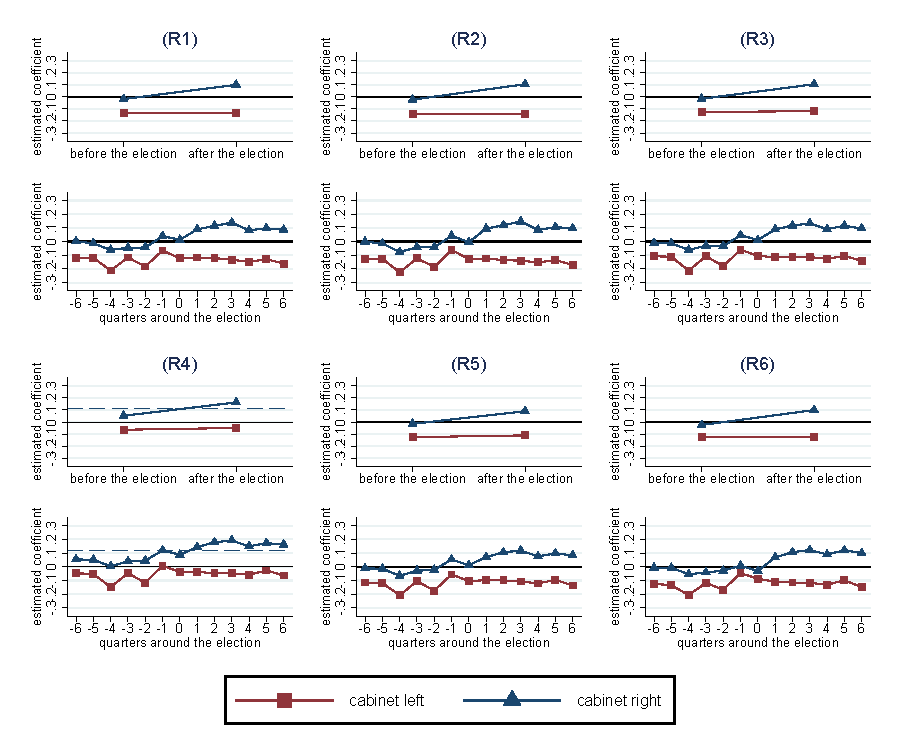
\includegraphics[width=1\textwidth]{../results/decisions/log_refugeestatus_pc_graphs_R1-R6.pdf}
	\scriptsize{Note: These figures show the time evolution of refugee status decisions decisions as estimated in fixed effects regression with a set of dummies for before and after the election or a set of dummies for different quarters before and after an election in a quarter t = 0. Significant coefficients are indicated by filled plot markers.}
\end{figure}

\clearpage
\FloatBarrier
\begin{table}[htbp]\centering
\def\sym#1{\ifmmode^{#1}\else\(^{#1}\)\fi}
\caption{Coefficients quarterly model log\_refugeestatus\_pc R1 - R3}
\begin{tabular}{l*{6}{c}}
\hline\hline
                    &\multicolumn{1}{c}{(1)}&\multicolumn{1}{c}{(2)}&\multicolumn{1}{c}{(3)}&\multicolumn{1}{c}{(4)}&\multicolumn{1}{c}{(5)}&\multicolumn{1}{c}{(6)}\\
                    &\multicolumn{1}{c}{left\_R1}&\multicolumn{1}{c}{right\_R1}&\multicolumn{1}{c}{left\_R2}&\multicolumn{1}{c}{right\_R2}&\multicolumn{1}{c}{left\_R3}&\multicolumn{1}{c}{right\_R3}\\
\hline
 6 quarters before the election&      -0.120\sym{**} &     0.00154         &      -0.126\sym{**} &    -0.00103         &      -0.107\sym{**} &     -0.0109         \\
                    &    (0.0409)         &    (0.0265)         &    (0.0408)         &    (0.0290)         &    (0.0385)         &    (0.0257)         \\
[1em]
 5 quarters before the election&      -0.119\sym{**} &     -0.0132         &      -0.125\sym{**} &     -0.0144         &      -0.111\sym{**} &     -0.0129         \\
                    &    (0.0394)         &    (0.0355)         &    (0.0383)         &    (0.0381)         &    (0.0378)         &    (0.0359)         \\
[1em]
 4 quarters before the election&      -0.212\sym{***}&     -0.0609         &      -0.225\sym{***}&     -0.0767         &      -0.212\sym{***}&     -0.0609         \\
                    &    (0.0454)         &    (0.0412)         &    (0.0454)         &    (0.0434)         &    (0.0442)         &    (0.0398)         \\
[1em]
 3 quarters before the election&      -0.116\sym{**} &     -0.0457         &      -0.123\sym{**} &     -0.0417         &      -0.107\sym{**} &     -0.0300         \\
                    &    (0.0378)         &    (0.0504)         &    (0.0397)         &    (0.0529)         &    (0.0368)         &    (0.0479)         \\
[1em]
 2 quarters before the election&      -0.182\sym{***}&     -0.0433         &      -0.186\sym{***}&     -0.0432         &      -0.180\sym{***}&     -0.0326         \\
                    &    (0.0405)         &    (0.0415)         &    (0.0408)         &    (0.0438)         &    (0.0408)         &    (0.0383)         \\
[1em]
 1 quarters before the election&     -0.0654         &      0.0406         &     -0.0610         &      0.0417         &     -0.0591         &      0.0463         \\
                    &    (0.0394)         &    (0.0447)         &    (0.0397)         &    (0.0476)         &    (0.0392)         &    (0.0437)         \\
[1em]
Quarter of the election&      -0.123\sym{**} &      0.0128         &      -0.128\sym{**} &    -0.00390         &      -0.105\sym{*}  &      0.0112         \\
                    &    (0.0425)         &    (0.0343)         &    (0.0439)         &    (0.0351)         &    (0.0413)         &    (0.0302)         \\
[1em]
 1 quarters after the election&      -0.117\sym{**} &      0.0892\sym{*}  &      -0.124\sym{**} &      0.0947\sym{*}  &      -0.113\sym{**} &      0.0888\sym{**} \\
                    &    (0.0400)         &    (0.0356)         &    (0.0426)         &    (0.0375)         &    (0.0405)         &    (0.0324)         \\
[1em]
 2 quarters after the election&      -0.120\sym{**} &       0.115\sym{***}&      -0.135\sym{**} &       0.120\sym{***}&      -0.112\sym{**} &       0.117\sym{***}\\
                    &    (0.0408)         &    (0.0333)         &    (0.0434)         &    (0.0351)         &    (0.0399)         &    (0.0339)         \\
[1em]
 3 quarters after the election&      -0.133\sym{***}&       0.138\sym{***}&      -0.140\sym{***}&       0.146\sym{***}&      -0.113\sym{**} &       0.132\sym{***}\\
                    &    (0.0353)         &    (0.0314)         &    (0.0363)         &    (0.0319)         &    (0.0360)         &    (0.0294)         \\
[1em]
 4 quarters after the election&      -0.148\sym{***}&      0.0819\sym{*}  &      -0.152\sym{***}&      0.0849\sym{*}  &      -0.126\sym{***}&      0.0907\sym{*}  \\
                    &    (0.0370)         &    (0.0368)         &    (0.0397)         &    (0.0382)         &    (0.0357)         &    (0.0353)         \\
[1em]
 5 quarters after the election&      -0.129\sym{***}&      0.0974\sym{**} &      -0.135\sym{***}&       0.106\sym{**} &      -0.105\sym{**} &       0.115\sym{***}\\
                    &    (0.0355)         &    (0.0334)         &    (0.0365)         &    (0.0360)         &    (0.0345)         &    (0.0336)         \\
[1em]
 6 quarters after the election&      -0.161\sym{***}&      0.0859\sym{**} &      -0.171\sym{***}&      0.0963\sym{**} &      -0.140\sym{**} &      0.0956\sym{***}\\
                    &    (0.0466)         &    (0.0309)         &    (0.0487)         &    (0.0330)         &    (0.0449)         &    (0.0290)         \\
\hline
Observations        &       15938         &       15938         &       15938         &       15938         &       15938         &       15938         \\
\hline\hline
\multicolumn{7}{l}{\footnotesize Standard errors in parentheses}\\
\multicolumn{7}{l}{\footnotesize \sym{*} \(p<0.05\), \sym{**} \(p<0.01\), \sym{***} \(p<0.001\)}\\
\end{tabular}
\end{table}

\begin{table}[htbp]\centering
\def\sym#1{\ifmmode^{#1}\else\(^{#1}\)\fi}
\caption{Coefficients quarterly model log\_refugeestatus\_pc R4 - R6}
\begin{tabular}{l*{6}{c}}
\hline\hline
                    &\multicolumn{1}{c}{(1)}&\multicolumn{1}{c}{(2)}&\multicolumn{1}{c}{(3)}&\multicolumn{1}{c}{(4)}&\multicolumn{1}{c}{(5)}&\multicolumn{1}{c}{(6)}\\
                    &\multicolumn{1}{c}{left\_R4}&\multicolumn{1}{c}{right\_R4}&\multicolumn{1}{c}{left\_R5}&\multicolumn{1}{c}{right\_R5}&\multicolumn{1}{c}{left\_R6}&\multicolumn{1}{c}{right\_R6}\\
\hline
 6 quarters before the election&     -0.0478         &     -0.0636\sym{**} &      -0.114\sym{**} &     -0.0118         &      -0.125\sym{**} &    -0.00691         \\
                    &    (0.0315)         &    (0.0198)         &    (0.0406)         &    (0.0254)         &    (0.0422)         &    (0.0252)         \\
[1em]
 5 quarters before the election&     -0.0521         &     -0.0660         &      -0.118\sym{**} &     -0.0139         &      -0.134\sym{**} &    -0.00763         \\
                    &    (0.0350)         &    (0.0364)         &    (0.0382)         &    (0.0356)         &    (0.0407)         &    (0.0368)         \\
[1em]
 4 quarters before the election&      -0.148\sym{***}&      -0.114\sym{*}  &      -0.209\sym{***}&     -0.0654         &      -0.207\sym{***}&     -0.0540         \\
                    &    (0.0352)         &    (0.0447)         &    (0.0439)         &    (0.0398)         &    (0.0441)         &    (0.0413)         \\
[1em]
 3 quarters before the election&     -0.0477         &     -0.0777         &      -0.106\sym{**} &     -0.0294         &      -0.118\sym{**} &     -0.0418         \\
                    &    (0.0343)         &    (0.0467)         &    (0.0368)         &    (0.0479)         &    (0.0371)         &    (0.0465)         \\
[1em]
 2 quarters before the election&      -0.116\sym{***}&     -0.0722         &      -0.174\sym{***}&     -0.0210         &      -0.167\sym{***}&     -0.0282         \\
                    &    (0.0301)         &    (0.0411)         &    (0.0391)         &    (0.0386)         &    (0.0390)         &    (0.0370)         \\
[1em]
 1 quarters before the election&     0.00780         &     0.00244         &     -0.0562         &      0.0532         &     -0.0465         &     0.00811         \\
                    &    (0.0370)         &    (0.0481)         &    (0.0381)         &    (0.0436)         &    (0.0379)         &    (0.0388)         \\
[1em]
Quarter of the election&     -0.0392         &     -0.0298         &      -0.105\sym{*}  &      0.0117         &     -0.0873\sym{*}  &     -0.0304         \\
                    &    (0.0395)         &    (0.0336)         &    (0.0411)         &    (0.0298)         &    (0.0417)         &    (0.0299)         \\
[1em]
 1 quarters after the election&     -0.0364         &      0.0267         &     -0.0973\sym{*}  &      0.0713\sym{*}  &      -0.110\sym{**} &      0.0687\sym{*}  \\
                    &    (0.0366)         &    (0.0337)         &    (0.0380)         &    (0.0312)         &    (0.0385)         &    (0.0309)         \\
[1em]
 2 quarters after the election&     -0.0482         &      0.0618         &     -0.0995\sym{**} &       0.106\sym{**} &      -0.115\sym{**} &       0.106\sym{**} \\
                    &    (0.0313)         &    (0.0368)         &    (0.0364)         &    (0.0335)         &    (0.0360)         &    (0.0340)         \\
[1em]
 3 quarters after the election&     -0.0480         &      0.0746\sym{*}  &      -0.107\sym{**} &       0.119\sym{***}&      -0.117\sym{***}&       0.122\sym{***}\\
                    &    (0.0330)         &    (0.0350)         &    (0.0354)         &    (0.0292)         &    (0.0352)         &    (0.0291)         \\
[1em]
 4 quarters after the election&     -0.0582\sym{*}  &      0.0322         &      -0.122\sym{***}&      0.0760\sym{*}  &      -0.131\sym{***}&      0.0906\sym{*}  \\
                    &    (0.0267)         &    (0.0451)         &    (0.0356)         &    (0.0378)         &    (0.0355)         &    (0.0368)         \\
[1em]
 5 quarters after the election&     -0.0271         &      0.0557         &     -0.0954\sym{**} &      0.0980\sym{**} &     -0.0982\sym{**} &       0.120\sym{***}\\
                    &    (0.0338)         &    (0.0326)         &    (0.0346)         &    (0.0329)         &    (0.0344)         &    (0.0331)         \\
[1em]
 6 quarters after the election&     -0.0636\sym{*}  &      0.0443         &      -0.137\sym{**} &      0.0839\sym{**} &      -0.150\sym{**} &      0.0998\sym{***}\\
                    &    (0.0316)         &    (0.0254)         &    (0.0464)         &    (0.0282)         &    (0.0476)         &    (0.0281)         \\
\hline
Observations        &       15938         &       15938         &       15938         &       15938         &       15938         &       15938         \\
\hline\hline
\multicolumn{7}{l}{\footnotesize Standard errors in parentheses}\\
\multicolumn{7}{l}{\footnotesize \sym{*} \(p<0.05\), \sym{**} \(p<0.01\), \sym{***} \(p<0.001\)}\\
\end{tabular}
\end{table}




\clearpage
\FloatBarrier
\begin{table}[!ht]\centering \scriptsize
\def\sym#1{\ifmmode^{#1}\else\(^{#1}\)\fi}
\caption{Determinats of refugee status decisions - R7 - R10}
\begin{tabular}{l*{4}{c}}
\hline\hline
                    &\multicolumn{1}{c}{(R7)}&\multicolumn{1}{c}{(R8)}&\multicolumn{1}{c}{(R9)}&\multicolumn{1}{c}{(R10)}\\

\hline
Political Terror Scale&       0.273\sym{***}&                     &       0.149\sym{**} &       0.149\sym{**} \\
                    &    (0.0609)         &                     &    (0.0490)         &    (0.0490)         \\
[0,5em]
Civic Liberty (FHI) &       0.243\sym{*}  &                     &       0.199\sym{*}  &       0.199\sym{*}  \\
                    &     (0.118)         &                     &    (0.0929)         &    (0.0929)         \\
[0,5em]
Political Rights (FHI)&     -0.0534         &                     &     -0.0404         &     -0.0404         \\
                    &    (0.0700)         &                     &    (0.0588)         &    (0.0588)         \\
[0,5em]
Quarterly civil war &       0.181\sym{***}&                     &       0.143\sym{***}&       0.143\sym{***}\\
battle death (000s)                    &    (0.0280)         &                     &    (0.0231)         &    (0.0231)         \\
[0,5em]
Log origin country &      -0.109         &                     &     -0.0250         &     -0.0250         \\
real GDP per capita                    &     (0.140)         &                     &     (0.149)         &     (0.149)         \\
[0,5em]
Log destination country&      -0.761         &      -1.032\sym{**} &      -1.058\sym{**} &      -1.058\sym{**} \\
 quarterly real GDP per capita                    &     (0.396)         &     (0.359)         &     (0.316)         &     (0.316)         \\
[0,5em]
Quarterly unemployment&     -0.0231\sym{**} &     -0.0334\sym{***}&     -0.0304\sym{***}&     -0.0304\sym{***}\\
 rate at destination                    &   (0.00674)         &   (0.00716)         &   (0.00644)         &   (0.00644)         \\
[0,5em]
Log total dyadic decisions&                     &       0.290\sym{***}&       0.211\sym{***}&       0.211\sym{***}\\
per capita                    &                     &    (0.0433)         &    (0.0280)         &    (0.0280)         \\
[0,5em]
Log total decisions at&       0.236\sym{***}&     0.00843         &                     &                     \\
 destination per capita                    &    (0.0433)         &    (0.0244)         &                     &                     \\
[0,5em]
Years after 2007    &                     &                     &                     &       0.518\sym{**} \\
                    &                     &                     &                     &     (0.193)         \\
[0,5em]
Cabinet position left *n&      -0.129\sym{***}&      -0.125\sym{***}&     -0.0946\sym{***}&     -0.0946\sym{***}\\
 Before the electio                    &    (0.0308)         &    (0.0299)         &    (0.0222)         &    (0.0222)         \\
[0,5em]
Cabinet position left *&     -0.0826\sym{**} &      -0.115\sym{***}&     -0.0669\sym{**} &     -0.0669\sym{**} \\
 After the election                    &    (0.0272)         &    (0.0294)         &    (0.0231)         &    (0.0231)         \\
[0,5em]
Cabinet position right *&     -0.0196         &     -0.0162         &     0.00594         &     0.00594         \\
  Before the election                   &    (0.0251)         &    (0.0252)         &    (0.0182)         &    (0.0182)         \\
[0,5em]
Cabinet position right *&      0.0841\sym{***}&      0.0984\sym{***}&      0.0507\sym{**} &      0.0507\sym{**} \\
 After the election                    &    (0.0214)         &    (0.0203)         &    (0.0159)         &    (0.0159)         \\
\hline
Observations        &       15938         &       15938         &       21952         &       21952         \\
Adjusted \(R^{2}\)  &       0.151         &       0.191         &       0.198         &       0.198         \\
Fixed Effects       &       D x O         &       D x O         &       D x O         &       D x O         \\
Destination dummies &          No         &          No         &          No         &          No         \\
Quarter-Year dummies&         Yes         &         Yes         &         Yes         &         Yes         \\
\hline\hline
\multicolumn{5}{l}{Standard errors in parentheses \sym{*} \(p<0.05\), \sym{**} \(p<0.01\), \sym{***} \(p<0.001\)}\\
\end{tabular}
\end{table}


\clearpage
\FloatBarrier
\begin{figure}[!ht]
	\caption{Refugee status decisions per capita: predicted pattern - R7 to R10}
	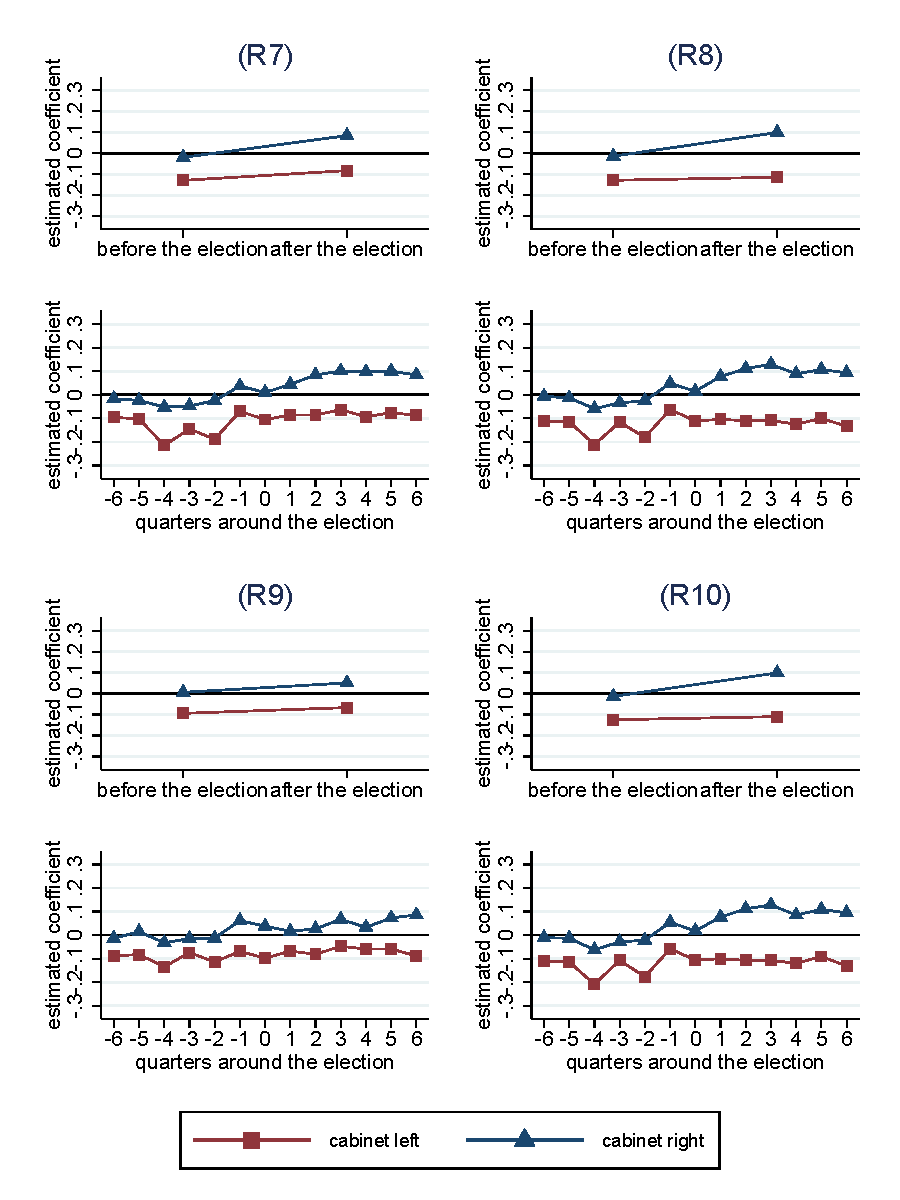
\includegraphics[width=1\textwidth]{../results/decisions/log_refugeestatus_pc_graphs_R7-R10.pdf}
	\scriptsize{Note: These figures show the time evolution of refugee status decisions as estimated in fixed effects regression with a set of dummies for before and after the election or a set of dummies for different quarters before and after an election in a quarter t = 0. Significant coefficients are indicated by filled plot markers.}
\end{figure}

\begin{table}[htbp]\centering
\def\sym#1{\ifmmode^{#1}\else\(^{#1}\)\fi}
\caption{Coefficients quarterly model log\_refugeestatus\_pc R7 - R10}
\begin{tabular}{l*{8}{c}}
\hline\hline
                    &\multicolumn{1}{c}{(1)}&\multicolumn{1}{c}{(2)}&\multicolumn{1}{c}{(3)}&\multicolumn{1}{c}{(4)}&\multicolumn{1}{c}{(5)}&\multicolumn{1}{c}{(6)}&\multicolumn{1}{c}{(7)}&\multicolumn{1}{c}{(8)}\\
                    &\multicolumn{1}{c}{left\_R7}&\multicolumn{1}{c}{right\_R7}&\multicolumn{1}{c}{left\_R8}&\multicolumn{1}{c}{right\_R8}&\multicolumn{1}{c}{left\_R9}&\multicolumn{1}{c}{right\_R9}&\multicolumn{1}{c}{left\_R10}&\multicolumn{1}{c}{right\_R10}\\
\hline
 6 quarters before the election&     -0.0958\sym{*}  &     -0.0167         &      -0.112\sym{**} &    -0.00623         &     -0.0881\sym{**} &     -0.0137         &      -0.110\sym{**} &     -0.0108         \\
                    &    (0.0391)         &    (0.0279)         &    (0.0394)         &    (0.0265)         &    (0.0314)         &    (0.0205)         &    (0.0391)         &    (0.0257)         \\
[1em]
 5 quarters before the election&      -0.102\sym{**} &     -0.0238         &      -0.115\sym{**} &     -0.0132         &     -0.0828\sym{**} &      0.0144         &      -0.115\sym{**} &     -0.0134         \\
                    &    (0.0384)         &    (0.0391)         &    (0.0381)         &    (0.0358)         &    (0.0289)         &    (0.0297)         &    (0.0382)         &    (0.0358)         \\
[1em]
 4 quarters before the election&      -0.215\sym{***}&     -0.0522         &      -0.211\sym{***}&     -0.0590         &      -0.135\sym{***}&     -0.0325         &      -0.209\sym{***}&     -0.0624         \\
                    &    (0.0438)         &    (0.0398)         &    (0.0442)         &    (0.0393)         &    (0.0331)         &    (0.0317)         &    (0.0439)         &    (0.0398)         \\
[1em]
 3 quarters before the election&      -0.145\sym{***}&     -0.0470         &      -0.116\sym{**} &     -0.0339         &     -0.0742\sym{*}  &     -0.0149         &      -0.107\sym{**} &     -0.0289         \\
                    &    (0.0429)         &    (0.0469)         &    (0.0388)         &    (0.0470)         &    (0.0301)         &    (0.0381)         &    (0.0369)         &    (0.0479)         \\
[1em]
 2 quarters before the election&      -0.188\sym{***}&     -0.0249         &      -0.181\sym{***}&     -0.0255         &      -0.114\sym{***}&     -0.0127         &      -0.177\sym{***}&     -0.0218         \\
                    &    (0.0431)         &    (0.0379)         &    (0.0410)         &    (0.0384)         &    (0.0264)         &    (0.0336)         &    (0.0402)         &    (0.0386)         \\
[1em]
 1 quarters before the election&     -0.0707         &      0.0374         &     -0.0624         &      0.0487         &     -0.0690\sym{*}  &      0.0615\sym{*}  &     -0.0584         &      0.0542         \\
                    &    (0.0424)         &    (0.0435)         &    (0.0398)         &    (0.0428)         &    (0.0282)         &    (0.0282)         &    (0.0390)         &    (0.0437)         \\
[1em]
Quarter of the election&      -0.105\sym{*}  &     0.00972         &      -0.111\sym{**} &      0.0152         &     -0.0981\sym{**} &      0.0373         &      -0.106\sym{*}  &      0.0178         \\
                    &    (0.0432)         &    (0.0289)         &    (0.0422)         &    (0.0301)         &    (0.0318)         &    (0.0226)         &    (0.0414)         &    (0.0305)         \\
[1em]
 1 quarters after the election&     -0.0858\sym{*}  &      0.0445         &      -0.104\sym{**} &      0.0776\sym{*}  &     -0.0679\sym{*}  &      0.0163         &      -0.100\sym{**} &      0.0765\sym{*}  \\
                    &    (0.0410)         &    (0.0309)         &    (0.0398)         &    (0.0319)         &    (0.0311)         &    (0.0236)         &    (0.0387)         &    (0.0320)         \\
[1em]
 2 quarters after the election&     -0.0858\sym{*}  &      0.0843\sym{*}  &      -0.110\sym{**} &       0.111\sym{**} &     -0.0816\sym{**} &      0.0264         &      -0.107\sym{**} &       0.111\sym{**} \\
                    &    (0.0387)         &    (0.0373)         &    (0.0396)         &    (0.0344)         &    (0.0313)         &    (0.0235)         &    (0.0394)         &    (0.0343)         \\
[1em]
 3 quarters after the election&     -0.0631         &       0.101\sym{***}&      -0.109\sym{**} &       0.129\sym{***}&     -0.0475         &      0.0668\sym{**} &      -0.107\sym{**} &       0.128\sym{***}\\
                    &    (0.0353)         &    (0.0289)         &    (0.0355)         &    (0.0294)         &    (0.0286)         &    (0.0228)         &    (0.0354)         &    (0.0295)         \\
[1em]
 4 quarters after the election&     -0.0933\sym{**} &      0.0969\sym{**} &      -0.125\sym{***}&      0.0889\sym{*}  &     -0.0590\sym{*}  &      0.0331         &      -0.120\sym{***}&      0.0852\sym{*}  \\
                    &    (0.0339)         &    (0.0356)         &    (0.0356)         &    (0.0346)         &    (0.0279)         &    (0.0283)         &    (0.0352)         &    (0.0358)         \\
[1em]
 5 quarters after the election&     -0.0759\sym{*}  &       0.100\sym{**} &      -0.100\sym{**} &       0.108\sym{**} &     -0.0594\sym{*}  &      0.0727\sym{**} &     -0.0910\sym{**} &       0.109\sym{***}\\
                    &    (0.0336)         &    (0.0337)         &    (0.0330)         &    (0.0332)         &    (0.0282)         &    (0.0253)         &    (0.0339)         &    (0.0330)         \\
[1em]
 6 quarters after the election&     -0.0870\sym{*}  &      0.0841\sym{**} &      -0.133\sym{**} &      0.0931\sym{**} &     -0.0882\sym{**} &      0.0856\sym{***}&      -0.131\sym{**} &      0.0943\sym{**} \\
                    &    (0.0413)         &    (0.0304)         &    (0.0444)         &    (0.0292)         &    (0.0309)         &    (0.0232)         &    (0.0441)         &    (0.0290)         \\
\hline
Observations        &       15938         &       15938         &       15938         &       15938         &       21952         &       21952         &       15938         &       15938         \\
\hline\hline
\multicolumn{9}{l}{\footnotesize Standard errors in parentheses}\\
\multicolumn{9}{l}{\footnotesize \sym{*} \(p<0.05\), \sym{**} \(p<0.01\), \sym{***} \(p<0.001\)}\\
\end{tabular}
\end{table}



\clearpage
\FloatBarrier
\begin{table}[!ht]\centering \scriptsize
\def\sym#1{\ifmmode^{#1}\else\(^{#1}\)\fi}
\caption{Determinats of refugee status decisions - R11 - R16}
\begin{tabular}{l*{6}{c}}
\hline\hline
                    &\multicolumn{1}{c}{(R11)}&\multicolumn{1}{c}{(R12)}&\multicolumn{1}{c}{(R13)}&\multicolumn{1}{c}{(R14)}&\multicolumn{1}{c}{(R15)}&\multicolumn{1}{c}{(R16)}\\
\hline
Political Terror Scale&       0.272\sym{***}&       0.194\sym{***}&       0.195\sym{***}&       0.274\sym{***}&       0.204\sym{***}&       0.207\sym{***}\\
                    &    (0.0609)         &    (0.0433)         &    (0.0440)         &    (0.0613)         &    (0.0490)         &    (0.0501)         \\
[0,5em]
Civic Liberty (FHI) &       0.243\sym{*}  &       0.215\sym{*}  &       0.215\sym{*}  &       0.243\sym{*}  &       0.225\sym{*}  &       0.224\sym{*}  \\
                    &     (0.118)         &    (0.0979)         &    (0.0982)         &     (0.119)         &     (0.101)         &     (0.102)         \\
[0,5em]
Political Rights (FHI)&     -0.0532         &     -0.0592         &     -0.0593         &     -0.0513         &     -0.0639         &     -0.0640         \\
                    &    (0.0699)         &    (0.0624)         &    (0.0626)         &    (0.0707)         &    (0.0631)         &    (0.0635)         \\
[0,5em]
Quarterly civil war &       0.182\sym{***}&       0.137\sym{***}&       0.138\sym{***}&       0.181\sym{***}&       0.142\sym{***}&       0.145\sym{***}\\
 battle death (000s)                   &    (0.0280)         &    (0.0244)         &    (0.0246)         &    (0.0280)         &    (0.0280)         &    (0.0284)         \\
[0,5em]
Log origin country&      -0.110         &      0.0132         &      0.0127         &      -0.109         &     -0.0124         &     -0.0122         \\
 real GDP per capita                    &     (0.140)         &     (0.117)         &     (0.117)         &     (0.141)         &     (0.125)         &     (0.126)         \\
[0,5em]
Log destination country&      -0.815         &      -1.193\sym{**} &      -1.161\sym{**} &      -0.791         &      -1.041\sym{*}  &      -0.931\sym{*}  \\
 quarterly real GDP per capita                    &     (0.406)         &     (0.408)         &     (0.379)         &     (0.402)         &     (0.420)         &     (0.382)         \\
[0,5em]
Quarterly unemployment&     -0.0247\sym{***}&     -0.0385\sym{***}&     -0.0372\sym{***}&     -0.0264\sym{***}&     -0.0345\sym{***}&     -0.0304\sym{***}\\
 rate at destination                    &   (0.00683)         &   (0.00791)         &   (0.00773)         &   (0.00657)         &   (0.00734)         &   (0.00635)         \\
[0,5em]
Log total decisions at destination&       0.245\sym{***}&                     &      0.0174         &                     &                     &                     \\
 per capita in previous year                    &    (0.0448)         &                     &    (0.0315)         &                     &                     &                     \\
[0,5em]
Log dyadic decisions at destination&                     &       0.280\sym{***}&       0.276\sym{***}&                     &                     &                     \\
  per capita in previous year                   &                     &    (0.0412)         &    (0.0408)         &                     &                     &                     \\
[0,5em]
Log total first-time applications&                     &                     &                     &       0.195\sym{***}&                     &      0.0493         \\
 in the previous 2 quarters                    &                     &                     &                     &    (0.0436)         &                     &    (0.0332)         \\
[0,5em]
Log dyadic first-time applications&                     &                     &                     &                     &       0.177\sym{***}&       0.169\sym{***}\\
 in the previous 2 quarters                    &                     &                     &                     &                     &    (0.0287)         &    (0.0272)         \\
[0,5em]
Cabinet position left * &      -0.121\sym{***}&      -0.113\sym{***}&      -0.114\sym{***}&      -0.105\sym{***}&      -0.109\sym{***}&      -0.109\sym{***}\\
Before the election                    &    (0.0301)         &    (0.0300)         &    (0.0304)         &    (0.0285)         &    (0.0280)         &    (0.0281)         \\
[0,5em]
Cabinet position left *&     -0.0814\sym{**} &      -0.109\sym{***}&      -0.110\sym{***}&     -0.0700\sym{*}  &     -0.0922\sym{**} &     -0.0958\sym{**} \\
 After the election                    &    (0.0271)         &    (0.0303)         &    (0.0304)         &    (0.0270)         &    (0.0287)         &    (0.0290)         \\
[0,5em]
Cabinet position right *&     -0.0152         &     -0.0111         &     -0.0111         &     -0.0184         &     -0.0264         &     -0.0265         \\
 Before the election                    &    (0.0255)         &    (0.0244)         &    (0.0244)         &    (0.0252)         &    (0.0244)         &    (0.0245)         \\
[0,5em]
Cabinet position right * &      0.0888\sym{***}&       0.109\sym{***}&       0.110\sym{***}&      0.0879\sym{***}&      0.0900\sym{***}&      0.0921\sym{***}\\
After the election                    &    (0.0212)         &    (0.0214)         &    (0.0212)         &    (0.0213)         &    (0.0221)         &    (0.0218)         \\
\hline
Observations        &       15938         &       15938         &       15938         &       15906         &       15882         &       15882         \\
Adjusted \(R^{2}\)  &       0.150         &       0.208         &       0.208         &       0.146         &       0.183         &       0.183         \\
Fixed Effects       &       D x O         &       D x O         &       D x O         &       D x O         &       D x O         &       D x O         \\
Destination dummies &          No         &          No         &          No         &          No         &          No         &          No         \\
Quarter-Year dummies&         Yes         &         Yes         &         Yes         &         Yes         &         Yes         &         Yes         \\
\hline\hline
\multicolumn{7}{l}{Standard errors in parentheses \sym{*} \(p<0.05\), \sym{**} \(p<0.01\), \sym{***} \(p<0.001\)}\\
\end{tabular}
\end{table}


\clearpage
\FloatBarrier
\begin{figure}[!ht]
	\caption{Refugee status decisions per capita: predicted pattern - R11 to R16}
	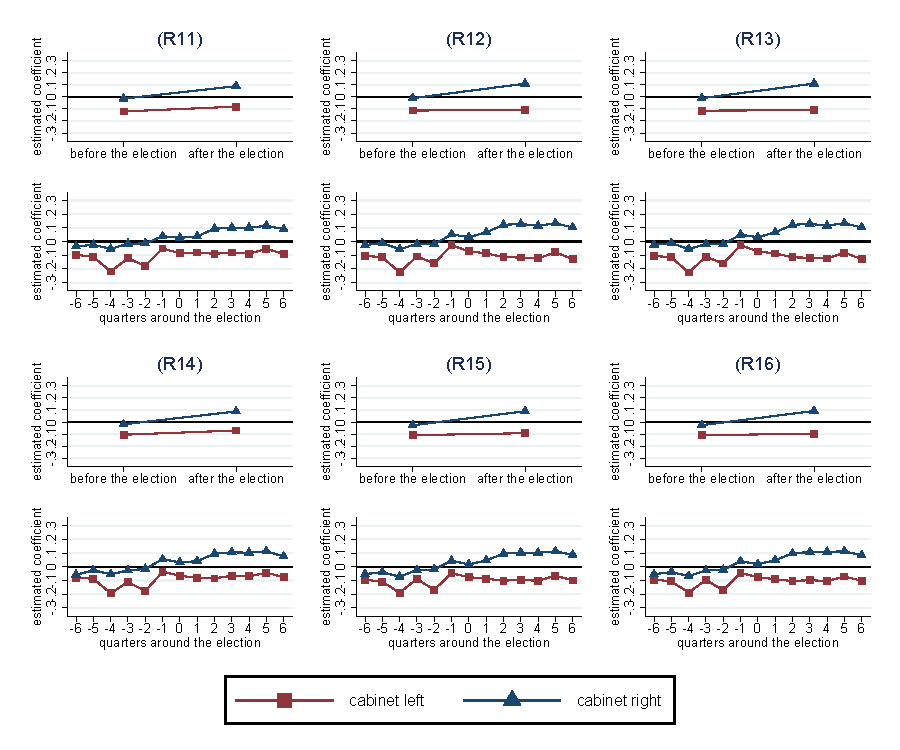
\includegraphics[width=1\textwidth]{../results/decisions/log_refugeestatus_pc_graphs_R11-R16.pdf}
	\scriptsize{Note: These figures show the time evolution of refugee status decisions as estimated in fixed effects regression with a set of dummies for before and after the election or a set of dummies for different quarters before and after an election in a quarter t = 0. Significant coefficients are indicated by filled plot markers.}
\end{figure}

\clearpage
\FloatBarrier
\begin{table}[htbp]\centering
\def\sym#1{\ifmmode^{#1}\else\(^{#1}\)\fi}
\caption{Coefficients quarterly model log\_refugeestatus\_pc R11 - R13}
\begin{tabular}{l*{6}{c}}
\hline\hline
                    &\multicolumn{1}{c}{(1)}&\multicolumn{1}{c}{(2)}&\multicolumn{1}{c}{(3)}&\multicolumn{1}{c}{(4)}&\multicolumn{1}{c}{(5)}&\multicolumn{1}{c}{(6)}\\
                    &\multicolumn{1}{c}{left\_R11}&\multicolumn{1}{c}{right\_R11}&\multicolumn{1}{c}{left\_R12}&\multicolumn{1}{c}{right\_R12}&\multicolumn{1}{c}{left\_R13}&\multicolumn{1}{c}{right\_R13}\\
\hline
 6 quarters before the election&     -0.0961\sym{*}  &     -0.0359         &      -0.104\sym{**} &     -0.0255         &      -0.105\sym{**} &     -0.0248         \\
                    &    (0.0390)         &    (0.0274)         &    (0.0398)         &    (0.0239)         &    (0.0400)         &    (0.0241)         \\
[1em]
 5 quarters before the election&      -0.112\sym{**} &     -0.0231         &      -0.114\sym{**} &     -0.0113         &      -0.115\sym{**} &     -0.0112         \\
                    &    (0.0391)         &    (0.0393)         &    (0.0389)         &    (0.0370)         &    (0.0390)         &    (0.0371)         \\
[1em]
 4 quarters before the election&      -0.219\sym{***}&     -0.0538         &      -0.225\sym{***}&     -0.0559         &      -0.226\sym{***}&     -0.0547         \\
                    &    (0.0441)         &    (0.0398)         &    (0.0453)         &    (0.0411)         &    (0.0454)         &    (0.0406)         \\
[1em]
 3 quarters before the election&      -0.123\sym{**} &     -0.0156         &      -0.109\sym{**} &     -0.0176         &      -0.111\sym{**} &     -0.0177         \\
                    &    (0.0414)         &    (0.0478)         &    (0.0381)         &    (0.0452)         &    (0.0388)         &    (0.0452)         \\
[1em]
 2 quarters before the election&      -0.178\sym{***}&     -0.0138         &      -0.159\sym{***}&     -0.0189         &      -0.161\sym{***}&     -0.0197         \\
                    &    (0.0425)         &    (0.0385)         &    (0.0417)         &    (0.0374)         &    (0.0419)         &    (0.0373)         \\
[1em]
 1 quarters before the election&     -0.0508         &      0.0390         &     -0.0260         &      0.0526         &     -0.0267         &      0.0505         \\
                    &    (0.0411)         &    (0.0438)         &    (0.0412)         &    (0.0437)         &    (0.0415)         &    (0.0429)         \\
[1em]
Quarter of the election&     -0.0858\sym{*}  &      0.0272         &     -0.0718         &      0.0322         &     -0.0727         &      0.0321         \\
                    &    (0.0417)         &    (0.0301)         &    (0.0418)         &    (0.0307)         &    (0.0419)         &    (0.0307)         \\
[1em]
 1 quarters after the election&     -0.0800\sym{*}  &      0.0383         &     -0.0855\sym{*}  &      0.0677\sym{*}  &     -0.0869\sym{*}  &      0.0677\sym{*}  \\
                    &    (0.0404)         &    (0.0310)         &    (0.0394)         &    (0.0313)         &    (0.0401)         &    (0.0313)         \\
[1em]
 2 quarters after the election&     -0.0898\sym{*}  &      0.0941\sym{*}  &      -0.114\sym{**} &       0.122\sym{***}&      -0.115\sym{**} &       0.122\sym{***}\\
                    &    (0.0390)         &    (0.0371)         &    (0.0409)         &    (0.0369)         &    (0.0409)         &    (0.0368)         \\
[1em]
 3 quarters after the election&     -0.0799\sym{*}  &       0.101\sym{***}&      -0.117\sym{**} &       0.129\sym{***}&      -0.118\sym{**} &       0.129\sym{***}\\
                    &    (0.0361)         &    (0.0290)         &    (0.0395)         &    (0.0284)         &    (0.0394)         &    (0.0283)         \\
[1em]
 4 quarters after the election&     -0.0881\sym{**} &       0.101\sym{**} &      -0.122\sym{**} &       0.115\sym{**} &      -0.124\sym{***}&       0.117\sym{***}\\
                    &    (0.0334)         &    (0.0353)         &    (0.0375)         &    (0.0367)         &    (0.0376)         &    (0.0353)         \\
[1em]
 5 quarters after the election&     -0.0530         &       0.115\sym{***}&     -0.0790\sym{*}  &       0.134\sym{***}&     -0.0812\sym{*}  &       0.134\sym{***}\\
                    &    (0.0328)         &    (0.0337)         &    (0.0343)         &    (0.0332)         &    (0.0333)         &    (0.0332)         \\
[1em]
 6 quarters after the election&     -0.0906\sym{*}  &      0.0910\sym{**} &      -0.127\sym{**} &       0.103\sym{***}&      -0.128\sym{**} &       0.103\sym{***}\\
                    &    (0.0416)         &    (0.0304)         &    (0.0449)         &    (0.0305)         &    (0.0450)         &    (0.0306)         \\
\hline
Observations        &       15938         &       15938         &       15938         &       15938         &       15938         &       15938         \\
\hline\hline
\multicolumn{7}{l}{\footnotesize Standard errors in parentheses}\\
\multicolumn{7}{l}{\footnotesize \sym{*} \(p<0.05\), \sym{**} \(p<0.01\), \sym{***} \(p<0.001\)}\\
\end{tabular}
\end{table}

\begin{table}[htbp]\centering
\def\sym#1{\ifmmode^{#1}\else\(^{#1}\)\fi}
\caption{Coefficients quarterly model log\_refugeestatus\_pc R14 - R16}
\begin{tabular}{l*{6}{c}}
\hline\hline
                    &\multicolumn{1}{c}{(1)}&\multicolumn{1}{c}{(2)}&\multicolumn{1}{c}{(3)}&\multicolumn{1}{c}{(4)}&\multicolumn{1}{c}{(5)}&\multicolumn{1}{c}{(6)}\\
                    &\multicolumn{1}{c}{left\_R14}&\multicolumn{1}{c}{right\_R14}&\multicolumn{1}{c}{left\_R15}&\multicolumn{1}{c}{right\_R15}&\multicolumn{1}{c}{left\_R16}&\multicolumn{1}{c}{right\_R16}\\
\hline
 6 quarters before the election&     -0.0793\sym{*}  &     -0.0589\sym{*}  &     -0.0941\sym{*}  &     -0.0536\sym{*}  &     -0.0938\sym{*}  &     -0.0552\sym{*}  \\
                    &    (0.0374)         &    (0.0258)         &    (0.0376)         &    (0.0244)         &    (0.0376)         &    (0.0243)         \\
[1em]
 5 quarters before the election&     -0.0876\sym{*}  &     -0.0250         &      -0.110\sym{**} &     -0.0392         &      -0.106\sym{**} &     -0.0382         \\
                    &    (0.0375)         &    (0.0391)         &    (0.0384)         &    (0.0375)         &    (0.0380)         &    (0.0376)         \\
[1em]
 4 quarters before the election&      -0.193\sym{***}&     -0.0547         &      -0.189\sym{***}&     -0.0727         &      -0.189\sym{***}&     -0.0675         \\
                    &    (0.0422)         &    (0.0395)         &    (0.0413)         &    (0.0414)         &    (0.0413)         &    (0.0405)         \\
[1em]
 3 quarters before the election&      -0.111\sym{**} &     -0.0269         &     -0.0895\sym{*}  &     -0.0239         &     -0.0957\sym{*}  &     -0.0268         \\
                    &    (0.0407)         &    (0.0472)         &    (0.0403)         &    (0.0459)         &    (0.0409)         &    (0.0455)         \\
[1em]
 2 quarters before the election&      -0.178\sym{***}&     -0.0154         &      -0.168\sym{***}&     -0.0195         &      -0.172\sym{***}&     -0.0229         \\
                    &    (0.0431)         &    (0.0384)         &    (0.0413)         &    (0.0387)         &    (0.0425)         &    (0.0385)         \\
[1em]
 1 quarters before the election&     -0.0359         &      0.0551         &     -0.0469         &      0.0442         &     -0.0461         &      0.0407         \\
                    &    (0.0403)         &    (0.0450)         &    (0.0406)         &    (0.0444)         &    (0.0406)         &    (0.0441)         \\
[1em]
Quarter of the election&     -0.0656         &      0.0329         &     -0.0758         &      0.0171         &     -0.0749         &      0.0189         \\
                    &    (0.0407)         &    (0.0306)         &    (0.0404)         &    (0.0303)         &    (0.0403)         &    (0.0307)         \\
[1em]
 1 quarters after the election&     -0.0808\sym{*}  &      0.0408         &     -0.0865\sym{*}  &      0.0468         &     -0.0921\sym{*}  &      0.0486         \\
                    &    (0.0412)         &    (0.0312)         &    (0.0403)         &    (0.0331)         &    (0.0416)         &    (0.0329)         \\
[1em]
 2 quarters after the election&     -0.0852\sym{*}  &      0.0955\sym{**} &      -0.102\sym{*}  &      0.0954\sym{*}  &      -0.104\sym{*}  &      0.0977\sym{**} \\
                    &    (0.0406)         &    (0.0370)         &    (0.0403)         &    (0.0379)         &    (0.0405)         &    (0.0375)         \\
[1em]
 3 quarters after the election&     -0.0653         &       0.106\sym{***}&     -0.0954\sym{*}  &       0.104\sym{***}&     -0.0976\sym{*}  &       0.108\sym{***}\\
                    &    (0.0361)         &    (0.0290)         &    (0.0389)         &    (0.0299)         &    (0.0389)         &    (0.0294)         \\
[1em]
 4 quarters after the election&     -0.0692\sym{*}  &       0.103\sym{**} &      -0.102\sym{**} &       0.102\sym{**} &      -0.104\sym{**} &       0.109\sym{**} \\
                    &    (0.0324)         &    (0.0353)         &    (0.0360)         &    (0.0376)         &    (0.0360)         &    (0.0361)         \\
[1em]
 5 quarters after the election&     -0.0433         &       0.114\sym{***}&     -0.0645         &       0.113\sym{**} &     -0.0714\sym{*}  &       0.114\sym{**} \\
                    &    (0.0333)         &    (0.0335)         &    (0.0353)         &    (0.0350)         &    (0.0349)         &    (0.0350)         \\
[1em]
 6 quarters after the election&     -0.0756         &      0.0757\sym{*}  &     -0.0996\sym{*}  &      0.0867\sym{**} &      -0.102\sym{*}  &      0.0832\sym{**} \\
                    &    (0.0403)         &    (0.0297)         &    (0.0408)         &    (0.0299)         &    (0.0410)         &    (0.0298)         \\
\hline
Observations        &       15906         &       15906         &       15882         &       15882         &       15882         &       15882         \\
\hline\hline
\multicolumn{7}{l}{\footnotesize Standard errors in parentheses}\\
\multicolumn{7}{l}{\footnotesize \sym{*} \(p<0.05\), \sym{**} \(p<0.01\), \sym{***} \(p<0.001\)}\\
\end{tabular}
\end{table}



\clearpage
\FloatBarrier
\begin{table}[htbp]\centering
\def\sym#1{\ifmmode^{#1}\else\(^{#1}\)\fi}
\caption{Determinats of refugeestatus\_rate - R17 - R20}
\begin{tabular}{l*{4}{c}}
\hline\hline
                    &\multicolumn{1}{c}{(1)}&\multicolumn{1}{c}{(2)}&\multicolumn{1}{c}{(3)}&\multicolumn{1}{c}{(4)}\\
                    &\multicolumn{1}{c}{Refugee status rate}&\multicolumn{1}{c}{Refugee status rate}&\multicolumn{1}{c}{Refugee status rate}&\multicolumn{1}{c}{Refugee status rate}\\
\hline
Political Terror Scale&      0.0297\sym{**} &                     &      0.0278\sym{**} &      0.0289\sym{**} \\
                    &   (0.00860)         &                     &   (0.00804)         &   (0.00847)         \\
[1em]
Civic Liberty (FHI) &      0.0219         &                     &      0.0217         &      0.0216         \\
                    &    (0.0145)         &                     &    (0.0140)         &    (0.0143)         \\
[1em]
Political Rights (FHI)&    -0.00961         &                     &    -0.00979         &    -0.00966         \\
                    &    (0.0116)         &                     &    (0.0115)         &    (0.0116)         \\
[1em]
Quarterly civil war battle death (000s)&      0.0160\sym{***}&                     &      0.0146\sym{***}&      0.0148\sym{***}\\
                    &   (0.00323)         &                     &   (0.00340)         &   (0.00367)         \\
[1em]
Log origin country real GDP per capita&     -0.0135         &                     &     -0.0116         &     -0.0141         \\
                    &    (0.0252)         &                     &    (0.0254)         &    (0.0247)         \\
[1em]
Log destination country quarterly real GDP per capita&      -0.131\sym{*}  &      -0.124\sym{*}  &      -0.155\sym{*}  &      -0.114         \\
                    &    (0.0598)         &    (0.0614)         &    (0.0618)         &    (0.0588)         \\
[1em]
Quarterly unemployment rate at destination&    -0.00402\sym{*}  &    -0.00352\sym{*}  &    -0.00552\sym{**} &    -0.00468\sym{**} \\
                    &   (0.00161)         &   (0.00158)         &   (0.00180)         &   (0.00165)         \\
[1em]
Weighted cabinet position right&                     &      0.0284\sym{*}  &                     &                     \\
                    &                     &    (0.0116)         &                     &                     \\
[1em]
Log total decisions at destination per capita in previous year&                     &                     &     -0.0227\sym{**} &                     \\
                    &                     &                     &   (0.00702)         &                     \\
[1em]
Log dyadic decisions at destination per capita in previous year&                     &                     &     0.00783         &                     \\
                    &                     &                     &   (0.00465)         &                     \\
[1em]
firsttimeapp\_total\_sum2&                     &                     &                     & -0.00000114\sym{***}\\
                    &                     &                     &                     &(0.000000290)         \\
[1em]
firsttimeapp\_dyadic\_sum2&                     &                     &                     &  0.00000473         \\
                    &                     &                     &                     &(0.00000536)         \\
[1em]
Cabinet position left * Before the election&     -0.0168\sym{**} &   -0.000952         &     -0.0161\sym{**} &     -0.0183\sym{**} \\
                    &   (0.00530)         &   (0.00479)         &   (0.00530)         &   (0.00535)         \\
[1em]
Cabinet position left * After the election&     -0.0257\sym{***}&     -0.0106\sym{*}  &     -0.0246\sym{***}&     -0.0221\sym{***}\\
                    &   (0.00534)         &   (0.00506)         &   (0.00520)         &   (0.00500)         \\
[1em]
Cabinet position right * Before the election&    -0.00716         &     -0.0194\sym{**} &    -0.00737         &    -0.00764         \\
                    &   (0.00564)         &   (0.00645)         &   (0.00572)         &   (0.00565)         \\
[1em]
Cabinet position right * After the election&      0.0123\sym{**} &    -0.00100         &      0.0118\sym{**} &      0.0121\sym{**} \\
                    &   (0.00416)         &   (0.00442)         &   (0.00420)         &   (0.00413)         \\
\hline
Observations        &       12921         &       12921         &       12921         &       12868         \\
Adjusted \(R^{2}\)  &       0.083         &       0.063         &       0.085         &       0.085         \\
Fixed Effects       &       D x O         &       D x O         &       D x O         &       D x O         \\
Destination dummies &          No         &          No         &          No         &          No         \\
Quarter-Year dummies&         Yes         &         Yes         &         Yes         &         Yes         \\
\hline\hline
\multicolumn{5}{l}{\footnotesize Standard errors in parentheses}\\
\multicolumn{5}{l}{\footnotesize \sym{*} \(p<0.05\), \sym{**} \(p<0.01\), \sym{***} \(p<0.001\)}\\
\end{tabular}
\end{table}


\clearpage
\FloatBarrier
\begin{figure}[!ht]
	\caption{Refugee status rate: predicted pattern - R17 to R20}
	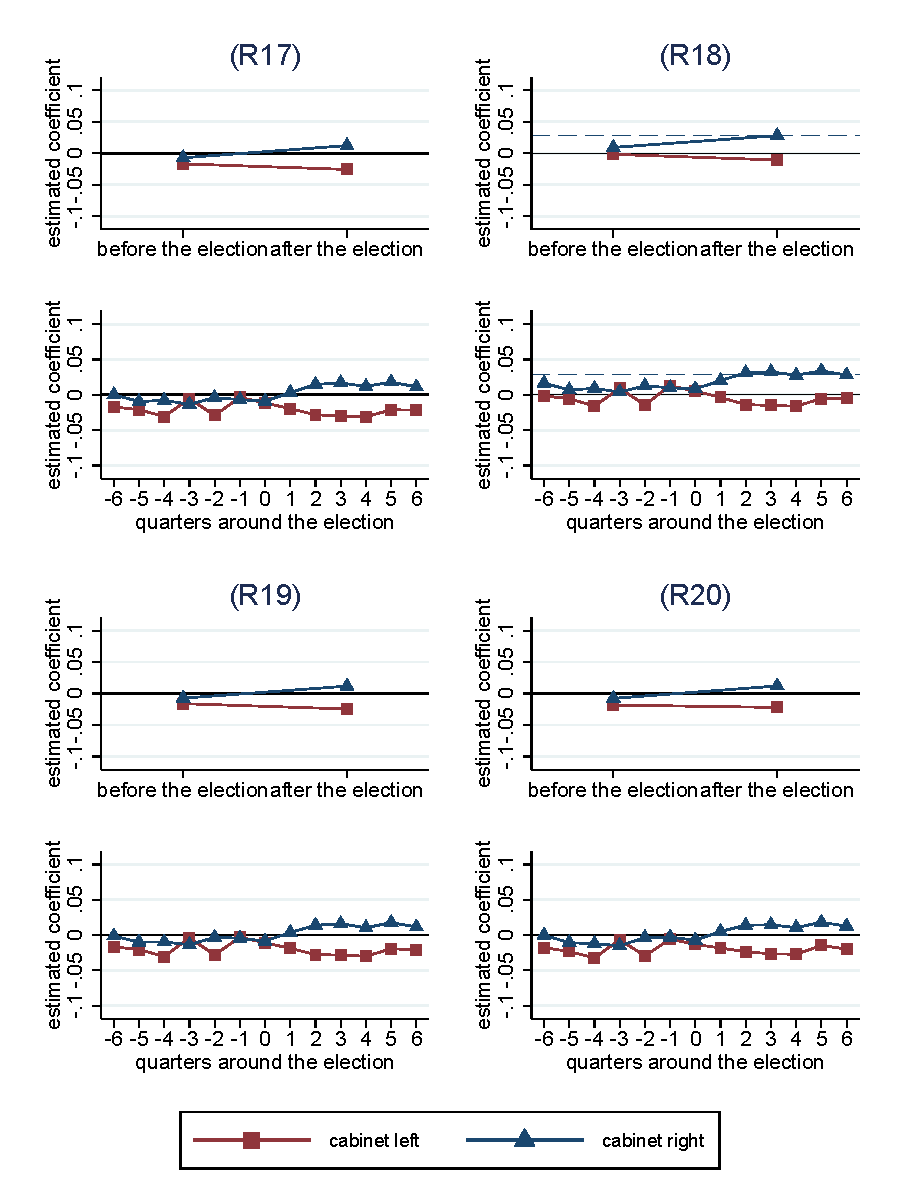
\includegraphics[width=1\textwidth]{../results/decisions/refugeestatus_rate_graphs_R17-R20.pdf}
	\scriptsize{Note: These figures show the time evolution of the share of refugee status decisions in all decisions made in that quarter in fixed effects regression with a set of dummies for before and after the election or a set of dummies for different quarters before and after an election in a quarter t = 0. Significant coefficients are indicated by filled plot markers.}
\end{figure}

\begin{table}[htbp]\centering
\def\sym#1{\ifmmode^{#1}\else\(^{#1}\)\fi}
\caption{Coefficients quarterly model refugeestatus\_rate R17 - R20}
\begin{tabular}{l*{8}{c}}
\hline\hline
                    &\multicolumn{1}{c}{(1)}&\multicolumn{1}{c}{(2)}&\multicolumn{1}{c}{(3)}&\multicolumn{1}{c}{(4)}&\multicolumn{1}{c}{(5)}&\multicolumn{1}{c}{(6)}&\multicolumn{1}{c}{(7)}&\multicolumn{1}{c}{(8)}\\
                    &\multicolumn{1}{c}{left\_R17}&\multicolumn{1}{c}{right\_R17}&\multicolumn{1}{c}{left\_R18}&\multicolumn{1}{c}{right\_R18}&\multicolumn{1}{c}{left\_R19}&\multicolumn{1}{c}{right\_R19}&\multicolumn{1}{c}{left\_R20}&\multicolumn{1}{c}{right\_R20}\\
\hline
 6 quarters before the election&     -0.0172\sym{*}  &  -0.0000339         &    -0.00152         &     -0.0126         &     -0.0166\sym{*}  &    -0.00121         &     -0.0179\sym{*}  &   -0.000107         \\
                    &   (0.00827)         &   (0.00790)         &   (0.00646)         &   (0.00761)         &   (0.00835)         &   (0.00797)         &   (0.00828)         &   (0.00791)         \\
[1em]
 5 quarters before the election&     -0.0210\sym{*}  &    -0.00947         &    -0.00552         &     -0.0222\sym{*}  &     -0.0205\sym{*}  &    -0.00997         &     -0.0231\sym{**} &     -0.0108         \\
                    &   (0.00822)         &   (0.00825)         &   (0.00665)         &   (0.00963)         &   (0.00811)         &   (0.00840)         &   (0.00832)         &   (0.00834)         \\
[1em]
 4 quarters before the election&     -0.0308\sym{**} &    -0.00787         &     -0.0160         &     -0.0201         &     -0.0304\sym{**} &    -0.00973         &     -0.0324\sym{***}&     -0.0122         \\
                    &   (0.00972)         &    (0.0111)         &   (0.00843)         &    (0.0113)         &   (0.00970)         &    (0.0114)         &   (0.00984)         &    (0.0113)         \\
[1em]
 3 quarters before the election&    -0.00539         &     -0.0134         &     0.00918         &     -0.0252\sym{**} &    -0.00384         &     -0.0137         &    -0.00632         &     -0.0150\sym{*}  \\
                    &   (0.00999)         &   (0.00714)         &    (0.0108)         &   (0.00930)         &    (0.0100)         &   (0.00714)         &    (0.0100)         &   (0.00730)         \\
[1em]
 2 quarters before the election&     -0.0291\sym{***}&    -0.00388         &     -0.0142\sym{*}  &     -0.0164\sym{*}  &     -0.0280\sym{***}&    -0.00313         &     -0.0296\sym{***}&    -0.00344         \\
                    &   (0.00753)         &   (0.00985)         &   (0.00679)         &   (0.00816)         &   (0.00746)         &   (0.00976)         &   (0.00764)         &   (0.00986)         \\
[1em]
 1 quarters before the election&    -0.00364         &    -0.00683         &      0.0130         &     -0.0192\sym{*}  &    -0.00311         &    -0.00442         &    -0.00576         &    -0.00283         \\
                    &   (0.00792)         &   (0.00920)         &   (0.00835)         &   (0.00933)         &   (0.00797)         &   (0.00903)         &   (0.00784)         &   (0.00914)         \\
[1em]
Quarter of the election&     -0.0115         &    -0.00909         &     0.00529         &     -0.0208\sym{*}  &     -0.0108         &    -0.00842         &     -0.0131         &    -0.00717         \\
                    &   (0.00725)         &   (0.00742)         &   (0.00903)         &   (0.00912)         &   (0.00721)         &   (0.00749)         &   (0.00725)         &   (0.00695)         \\
[1em]
 1 quarters after the election&     -0.0195\sym{*}  &     0.00312         &    -0.00371         &    -0.00903         &     -0.0189\sym{*}  &     0.00369         &     -0.0183\sym{*}  &     0.00506         \\
                    &   (0.00811)         &   (0.00806)         &    (0.0104)         &   (0.00872)         &   (0.00809)         &   (0.00808)         &   (0.00807)         &   (0.00802)         \\
[1em]
 2 quarters after the election&     -0.0283\sym{***}&      0.0147\sym{*}  &     -0.0139\sym{*}  &     0.00204         &     -0.0276\sym{***}&      0.0140\sym{*}  &     -0.0235\sym{**} &      0.0140\sym{*}  \\
                    &   (0.00714)         &   (0.00707)         &   (0.00653)         &   (0.00753)         &   (0.00713)         &   (0.00702)         &   (0.00748)         &   (0.00705)         \\
[1em]
 3 quarters after the election&     -0.0297\sym{***}&      0.0169\sym{*}  &     -0.0150\sym{*}  &     0.00337         &     -0.0284\sym{***}&      0.0161\sym{*}  &     -0.0266\sym{***}&      0.0146\sym{*}  \\
                    &   (0.00692)         &   (0.00698)         &   (0.00666)         &   (0.00771)         &   (0.00686)         &   (0.00709)         &   (0.00676)         &   (0.00693)         \\
[1em]
 4 quarters after the election&     -0.0312\sym{***}&      0.0118\sym{*}  &     -0.0161\sym{*}  &    -0.00144         &     -0.0299\sym{***}&      0.0104         &     -0.0271\sym{***}&      0.0106         \\
                    &   (0.00833)         &   (0.00597)         &   (0.00641)         &   (0.00800)         &   (0.00814)         &   (0.00618)         &   (0.00793)         &   (0.00599)         \\
[1em]
 5 quarters after the election&     -0.0212\sym{**} &      0.0181         &    -0.00542         &     0.00469         &     -0.0194\sym{**} &      0.0176         &     -0.0146\sym{*}  &      0.0181         \\
                    &   (0.00758)         &   (0.00979)         &   (0.00800)         &   (0.00653)         &   (0.00733)         &   (0.00973)         &   (0.00722)         &   (0.00980)         \\
[1em]
 6 quarters after the election&     -0.0215\sym{*}  &      0.0111         &    -0.00509         &    -0.00109         &     -0.0207\sym{*}  &      0.0116         &     -0.0198\sym{*}  &      0.0127         \\
                    &    (0.0101)         &   (0.00696)         &   (0.00993)         &   (0.00751)         &    (0.0101)         &   (0.00698)         &   (0.00999)         &   (0.00705)         \\
\hline
Observations        &       12921         &       12921         &       12921         &       12921         &       12921         &       12921         &       12868         &       12868         \\
\hline\hline
\multicolumn{9}{l}{\footnotesize Standard errors in parentheses}\\
\multicolumn{9}{l}{\footnotesize \sym{*} \(p<0.05\), \sym{**} \(p<0.01\), \sym{***} \(p<0.001\)}\\
\end{tabular}
\end{table}




% ================================================================================================================================================================
\clearpage
\FloatBarrier
\subsection{Robustness checks for temporary protection decisions}

\begin{table}[htbp]\centering
\def\sym#1{\ifmmode^{#1}\else\(^{#1}\)\fi}
\caption{Determinats of log\_temporary\_protection\_pc}
\begin{tabular}{l*{6}{c}}
\hline\hline
                    &\multicolumn{1}{c}{(1)}&\multicolumn{1}{c}{(2)}&\multicolumn{1}{c}{(3)}&\multicolumn{1}{c}{(4)}&\multicolumn{1}{c}{(5)}&\multicolumn{1}{c}{(6)}\\
                    &\multicolumn{1}{c}{log\_temporary\_protection\_pc}&\multicolumn{1}{c}{log\_temporary\_protection\_pc}&\multicolumn{1}{c}{log\_temporary\_protection\_pc}&\multicolumn{1}{c}{log\_temporary\_protection\_pc}&\multicolumn{1}{c}{log\_temporary\_protection\_pc}&\multicolumn{1}{c}{log\_temporary\_protection\_pc}\\
\hline
Political Terror Scale&      0.0810\sym{*}  &                     &      0.0765\sym{*}  &      0.0820\sym{*}  &      0.0817\sym{*}  &      0.0722         \\
                    &    (0.0340)         &                     &    (0.0336)         &    (0.0347)         &    (0.0345)         &    (0.0377)         \\
[1em]
Civic Liberty (FHI) &      0.0753         &                     &      0.0631         &      0.0813         &      0.0815         &      0.0991         \\
                    &    (0.0674)         &                     &    (0.0591)         &    (0.0660)         &    (0.0660)         &    (0.0747)         \\
[1em]
Political Rights (FHI)&      0.0366         &                     &      0.0272         &      0.0363         &      0.0368         &      0.0360         \\
                    &    (0.0425)         &                     &    (0.0399)         &    (0.0436)         &    (0.0433)         &    (0.0531)         \\
[1em]
Quarterly civil war battle death (000s)&       0.264\sym{***}&                     &       0.223\sym{***}&       0.264\sym{***}&       0.264\sym{***}&       0.259\sym{***}\\
                    &    (0.0251)         &                     &    (0.0223)         &    (0.0249)         &    (0.0248)         &    (0.0233)         \\
[1em]
Log origin country real GDP per capita&      -0.127         &                     &     -0.0630         &      -0.137         &      -0.135         &     -0.0717         \\
                    &    (0.0740)         &                     &    (0.0758)         &    (0.0792)         &    (0.0789)         &     (0.110)         \\
[1em]
Log destination country real GDP per capita&       0.776         &       0.775         &       0.959\sym{*}  &       0.852\sym{*}  &       0.826         &       0.268         \\
                    &     (0.413)         &     (0.435)         &     (0.375)         &     (0.413)         &     (0.415)         &     (0.285)         \\
[1em]
Quarterly unemployment rate at destination&     -0.0199\sym{**} &     -0.0193\sym{**} &    -0.00727         &     -0.0159\sym{*}  &     -0.0183\sym{**} &     -0.0172\sym{**} \\
                    &   (0.00621)         &   (0.00628)         &   (0.00610)         &   (0.00635)         &   (0.00629)         &   (0.00633)         \\
[1em]
Log average past total asylum decisions per capita&                     &                     &      1116.5\sym{***}&                     &                     &                     \\
                    &                     &                     &     (198.3)         &                     &                     &                     \\
[1em]
Log average past dyadic asylum decisions per capita&                     &                     &     13243.6\sym{***}&                     &                     &                     \\
                    &                     &                     &    (2142.8)         &                     &                     &                     \\
[1em]
after 2007          &                     &                     &                     &                     &      0.0809         &                     \\
                    &                     &                     &                     &                     &     (0.115)         &                     \\
[1em]
Weighted cabinet position right&      -0.190\sym{***}&      -0.187\sym{***}&      -0.225\sym{***}&                     &      -0.185\sym{***}&      -0.232\sym{***}\\
                    &    (0.0458)         &    (0.0449)         &    (0.0450)         &                     &    (0.0440)         &    (0.0431)         \\
[1em]
Cabinet position left * Before the election&      0.0549         &      0.0442         &      0.0484         &       0.156\sym{***}&      0.0571\sym{*}  &     -0.0387         \\
                    &    (0.0287)         &    (0.0280)         &    (0.0276)         &    (0.0232)         &    (0.0281)         &    (0.0275)         \\
[1em]
Cabinet position left * After the election&      0.0558\sym{*}  &      0.0567\sym{*}  &      0.0352         &       0.153\sym{***}&      0.0547\sym{*}  &      0.0111         \\
                    &    (0.0231)         &    (0.0226)         &    (0.0213)         &    (0.0208)         &    (0.0230)         &    (0.0200)         \\
[1em]
Cabinet position right * Before the election&      0.0500         &      0.0521\sym{*}  &      0.0559\sym{*}  &     -0.0317         &      0.0485         &      0.0384\sym{*}  \\
                    &    (0.0252)         &    (0.0247)         &    (0.0238)         &    (0.0227)         &    (0.0251)         &    (0.0177)         \\
[1em]
Cabinet position right * After the election&       0.157\sym{***}&       0.156\sym{***}&       0.186\sym{***}&      0.0772\sym{*}  &       0.159\sym{***}&       0.109\sym{***}\\
                    &    (0.0316)         &    (0.0320)         &    (0.0321)         &    (0.0305)         &    (0.0319)         &    (0.0238)         \\
\hline
Observations        &       15938         &       15938         &       15938         &       15938         &       15938         &       21953         \\
Adjusted \(R^{2}\)  &       0.527         &       0.541         &       0.133         &       0.086         &       0.088         &       0.093         \\
Fixed Effects       &           O         &       O x T         &       D x O         &       D x O         &       D x O         &       D x O         \\
Destination dummies &         Yes         &         Yes         &          No         &          No         &          No         &          No         \\
Quarter-Year dummies&         Yes         &          No         &         Yes         &         Yes         &         Yes         &         Yes         \\
\hline\hline
\multicolumn{7}{l}{\footnotesize Standard errors in parentheses}\\
\multicolumn{7}{l}{\footnotesize \sym{*} \(p<0.05\), \sym{**} \(p<0.01\), \sym{***} \(p<0.001\)}\\
\end{tabular}
\end{table}


\clearpage
\FloatBarrier
\begin{figure}[!ht]
	\caption{Temporary protection decisions per capita: predicted pattern - R1 to R6}
	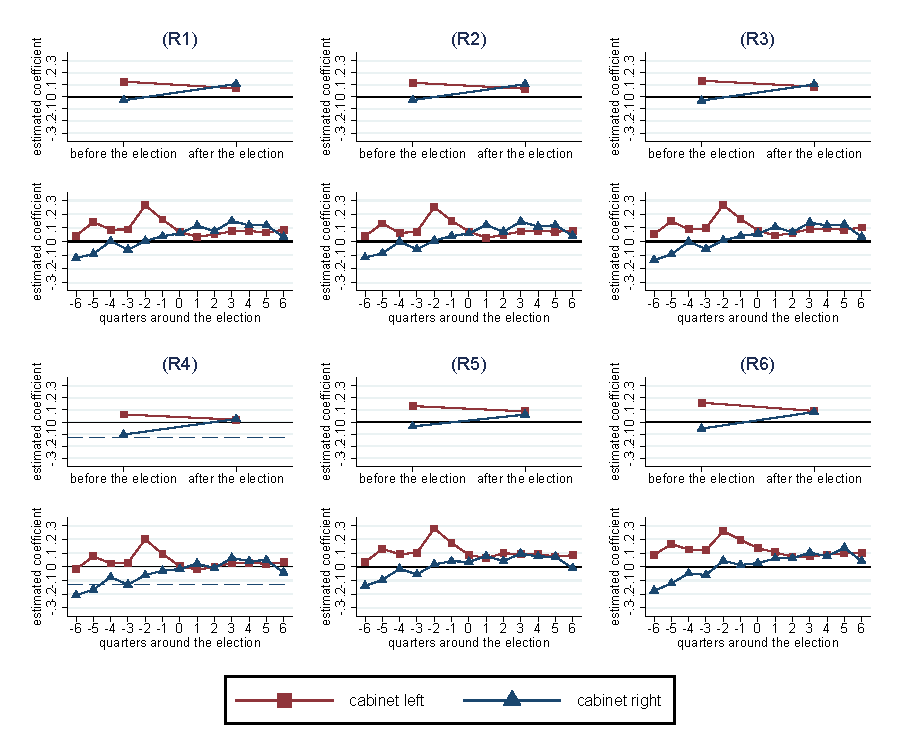
\includegraphics[width=1\textwidth]{../results/decisions/log_temporary_protection_pc_graphs_R1-R6.pdf}
	\scriptsize{Note: These figures show the time evolution of temporary protection decisions decisions as estimated in fixed effects regression with a set of dummies for before and after the election or a set of dummies for different quarters before and after an election in a quarter t = 0. Significant coefficients are indicated by filled plot markers.}
\end{figure}

\clearpage
\FloatBarrier

\begin{table}[htbp]\centering
\def\sym#1{\ifmmode^{#1}\else\(^{#1}\)\fi}
\caption{Coefficients quarterly model log\_temporary\_protection\_pc R1 - R3}
\begin{tabular}{l*{6}{c}}
\hline\hline
                    &\multicolumn{1}{c}{(1)}&\multicolumn{1}{c}{(2)}&\multicolumn{1}{c}{(3)}&\multicolumn{1}{c}{(4)}&\multicolumn{1}{c}{(5)}&\multicolumn{1}{c}{(6)}\\
                    &\multicolumn{1}{c}{left\_R1}&\multicolumn{1}{c}{right\_R1}&\multicolumn{1}{c}{left\_R2}&\multicolumn{1}{c}{right\_R2}&\multicolumn{1}{c}{left\_R3}&\multicolumn{1}{c}{right\_R3}\\
\hline
 6 quarters before the election&      0.0428         &      -0.121\sym{***}&      0.0392         &      -0.116\sym{***}&      0.0534         &      -0.135\sym{***}\\
                    &    (0.0351)         &    (0.0299)         &    (0.0357)         &    (0.0295)         &    (0.0337)         &    (0.0306)         \\
[1em]
 5 quarters before the election&       0.142\sym{***}&     -0.0903\sym{**} &       0.132\sym{**} &     -0.0866\sym{**} &       0.148\sym{***}&     -0.0938\sym{**} \\
                    &    (0.0403)         &    (0.0292)         &    (0.0427)         &    (0.0306)         &    (0.0412)         &    (0.0290)         \\
[1em]
 4 quarters before the election&      0.0874\sym{*}  &     0.00286         &      0.0628         &    -0.00127         &      0.0896\sym{*}  &   -0.000661         \\
                    &    (0.0429)         &    (0.0355)         &    (0.0424)         &    (0.0353)         &    (0.0431)         &    (0.0348)         \\
[1em]
 3 quarters before the election&      0.0883\sym{*}  &     -0.0602         &      0.0718         &     -0.0566         &      0.0962\sym{*}  &     -0.0545         \\
                    &    (0.0408)         &    (0.0364)         &    (0.0418)         &    (0.0383)         &    (0.0405)         &    (0.0347)         \\
[1em]
 2 quarters before the election&       0.264\sym{***}&     0.00536         &       0.252\sym{***}&     0.00722         &       0.267\sym{***}&     0.00841         \\
                    &    (0.0364)         &    (0.0472)         &    (0.0390)         &    (0.0478)         &    (0.0360)         &    (0.0458)         \\
[1em]
 1 quarters before the election&       0.162\sym{***}&      0.0382         &       0.153\sym{***}&      0.0399         &       0.166\sym{***}&      0.0403         \\
                    &    (0.0412)         &    (0.0464)         &    (0.0415)         &    (0.0477)         &    (0.0408)         &    (0.0457)         \\
[1em]
Quarter of the election&      0.0685\sym{*}  &      0.0605         &      0.0734\sym{*}  &      0.0589         &      0.0807\sym{*}  &      0.0580         \\
                    &    (0.0328)         &    (0.0427)         &    (0.0326)         &    (0.0438)         &    (0.0326)         &    (0.0430)         \\
[1em]
 1 quarters after the election&      0.0359         &       0.117\sym{*}  &      0.0272         &       0.121\sym{*}  &      0.0441         &       0.107\sym{*}  \\
                    &    (0.0342)         &    (0.0478)         &    (0.0342)         &    (0.0490)         &    (0.0341)         &    (0.0451)         \\
[1em]
 2 quarters after the election&      0.0512         &      0.0757         &      0.0499         &      0.0717         &      0.0619\sym{*}  &      0.0682         \\
                    &    (0.0328)         &    (0.0463)         &    (0.0327)         &    (0.0475)         &    (0.0312)         &    (0.0445)         \\
[1em]
 3 quarters after the election&      0.0749\sym{*}  &       0.150\sym{***}&      0.0734\sym{*}  &       0.146\sym{***}&      0.0916\sym{**} &       0.139\sym{**} \\
                    &    (0.0315)         &    (0.0439)         &    (0.0330)         &    (0.0439)         &    (0.0290)         &    (0.0426)         \\
[1em]
 4 quarters after the election&      0.0778\sym{**} &       0.118\sym{**} &      0.0787\sym{**} &       0.110\sym{*}  &      0.0960\sym{**} &       0.117\sym{**} \\
                    &    (0.0293)         &    (0.0424)         &    (0.0296)         &    (0.0444)         &    (0.0293)         &    (0.0408)         \\
[1em]
 5 quarters after the election&      0.0660         &       0.119\sym{**} &      0.0722\sym{*}  &       0.120\sym{**} &      0.0856\sym{*}  &       0.124\sym{**} \\
                    &    (0.0355)         &    (0.0428)         &    (0.0357)         &    (0.0434)         &    (0.0347)         &    (0.0411)         \\
[1em]
 6 quarters after the election&      0.0857\sym{**} &      0.0338         &      0.0784\sym{*}  &      0.0423         &       0.103\sym{***}&      0.0344         \\
                    &    (0.0327)         &    (0.0355)         &    (0.0338)         &    (0.0352)         &    (0.0306)         &    (0.0341)         \\
\hline
Observations        &       15938         &       15938         &       15938         &       15938         &       15938         &       15938         \\
\hline\hline
\multicolumn{7}{l}{\footnotesize Standard errors in parentheses}\\
\multicolumn{7}{l}{\footnotesize \sym{*} \(p<0.05\), \sym{**} \(p<0.01\), \sym{***} \(p<0.001\)}\\
\end{tabular}
\end{table}

\begin{table}[htbp]\centering
\def\sym#1{\ifmmode^{#1}\else\(^{#1}\)\fi}
\caption{Coefficients log\_temporary\_protection\_pc R4 - R6}
\begin{tabular}{l*{6}{c}}
\hline\hline
                    &\multicolumn{1}{c}{(1)}&\multicolumn{1}{c}{(2)}&\multicolumn{1}{c}{(3)}&\multicolumn{1}{c}{(4)}&\multicolumn{1}{c}{(5)}&\multicolumn{1}{c}{(6)}\\
                    &\multicolumn{1}{c}{left\_R4}&\multicolumn{1}{c}{right\_R4}&\multicolumn{1}{c}{left\_R5}&\multicolumn{1}{c}{right\_R5}&\multicolumn{1}{c}{left\_R6}&\multicolumn{1}{c}{right\_R6}\\
\hline
 6 quarters before the election&      0.0837\sym{*}  &      -0.176\sym{***}&     -0.0135         &     -0.0937\sym{**} &     -0.0490         &     -0.0919\sym{***}\\
                    &    (0.0344)         &    (0.0344)         &    (0.0371)         &    (0.0301)         &    (0.0316)         &    (0.0209)         \\
[1em]
 5 quarters before the election&       0.161\sym{***}&      -0.108\sym{***}&      0.0627         &     -0.0254         &     -0.0274         &     -0.0163         \\
                    &    (0.0463)         &    (0.0322)         &    (0.0415)         &    (0.0340)         &    (0.0362)         &    (0.0246)         \\
[1em]
 4 quarters before the election&       0.105\sym{*}  &     -0.0152         &      0.0105         &      0.0652         &     -0.0863\sym{*}  &      0.0429         \\
                    &    (0.0450)         &    (0.0353)         &    (0.0467)         &    (0.0354)         &    (0.0422)         &    (0.0307)         \\
[1em]
 3 quarters before the election&       0.118\sym{**} &     -0.0378         &      0.0249         &      0.0383         &     -0.0761         &      0.0159         \\
                    &    (0.0417)         &    (0.0334)         &    (0.0476)         &    (0.0342)         &    (0.0427)         &    (0.0253)         \\
[1em]
 2 quarters before the election&       0.285\sym{***}&      0.0390         &       0.191\sym{***}&       0.118\sym{*}  &      0.0313         &      0.0732\sym{*}  \\
                    &    (0.0375)         &    (0.0456)         &    (0.0424)         &    (0.0477)         &    (0.0355)         &    (0.0363)         \\
[1em]
 1 quarters before the election&       0.182\sym{***}&      0.0670         &      0.0790         &       0.148\sym{**} &     -0.0279         &       0.148\sym{***}\\
                    &    (0.0416)         &    (0.0494)         &    (0.0472)         &    (0.0519)         &    (0.0404)         &    (0.0340)         \\
[1em]
Quarter of the election&       0.117\sym{***}&      0.0718         &      0.0121         &       0.146\sym{**} &     -0.0622         &       0.121\sym{***}\\
                    &    (0.0340)         &    (0.0471)         &    (0.0399)         &    (0.0518)         &    (0.0338)         &    (0.0356)         \\
[1em]
 1 quarters after the election&       0.100\sym{**} &      0.0532         &   -0.000135         &       0.131\sym{**} &     -0.0489         &      0.0699\sym{*}  \\
                    &    (0.0339)         &    (0.0453)         &    (0.0400)         &    (0.0459)         &    (0.0299)         &    (0.0307)         \\
[1em]
 2 quarters after the election&       0.105\sym{***}&      0.0361         &      0.0125         &       0.114\sym{*}  &     -0.0373         &      0.0673\sym{*}  \\
                    &    (0.0319)         &    (0.0463)         &    (0.0418)         &    (0.0497)         &    (0.0362)         &    (0.0313)         \\
[1em]
 3 quarters after the election&       0.160\sym{***}&      0.0937\sym{*}  &      0.0670\sym{*}  &       0.178\sym{***}&    -0.00420         &       0.150\sym{***}\\
                    &    (0.0294)         &    (0.0451)         &    (0.0302)         &    (0.0451)         &    (0.0293)         &    (0.0389)         \\
[1em]
 4 quarters after the election&       0.167\sym{***}&       0.100\sym{*}  &      0.0702\sym{*}  &       0.183\sym{***}&     0.00717         &       0.102\sym{***}\\
                    &    (0.0326)         &    (0.0415)         &    (0.0336)         &    (0.0399)         &    (0.0271)         &    (0.0286)         \\
[1em]
 5 quarters after the election&       0.180\sym{***}&       0.123\sym{**} &      0.0798\sym{*}  &       0.206\sym{***}&      0.0915\sym{**} &       0.172\sym{***}\\
                    &    (0.0398)         &    (0.0395)         &    (0.0368)         &    (0.0404)         &    (0.0307)         &    (0.0324)         \\
[1em]
 6 quarters after the election&       0.179\sym{***}&      0.0301         &      0.0729\sym{**} &       0.108\sym{**} &      0.0585\sym{*}  &      0.0906\sym{***}\\
                    &    (0.0338)         &    (0.0328)         &    (0.0262)         &    (0.0338)         &    (0.0228)         &    (0.0265)         \\
\hline
Observations        &       15938         &       15938         &       15938         &       15938         &       21953         &       21953         \\
\hline\hline
\multicolumn{7}{l}{\footnotesize Standard errors in parentheses}\\
\multicolumn{7}{l}{\footnotesize \sym{*} \(p<0.05\), \sym{**} \(p<0.01\), \sym{***} \(p<0.001\)}\\
\end{tabular}
\end{table}




\clearpage
\FloatBarrier
\begin{table}[htbp]\centering \scriptsize
\def\sym#1{\ifmmode^{#1}\else\(^{#1}\)\fi}
\caption{Determinats of log\_temporary\_protection\_pc - R7 - R10}
\begin{tabular}{l*{4}{c}}
\hline\hline
                    &\multicolumn{1}{c}{(R7)}&\multicolumn{1}{c}{(R8)}&\multicolumn{1}{c}{(R9)}&\multicolumn{1}{c}{(R10)}\\
\hline
Political Terror Scale&      0.0777\sym{*}  &                     &     0.00485         &     0.00485         \\
                    &    (0.0357)         &                     &    (0.0409)         &    (0.0409)         \\
[0,5em]
Civic Liberty (FHI) &      0.0736         &                     &      0.0758         &      0.0758         \\
                    &    (0.0650)         &                     &    (0.0628)         &    (0.0628)         \\
[0,5em]
Political Rights (FHI)&      0.0322         &                     &      0.0271         &      0.0271         \\
                    &    (0.0433)         &                     &    (0.0502)         &    (0.0502)         \\
[0,5em]
Quarterly civil war&       0.270\sym{***}&                     &       0.219\sym{***}&       0.219\sym{***}\\
 battle death (000s)                    &    (0.0248)         &                     &    (0.0201)         &    (0.0201)         \\
[0,5em]
Log origin country&      -0.110         &                     &      0.0346         &      0.0346         \\
 real GDP per capita                    &    (0.0789)         &                     &     (0.100)         &     (0.100)         \\
[0,5em]
Log destination country&       1.553\sym{***}&       1.307\sym{***}&       0.455         &       0.455         \\
 quarterly real GDP per capita                    &     (0.379)         &     (0.328)         &     (0.266)         &     (0.266)         \\
[0,5em]
Quarterly unemployment&      0.0127         &     0.00230         &     -0.0129\sym{*}  &     -0.0129\sym{*}  \\
  rate at destination                   &   (0.00656)         &   (0.00561)         &   (0.00521)         &   (0.00521)         \\
[0,5em]
Log total dyadic decisions&                     &       0.277\sym{***}&       0.234\sym{***}&       0.234\sym{***}\\
per capita                    &                     &    (0.0424)         &    (0.0312)         &    (0.0312)         \\
[0,5em]
Log total decisions at &       0.314\sym{***}&      0.0898\sym{**} &                     &                     \\
 destination per capita                    &    (0.0429)         &    (0.0277)         &                     &                     \\
[0,5em]
Years after 2007    &                     &                     &                     &       0.130         \\
                    &                     &                     &                     &     (0.125)         \\
[0,5em]
Cabinet position left *&       0.121\sym{***}&       0.124\sym{***}&      0.0847\sym{***}&      0.0847\sym{***}\\
 Before the election                    &    (0.0223)         &    (0.0204)         &    (0.0176)         &    (0.0176)         \\
[0,5em]
Cabinet position left *n&       0.107\sym{***}&      0.0741\sym{***}&      0.0886\sym{***}&      0.0886\sym{***}\\
 After the electio                    &    (0.0182)         &    (0.0186)         &    (0.0162)         &    (0.0162)         \\
[0,5em]
Cabinet position right *&     -0.0366         &     -0.0339         &     -0.0646\sym{**} &     -0.0646\sym{**} \\
 Before the election                    &    (0.0233)         &    (0.0209)         &    (0.0187)         &    (0.0187)         \\
[0,5em]
Cabinet position right * &      0.0861\sym{**} &       0.102\sym{**} &      0.0356         &      0.0356         \\
 After the election                   &    (0.0312)         &    (0.0325)         &    (0.0202)         &    (0.0202)         \\
\hline
Observations        &       15938         &       15938         &       21952         &       21952         \\
Adjusted \(R^{2}\)  &       0.111         &       0.146         &       0.177         &       0.177         \\
Fixed Effects       &       D x O         &       D x O         &       D x O         &       D x O         \\
Destination dummies &          No         &          No         &          No         &          No         \\
Quarter-Year dummies&         Yes         &         Yes         &         Yes         &         Yes         \\
\hline\hline
\multicolumn{5}{l}{ Standard errors in parentheses \sym{*} \(p<0.05\), \sym{**} \(p<0.01\), \sym{***} \(p<0.001\)}\\
\end{tabular}
\end{table}


\clearpage
\FloatBarrier
\begin{figure}[!ht]
	\caption{Temporary protection decisions per capita: predicted pattern - R7 to R10}
	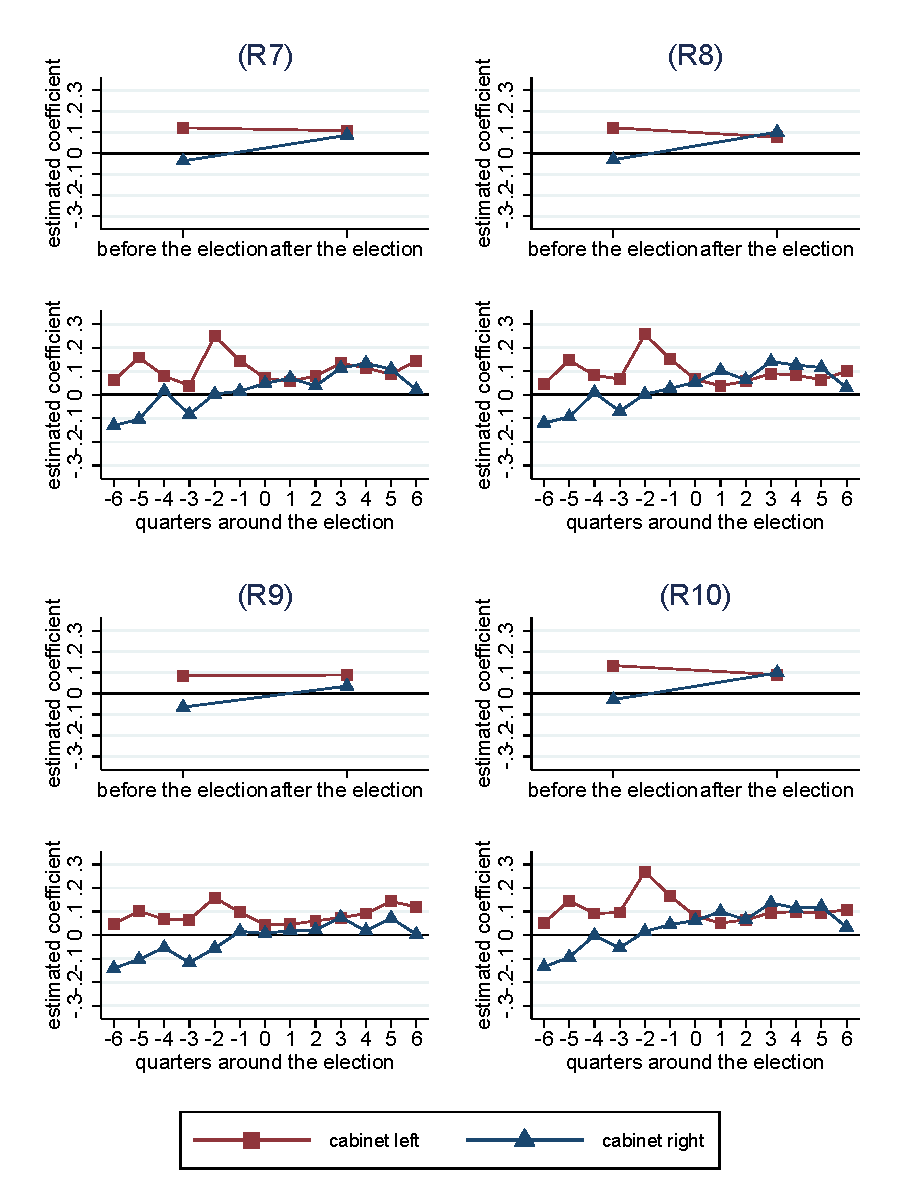
\includegraphics[width=1\textwidth]{../results/decisions/log_temporary_protection_pc_graphs_R7-R10.pdf}
	\scriptsize{Note: These figures show the time evolution of temporary protection decisions as estimated in fixed effects regression with a set of dummies for before and after the election or a set of dummies for different quarters before and after an election in a quarter t = 0. Significant coefficients are indicated by filled plot markers.}
\end{figure}

\begin{table}[htbp]\centering
\def\sym#1{\ifmmode^{#1}\else\(^{#1}\)\fi}
\caption{Coefficients quarterly model log\_temporary\_protection\_pc R7 - R10}
\begin{tabular}{l*{8}{c}}
\hline\hline
                    &\multicolumn{1}{c}{(1)}&\multicolumn{1}{c}{(2)}&\multicolumn{1}{c}{(3)}&\multicolumn{1}{c}{(4)}&\multicolumn{1}{c}{(5)}&\multicolumn{1}{c}{(6)}&\multicolumn{1}{c}{(7)}&\multicolumn{1}{c}{(8)}\\
                    &\multicolumn{1}{c}{left\_R7}&\multicolumn{1}{c}{right\_R7}&\multicolumn{1}{c}{left\_R8}&\multicolumn{1}{c}{right\_R8}&\multicolumn{1}{c}{left\_R9}&\multicolumn{1}{c}{right\_R9}&\multicolumn{1}{c}{left\_R10}&\multicolumn{1}{c}{right\_R10}\\
\hline
 6 quarters before the election&      0.0610         &      -0.130\sym{***}&      0.0454         &      -0.120\sym{***}&      0.0488         &      -0.141\sym{***}&      0.0519         &      -0.135\sym{***}\\
                    &    (0.0348)         &    (0.0346)         &    (0.0336)         &    (0.0318)         &    (0.0270)         &    (0.0260)         &    (0.0336)         &    (0.0306)         \\
[1em]
 5 quarters before the election&       0.159\sym{***}&      -0.104\sym{**} &       0.147\sym{***}&     -0.0936\sym{**} &       0.102\sym{**} &      -0.103\sym{***}&       0.146\sym{***}&     -0.0941\sym{**} \\
                    &    (0.0465)         &    (0.0326)         &    (0.0413)         &    (0.0291)         &    (0.0327)         &    (0.0233)         &    (0.0409)         &    (0.0288)         \\
[1em]
 4 quarters before the election&      0.0795         &      0.0162         &      0.0829         &     0.00962         &      0.0663\sym{*}  &     -0.0532         &      0.0917\sym{*}  &    -0.00152         \\
                    &    (0.0449)         &    (0.0357)         &    (0.0430)         &    (0.0352)         &    (0.0321)         &    (0.0335)         &    (0.0432)         &    (0.0349)         \\
[1em]
 3 quarters before the election&      0.0394         &     -0.0827\sym{*}  &      0.0672         &     -0.0700\sym{*}  &      0.0657\sym{*}  &      -0.117\sym{***}&      0.0961\sym{*}  &     -0.0539         \\
                    &    (0.0403)         &    (0.0348)         &    (0.0381)         &    (0.0340)         &    (0.0325)         &    (0.0315)         &    (0.0403)         &    (0.0348)         \\
[1em]
 2 quarters before the election&       0.249\sym{***}&     0.00308         &       0.257\sym{***}&     0.00253         &       0.159\sym{***}&     -0.0555         &       0.269\sym{***}&      0.0147         \\
                    &    (0.0369)         &    (0.0462)         &    (0.0351)         &    (0.0457)         &    (0.0272)         &    (0.0369)         &    (0.0359)         &    (0.0459)         \\
[1em]
 1 quarters before the election&       0.145\sym{***}&      0.0159         &       0.153\sym{***}&      0.0268         &      0.0966\sym{**} &      0.0157         &       0.166\sym{***}&      0.0449         \\
                    &    (0.0409)         &    (0.0474)         &    (0.0404)         &    (0.0450)         &    (0.0319)         &    (0.0306)         &    (0.0407)         &    (0.0464)         \\
[1em]
Quarter of the election&      0.0708\sym{*}  &      0.0481         &      0.0652\sym{*}  &      0.0534         &      0.0438         &     0.00691         &      0.0803\sym{*}  &      0.0618         \\
                    &    (0.0333)         &    (0.0474)         &    (0.0321)         &    (0.0429)         &    (0.0269)         &    (0.0270)         &    (0.0327)         &    (0.0429)         \\
[1em]
 1 quarters after the election&      0.0564         &      0.0712         &      0.0382         &       0.103\sym{*}  &      0.0452         &      0.0195         &      0.0516         &      0.0997\sym{*}  \\
                    &    (0.0349)         &    (0.0454)         &    (0.0342)         &    (0.0464)         &    (0.0243)         &    (0.0313)         &    (0.0338)         &    (0.0465)         \\
[1em]
 2 quarters after the election&      0.0807\sym{**} &      0.0379         &      0.0578         &      0.0637         &      0.0603\sym{*}  &      0.0216         &      0.0644\sym{*}  &      0.0651         \\
                    &    (0.0313)         &    (0.0463)         &    (0.0313)         &    (0.0456)         &    (0.0258)         &    (0.0276)         &    (0.0316)         &    (0.0455)         \\
[1em]
 3 quarters after the election&       0.134\sym{***}&       0.114\sym{*}  &      0.0900\sym{**} &       0.141\sym{**} &      0.0742\sym{**} &      0.0744\sym{*}  &      0.0953\sym{**} &       0.137\sym{**} \\
                    &    (0.0282)         &    (0.0451)         &    (0.0291)         &    (0.0431)         &    (0.0256)         &    (0.0332)         &    (0.0295)         &    (0.0432)         \\
[1em]
 4 quarters after the election&       0.114\sym{***}&       0.134\sym{**} &      0.0836\sym{**} &       0.126\sym{**} &      0.0916\sym{***}&      0.0184         &      0.0993\sym{***}&       0.114\sym{**} \\
                    &    (0.0299)         &    (0.0428)         &    (0.0289)         &    (0.0421)         &    (0.0242)         &    (0.0266)         &    (0.0297)         &    (0.0415)         \\
[1em]
 5 quarters after the election&      0.0874\sym{*}  &       0.109\sym{**} &      0.0639         &       0.115\sym{**} &       0.143\sym{***}&      0.0723\sym{*}  &      0.0936\sym{**} &       0.121\sym{**} \\
                    &    (0.0365)         &    (0.0402)         &    (0.0356)         &    (0.0417)         &    (0.0321)         &    (0.0283)         &    (0.0348)         &    (0.0414)         \\
[1em]
 6 quarters after the election&       0.145\sym{***}&      0.0211         &       0.100\sym{**} &      0.0299         &       0.120\sym{***}&     0.00286         &       0.108\sym{***}&      0.0336         \\
                    &    (0.0320)         &    (0.0336)         &    (0.0306)         &    (0.0343)         &    (0.0241)         &    (0.0248)         &    (0.0310)         &    (0.0342)         \\
\hline
Observations        &       15938         &       15938         &       15938         &       15938         &       21952         &       21952         &       15938         &       15938         \\
\hline\hline
\multicolumn{9}{l}{\footnotesize Standard errors in parentheses}\\
\multicolumn{9}{l}{\footnotesize \sym{*} \(p<0.05\), \sym{**} \(p<0.01\), \sym{***} \(p<0.001\)}\\
\end{tabular}
\end{table}



\clearpage
\FloatBarrier
\begin{table}[htbp]\centering \scriptsize
\def\sym#1{\ifmmode^{#1}\else\(^{#1}\)\fi}
\caption{Determinats of log\_temporary\_protection\_pc - R11 - R16}
\begin{tabular}{l*{6}{c}}
\hline\hline
                    &\multicolumn{1}{c}{(R11)}&\multicolumn{1}{c}{(R12)}&\multicolumn{1}{c}{(R13)}&\multicolumn{1}{c}{(R14)}&\multicolumn{1}{c}{(R15)}&\multicolumn{1}{c}{(R16)}\\
\hline
Political Terror Scale&      0.0770\sym{*}  &   -0.000959         &     0.00340         &      0.0815\sym{*}  &      0.0235         &      0.0274         \\
                    &    (0.0357)         &    (0.0343)         &    (0.0339)         &    (0.0355)         &    (0.0353)         &    (0.0350)         \\
[0,5em]
Civic Liberty (FHI) &      0.0740         &      0.0466         &      0.0468         &      0.0745         &      0.0599         &      0.0591         \\
                    &    (0.0652)         &    (0.0583)         &    (0.0579)         &    (0.0661)         &    (0.0561)         &    (0.0566)         \\
[0,5em]
Political Rights (FHI)&      0.0326         &      0.0273         &      0.0268         &      0.0319         &      0.0227         &      0.0227         \\
                    &    (0.0434)         &    (0.0428)         &    (0.0427)         &    (0.0432)         &    (0.0431)         &    (0.0430)         \\
[0,5em]
Quarterly civil war&       0.270\sym{***}&       0.224\sym{***}&       0.228\sym{***}&       0.269\sym{***}&       0.236\sym{***}&       0.240\sym{***}\\
 battle death (000s)                    &    (0.0249)         &    (0.0199)         &    (0.0215)         &    (0.0248)         &    (0.0242)         &    (0.0254)         \\
[0,5em]
Log origin country&      -0.112         &     0.00748         &     0.00480         &      -0.115         &     -0.0385         &     -0.0382         \\
 real GDP per capita                    &    (0.0791)         &    (0.0645)         &    (0.0649)         &    (0.0803)         &    (0.0702)         &    (0.0710)         \\
[0,5em]
Log destination country&       1.456\sym{***}&       0.949\sym{*}  &       1.127\sym{**} &       1.266\sym{**} &       1.002\sym{*}  &       1.164\sym{**} \\
 quarterly real GDP per capita                    &     (0.383)         &     (0.388)         &     (0.361)         &     (0.388)         &     (0.401)         &     (0.370)         \\
[0,5em]
Quarterly unemployment&     0.00963         &    -0.00966         &    -0.00230         &     0.00184         &    -0.00725         &    -0.00116         \\
 rate at destination                    &   (0.00664)         &   (0.00581)         &   (0.00552)         &   (0.00624)         &   (0.00623)         &   (0.00589)         \\
[0,5em]
Log total decisions at destination&       0.313\sym{***}&                     &      0.0955\sym{*}  &                     &                     &                      \\
 per capita in previous year                   &    (0.0451)         &                     &    (0.0390)         &                     &                     &                     \\
[0,5em]
Log dyadic decisions at destination&                     &       0.284\sym{***}&       0.263\sym{***}&                     &                     &                     \\
  per capita in previous year                   &                     &    (0.0357)         &    (0.0363)         &                     &                     &                     \\
[0,5em]
Log total first-time applications&                     &                     &                     &       0.188\sym{***}&                     &      0.0725\sym{*}  \\
 in the previous 2 quarters                    &                     &                     &                     &    (0.0375)         &                     &    (0.0352)         \\
[0,5em]
Log dyadic first-time applications&                     &                     &                     &                     &       0.146\sym{***}&       0.135\sym{***}\\
  in the previous 2 quarters                   &                     &                     &                     &                     &    (0.0204)         &    (0.0205)         \\
[0,5em]
Cabinet position left *&       0.133\sym{***}&       0.146\sym{***}&       0.139\sym{***}&       0.150\sym{***}&       0.147\sym{***}&       0.146\sym{***}\\
  Before the election                   &    (0.0228)         &    (0.0231)         &    (0.0225)         &    (0.0232)         &    (0.0238)         &    (0.0238)         \\
[0,5em]
Cabinet position left * &       0.111\sym{***}&      0.0915\sym{***}&      0.0829\sym{***}&       0.134\sym{***}&       0.119\sym{***}&       0.114\sym{***}\\
  After the election                  &    (0.0185)         &    (0.0185)         &    (0.0179)         &    (0.0199)         &    (0.0202)         &    (0.0196)         \\
[0,5em]
Cabinet position right *&     -0.0309         &     -0.0268         &     -0.0270         &     -0.0322         &     -0.0379         &     -0.0380         \\
  Before the election                   &    (0.0233)         &    (0.0221)         &    (0.0223)         &    (0.0231)         &    (0.0232)         &    (0.0233)         \\
[0,5em]
Cabinet position right * &      0.0918\sym{**} &       0.110\sym{**} &       0.112\sym{***}&      0.0881\sym{**} &      0.0872\sym{**} &      0.0902\sym{**} \\
 After the election                   &    (0.0312)         &    (0.0318)         &    (0.0318)         &    (0.0309)         &    (0.0320)         &    (0.0318)         \\
\hline
Observations        &       15938         &       15938         &       15938         &       15906         &       15882         &       15882         \\
Adjusted \(R^{2}\)  &       0.108         &       0.156         &       0.158         &       0.095         &       0.115         &       0.116         \\
Fixed Effects       &       D x O         &       D x O         &       D x O         &       D x O         &       D x O         &       D x O         \\
Destination dummies &          No         &          No         &          No         &          No         &          No         &          No         \\
Quarter-Year dummies&         Yes         &         Yes         &         Yes         &         Yes         &         Yes         &         Yes         \\
\hline\hline
\multicolumn{7}{l}{Standard errors in parentheses \sym{*} \(p<0.05\), \sym{**} \(p<0.01\), \sym{***} \(p<0.001\)}\\
\end{tabular}
\end{table}


\clearpage
\FloatBarrier
\begin{figure}[!ht]
	\caption{Temporary protection decisions per capita: predicted pattern - R11 to R16}
	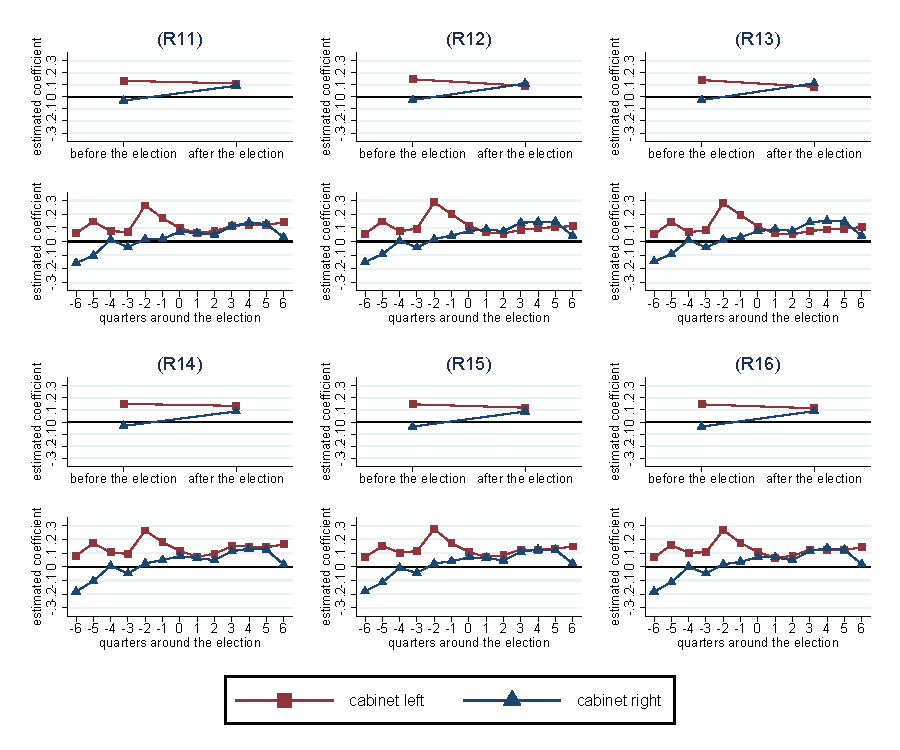
\includegraphics[width=1\textwidth]{../results/decisions/log_temporary_protection_pc_graphs_R11-R16.pdf}
	\scriptsize{Note: These figures show the time evolution of temporary protection decisions as estimated in fixed effects regression with a set of dummies for before and after the election or a set of dummies for different quarters before and after an election in a quarter t = 0. Significant coefficients are indicated by filled plot markers.}
\end{figure}

\clearpage
\FloatBarrier
\begin{table}[htbp]\centering
\def\sym#1{\ifmmode^{#1}\else\(^{#1}\)\fi}
\caption{Coefficients quarterly model log\_temporary\_protection\_pc R11 - R13}
\begin{tabular}{l*{6}{c}}
\hline\hline
                    &\multicolumn{1}{c}{(1)}&\multicolumn{1}{c}{(2)}&\multicolumn{1}{c}{(3)}&\multicolumn{1}{c}{(4)}&\multicolumn{1}{c}{(5)}&\multicolumn{1}{c}{(6)}\\
                    &\multicolumn{1}{c}{left\_R11}&\multicolumn{1}{c}{right\_R11}&\multicolumn{1}{c}{left\_R12}&\multicolumn{1}{c}{right\_R12}&\multicolumn{1}{c}{left\_R13}&\multicolumn{1}{c}{right\_R13}\\
\hline
 6 quarters before the election&      0.0615         &      -0.156\sym{***}&      0.0580         &      -0.150\sym{***}&      0.0531         &      -0.146\sym{***}\\
                    &    (0.0344)         &    (0.0342)         &    (0.0357)         &    (0.0326)         &    (0.0354)         &    (0.0331)         \\
[1em]
 5 quarters before the election&       0.147\sym{**} &      -0.103\sym{**} &       0.147\sym{***}&     -0.0921\sym{**} &       0.144\sym{***}&     -0.0918\sym{**} \\
                    &    (0.0460)         &    (0.0326)         &    (0.0435)         &    (0.0293)         &    (0.0436)         &    (0.0296)         \\
[1em]
 4 quarters before the election&      0.0756         &      0.0130         &      0.0752         &     0.00499         &      0.0684         &      0.0121         \\
                    &    (0.0449)         &    (0.0357)         &    (0.0445)         &    (0.0354)         &    (0.0440)         &    (0.0357)         \\
[1em]
 3 quarters before the election&      0.0708         &     -0.0409         &      0.0948\sym{*}  &     -0.0423         &      0.0821\sym{*}  &     -0.0429         \\
                    &    (0.0408)         &    (0.0341)         &    (0.0430)         &    (0.0349)         &    (0.0411)         &    (0.0349)         \\
[1em]
 2 quarters before the election&       0.264\sym{***}&      0.0187         &       0.287\sym{***}&      0.0177         &       0.280\sym{***}&      0.0130         \\
                    &    (0.0374)         &    (0.0459)         &    (0.0370)         &    (0.0465)         &    (0.0366)         &    (0.0461)         \\
[1em]
 1 quarters before the election&       0.172\sym{***}&      0.0198         &       0.199\sym{***}&      0.0434         &       0.195\sym{***}&      0.0308         \\
                    &    (0.0415)         &    (0.0473)         &    (0.0430)         &    (0.0472)         &    (0.0428)         &    (0.0455)         \\
[1em]
Quarter of the election&      0.0969\sym{**} &      0.0714         &       0.115\sym{***}&      0.0765         &       0.109\sym{***}&      0.0761         \\
                    &    (0.0337)         &    (0.0482)         &    (0.0326)         &    (0.0462)         &    (0.0325)         &    (0.0466)         \\
[1em]
 1 quarters after the election&      0.0655         &      0.0626         &      0.0670\sym{*}  &      0.0904         &      0.0589         &      0.0907         \\
                    &    (0.0348)         &    (0.0455)         &    (0.0341)         &    (0.0469)         &    (0.0344)         &    (0.0469)         \\
[1em]
 2 quarters after the election&      0.0766\sym{*}  &      0.0503         &      0.0580         &      0.0757         &      0.0526         &      0.0773         \\
                    &    (0.0312)         &    (0.0465)         &    (0.0321)         &    (0.0474)         &    (0.0316)         &    (0.0473)         \\
[1em]
 3 quarters after the election&       0.114\sym{***}&       0.112\sym{*}  &      0.0859\sym{**} &       0.137\sym{**} &      0.0772\sym{**} &       0.140\sym{**} \\
                    &    (0.0276)         &    (0.0452)         &    (0.0295)         &    (0.0451)         &    (0.0289)         &    (0.0451)         \\
[1em]
 4 quarters after the election&       0.123\sym{***}&       0.138\sym{**} &      0.0973\sym{**} &       0.144\sym{***}&      0.0888\sym{**} &       0.153\sym{***}\\
                    &    (0.0304)         &    (0.0423)         &    (0.0298)         &    (0.0417)         &    (0.0293)         &    (0.0418)         \\
[1em]
 5 quarters after the election&       0.120\sym{**} &       0.128\sym{**} &       0.106\sym{**} &       0.146\sym{***}&      0.0934\sym{**} &       0.146\sym{***}\\
                    &    (0.0375)         &    (0.0401)         &    (0.0356)         &    (0.0404)         &    (0.0360)         &    (0.0405)         \\
[1em]
 6 quarters after the election&       0.142\sym{***}&      0.0304         &       0.113\sym{***}&      0.0422         &       0.106\sym{***}&      0.0414         \\
                    &    (0.0316)         &    (0.0336)         &    (0.0319)         &    (0.0331)         &    (0.0314)         &    (0.0333)         \\
\hline
Observations        &       15938         &       15938         &       15938         &       15938         &       15938         &       15938         \\
\hline\hline
\multicolumn{7}{l}{\footnotesize Standard errors in parentheses}\\
\multicolumn{7}{l}{\footnotesize \sym{*} \(p<0.05\), \sym{**} \(p<0.01\), \sym{***} \(p<0.001\)}\\
\end{tabular}
\end{table}

\begin{table}[htbp]\centering
\def\sym#1{\ifmmode^{#1}\else\(^{#1}\)\fi}
\caption{Coefficients quarterly model log\_temporary\_protection\_pc R14 - R16}
\begin{tabular}{l*{6}{c}}
\hline\hline
                    &\multicolumn{1}{c}{(1)}&\multicolumn{1}{c}{(2)}&\multicolumn{1}{c}{(3)}&\multicolumn{1}{c}{(4)}&\multicolumn{1}{c}{(5)}&\multicolumn{1}{c}{(6)}\\
                    &\multicolumn{1}{c}{left\_R14}&\multicolumn{1}{c}{right\_R14}&\multicolumn{1}{c}{left\_R15}&\multicolumn{1}{c}{right\_R15}&\multicolumn{1}{c}{left\_R16}&\multicolumn{1}{c}{right\_R16}\\
\hline
 6 quarters before the election&      0.0816\sym{*}  &      -0.182\sym{***}&      0.0697\sym{*}  &      -0.179\sym{***}&      0.0701\sym{*}  &      -0.182\sym{***}\\
                    &    (0.0348)         &    (0.0339)         &    (0.0355)         &    (0.0345)         &    (0.0354)         &    (0.0342)         \\
[1em]
 5 quarters before the election&       0.172\sym{***}&      -0.104\sym{**} &       0.153\sym{***}&      -0.115\sym{***}&       0.158\sym{***}&      -0.113\sym{***}\\
                    &    (0.0470)         &    (0.0327)         &    (0.0462)         &    (0.0316)         &    (0.0464)         &    (0.0319)         \\
[1em]
 4 quarters before the election&       0.105\sym{*}  &     0.00628         &       0.102\sym{*}  &    -0.00816         &       0.103\sym{*}  &   -0.000453         \\
                    &    (0.0450)         &    (0.0355)         &    (0.0431)         &    (0.0355)         &    (0.0432)         &    (0.0361)         \\
[1em]
 3 quarters before the election&      0.0934\sym{*}  &     -0.0491         &       0.115\sym{**} &     -0.0447         &       0.106\sym{*}  &     -0.0490         \\
                    &    (0.0410)         &    (0.0336)         &    (0.0435)         &    (0.0349)         &    (0.0420)         &    (0.0346)         \\
[1em]
 2 quarters before the election&       0.265\sym{***}&      0.0238         &       0.275\sym{***}&      0.0226         &       0.268\sym{***}&      0.0176         \\
                    &    (0.0383)         &    (0.0451)         &    (0.0384)         &    (0.0473)         &    (0.0383)         &    (0.0466)         \\
[1em]
 1 quarters before the election&       0.180\sym{***}&      0.0492         &       0.172\sym{***}&      0.0411         &       0.174\sym{***}&      0.0360         \\
                    &    (0.0408)         &    (0.0491)         &    (0.0416)         &    (0.0513)         &    (0.0417)         &    (0.0502)         \\
[1em]
Quarter of the election&       0.116\sym{***}&      0.0781         &       0.107\sym{**} &      0.0680         &       0.109\sym{**} &      0.0708         \\
                    &    (0.0324)         &    (0.0484)         &    (0.0336)         &    (0.0488)         &    (0.0334)         &    (0.0495)         \\
[1em]
 1 quarters after the election&      0.0728\sym{*}  &      0.0631         &      0.0718\sym{*}  &      0.0661         &      0.0633         &      0.0688         \\
                    &    (0.0346)         &    (0.0453)         &    (0.0343)         &    (0.0465)         &    (0.0344)         &    (0.0464)         \\
[1em]
 2 quarters after the election&      0.0957\sym{**} &      0.0484         &      0.0840\sym{*}  &      0.0445         &      0.0801\sym{*}  &      0.0480         \\
                    &    (0.0322)         &    (0.0462)         &    (0.0330)         &    (0.0464)         &    (0.0325)         &    (0.0460)         \\
[1em]
 3 quarters after the election&       0.149\sym{***}&       0.114\sym{*}  &       0.127\sym{***}&       0.110\sym{*}  &       0.123\sym{***}&       0.116\sym{*}  \\
                    &    (0.0305)         &    (0.0450)         &    (0.0305)         &    (0.0452)         &    (0.0302)         &    (0.0450)         \\
[1em]
 4 quarters after the election&       0.149\sym{***}&       0.131\sym{**} &       0.124\sym{***}&       0.126\sym{**} &       0.121\sym{***}&       0.136\sym{***}\\
                    &    (0.0309)         &    (0.0415)         &    (0.0315)         &    (0.0411)         &    (0.0312)         &    (0.0410)         \\
[1em]
 5 quarters after the election&       0.143\sym{***}&       0.126\sym{**} &       0.131\sym{***}&       0.123\sym{**} &       0.120\sym{***}&       0.124\sym{**} \\
                    &    (0.0375)         &    (0.0402)         &    (0.0360)         &    (0.0408)         &    (0.0359)         &    (0.0407)         \\
[1em]
 6 quarters after the election&       0.164\sym{***}&      0.0165         &       0.149\sym{***}&      0.0244         &       0.145\sym{***}&      0.0192         \\
                    &    (0.0332)         &    (0.0335)         &    (0.0329)         &    (0.0345)         &    (0.0327)         &    (0.0345)         \\
\hline
Observations        &       15906         &       15906         &       15882         &       15882         &       15882         &       15882         \\
\hline\hline
\multicolumn{7}{l}{\footnotesize Standard errors in parentheses}\\
\multicolumn{7}{l}{\footnotesize \sym{*} \(p<0.05\), \sym{**} \(p<0.01\), \sym{***} \(p<0.001\)}\\
\end{tabular}
\end{table}



\clearpage
\FloatBarrier
\begin{table}[htbp]\centering
\def\sym#1{\ifmmode^{#1}\else\(^{#1}\)\fi}
\caption{Determinats of temporary\_protection\_rate - R17 - R20}
\begin{tabular}{l*{4}{c}}
\hline\hline
                    &\multicolumn{1}{c}{(1)}&\multicolumn{1}{c}{(2)}&\multicolumn{1}{c}{(3)}&\multicolumn{1}{c}{(4)}\\
                    &\multicolumn{1}{c}{Temporary protection rate}&\multicolumn{1}{c}{Temporary protection rate}&\multicolumn{1}{c}{Temporary protection rate}&\multicolumn{1}{c}{Temporary protection rate}\\
\hline
Political Terror Scale&    -0.00281         &                     &    -0.00278         &    -0.00328         \\
                    &   (0.00629)         &                     &   (0.00648)         &   (0.00630)         \\
[1em]
Civic Liberty (FHI) &      0.0126         &                     &      0.0128         &      0.0122         \\
                    &   (0.00993)         &                     &   (0.00989)         &   (0.00905)         \\
[1em]
Political Rights (FHI)&     0.00169         &                     &     0.00166         &     0.00120         \\
                    &   (0.00924)         &                     &   (0.00929)         &   (0.00924)         \\
[1em]
Quarterly civil war battle death (000s)&      0.0372\sym{***}&                     &      0.0371\sym{***}&      0.0364\sym{***}\\
                    &   (0.00263)         &                     &   (0.00291)         &   (0.00326)         \\
[1em]
Log origin country real GDP per capita&    -0.00921         &                     &    -0.00940         &    -0.00815         \\
                    &    (0.0111)         &                     &    (0.0116)         &    (0.0126)         \\
[1em]
Log destination country quarterly real GDP per capita&       0.354\sym{***}&       0.367\sym{***}&       0.344\sym{***}&       0.317\sym{***}\\
                    &    (0.0777)         &    (0.0798)         &    (0.0743)         &    (0.0813)         \\
[1em]
Quarterly unemployment rate at destination&     0.00395\sym{*}  &     0.00428\sym{*}  &     0.00329\sym{*}  &     0.00454\sym{**} \\
                    &   (0.00161)         &   (0.00160)         &   (0.00155)         &   (0.00158)         \\
[1em]
Weighted cabinet position right&                     &     0.00867         &                     &                     \\
                    &                     &   (0.00617)         &                     &                     \\
[1em]
Log total decisions at destination per capita in previous year&                     &                     &    -0.00882         &                     \\
                    &                     &                     &   (0.00929)         &                     \\
[1em]
Log dyadic decisions at destination per capita in previous year&                     &                     &    0.000133         &                     \\
                    &                     &                     &   (0.00405)         &                     \\
[1em]
firsttimeapp\_total\_sum2&                     &                     &                     & 0.000000780\sym{*}  \\
                    &                     &                     &                     &(0.000000376)         \\
[1em]
firsttimeapp\_dyadic\_sum2&                     &                     &                     &  0.00000620         \\
                    &                     &                     &                     &(0.00000918)         \\
[1em]
Cabinet position left * Before the election&      0.0225\sym{***}&      0.0283\sym{***}&      0.0228\sym{***}&      0.0225\sym{***}\\
                    &   (0.00483)         &   (0.00474)         &   (0.00478)         &   (0.00494)         \\
[1em]
Cabinet position left * After the election&   0.0000830         &     0.00483         &    0.000948         &    -0.00261         \\
                    &   (0.00377)         &   (0.00531)         &   (0.00370)         &   (0.00363)         \\
[1em]
Cabinet position right * Before the election&    -0.00469         &    -0.00917\sym{*}  &    -0.00498         &    -0.00397         \\
                    &   (0.00519)         &   (0.00448)         &   (0.00520)         &   (0.00516)         \\
[1em]
Cabinet position right * After the election&      0.0373\sym{***}&      0.0329\sym{***}&      0.0369\sym{***}&      0.0370\sym{***}\\
                    &   (0.00823)         &   (0.00785)         &   (0.00805)         &   (0.00823)         \\
\hline
Observations        &       12921         &       12921         &       12921         &       12868         \\
Adjusted \(R^{2}\)  &       0.067         &       0.034         &       0.067         &       0.067         \\
Fixed Effects       &       D x O         &       D x O         &       D x O         &       D x O         \\
Destination dummies &          No         &          No         &          No         &          No         \\
Quarter-Year dummies&         Yes         &         Yes         &         Yes         &         Yes         \\
\hline\hline
\multicolumn{5}{l}{\footnotesize Standard errors in parentheses}\\
\multicolumn{5}{l}{\footnotesize \sym{*} \(p<0.05\), \sym{**} \(p<0.01\), \sym{***} \(p<0.001\)}\\
\end{tabular}
\end{table}


\clearpage
\FloatBarrier
\begin{figure}[!ht]
	\caption{Temporary protection rate: predicted pattern - R17 to R20}
	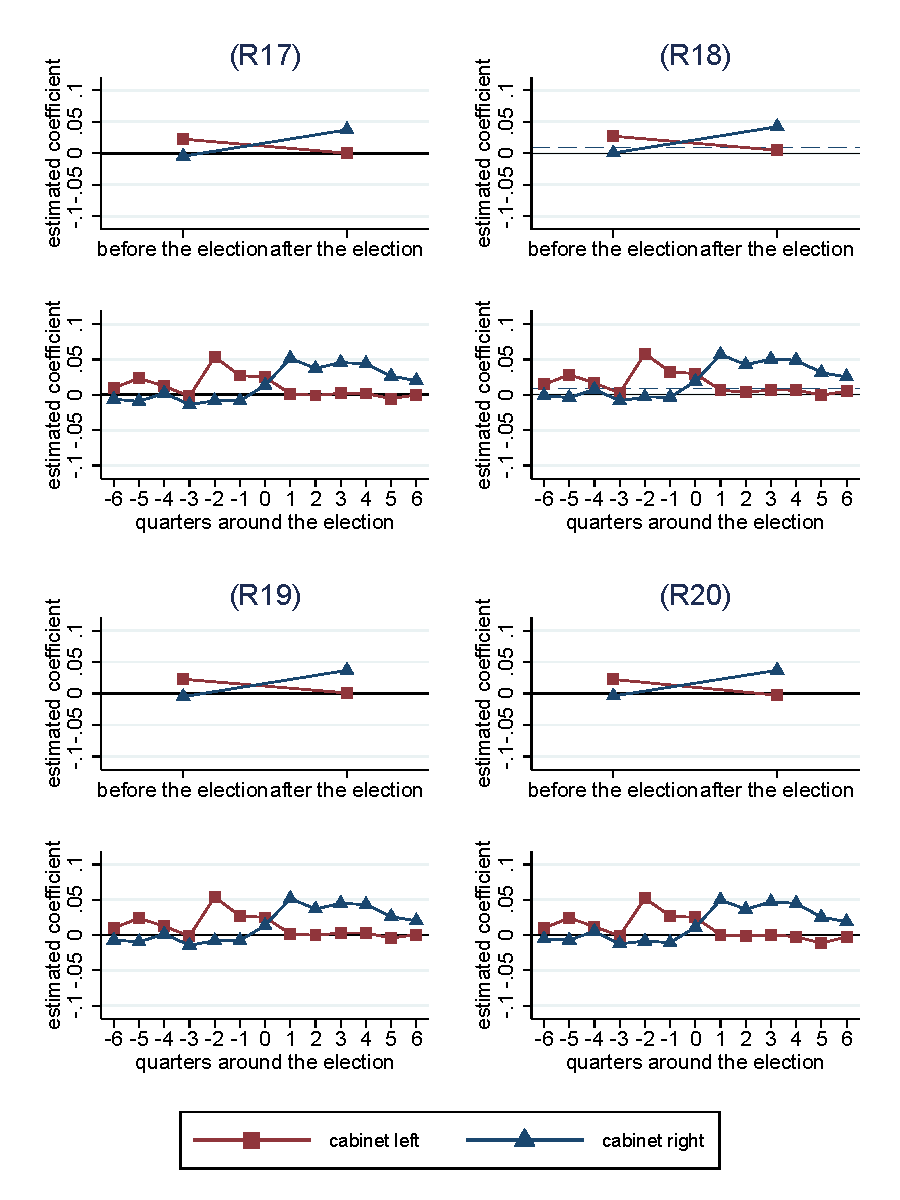
\includegraphics[width=1\textwidth]{../results/decisions/temporary_protection_rate_graphs_R17-R20.pdf}
	\scriptsize{Note: These figures show the time evolution of the share of temporary protection decisions in all decisions made in that quarter in fixed effects regression with a set of dummies for before and after the election or a set of dummies for different quarters before and after an election in a quarter t = 0. Significant coefficients are indicated by filled plot markers.}
\end{figure}

\begin{table}[htbp]\centering
\def\sym#1{\ifmmode^{#1}\else\(^{#1}\)\fi}
\caption{Coefficients quarterly model temporary\_protection\_rate R17 - R20}
\begin{tabular}{l*{8}{c}}
\hline\hline
                    &\multicolumn{1}{c}{(1)}&\multicolumn{1}{c}{(2)}&\multicolumn{1}{c}{(3)}&\multicolumn{1}{c}{(4)}&\multicolumn{1}{c}{(5)}&\multicolumn{1}{c}{(6)}&\multicolumn{1}{c}{(7)}&\multicolumn{1}{c}{(8)}\\
                    &\multicolumn{1}{c}{left\_R17}&\multicolumn{1}{c}{right\_R17}&\multicolumn{1}{c}{left\_R18}&\multicolumn{1}{c}{right\_R18}&\multicolumn{1}{c}{left\_R19}&\multicolumn{1}{c}{right\_R19}&\multicolumn{1}{c}{left\_R20}&\multicolumn{1}{c}{right\_R20}\\
\hline
 6 quarters before the election&     0.00977         &    -0.00624         &      0.0147         &     -0.0102         &      0.0102         &    -0.00707         &     0.00984         &    -0.00559         \\
                    &   (0.00770)         &   (0.00921)         &   (0.00837)         &   (0.00783)         &   (0.00778)         &   (0.00914)         &   (0.00767)         &   (0.00920)         \\
[1em]
 5 quarters before the election&      0.0235\sym{*}  &    -0.00919         &      0.0284\sym{**} &     -0.0132         &      0.0239\sym{*}  &    -0.00960         &      0.0243\sym{*}  &    -0.00704         \\
                    &    (0.0100)         &   (0.00732)         &   (0.00978)         &   (0.00686)         &    (0.0100)         &   (0.00730)         &    (0.0101)         &   (0.00738)         \\
[1em]
 4 quarters before the election&      0.0121         &     0.00249         &      0.0168         &    -0.00134         &      0.0125         &     0.00143         &      0.0119         &     0.00527         \\
                    &    (0.0110)         &   (0.00825)         &    (0.0107)         &   (0.00775)         &    (0.0110)         &   (0.00827)         &    (0.0109)         &   (0.00824)         \\
[1em]
 3 quarters before the election&    -0.00210         &     -0.0140         &     0.00248         &     -0.0177\sym{*}  &    -0.00144         &     -0.0144         &    -0.00105         &     -0.0124         \\
                    &   (0.00845)         &   (0.00747)         &   (0.00918)         &   (0.00723)         &   (0.00825)         &   (0.00754)         &   (0.00840)         &   (0.00760)         \\
[1em]
 2 quarters before the election&      0.0536\sym{***}&    -0.00832         &      0.0582\sym{***}&     -0.0122         &      0.0539\sym{***}&    -0.00809         &      0.0522\sym{***}&    -0.00843         \\
                    &   (0.00832)         &   (0.00929)         &   (0.00742)         &   (0.00927)         &   (0.00821)         &   (0.00930)         &   (0.00846)         &   (0.00917)         \\
[1em]
 1 quarters before the election&      0.0274\sym{***}&    -0.00865         &      0.0326\sym{***}&     -0.0125         &      0.0273\sym{***}&    -0.00761         &      0.0270\sym{***}&     -0.0106         \\
                    &   (0.00724)         &    (0.0116)         &   (0.00787)         &    (0.0111)         &   (0.00724)         &    (0.0115)         &   (0.00751)         &    (0.0113)         \\
[1em]
Quarter of the election&      0.0247\sym{**} &      0.0135         &      0.0300\sym{***}&     0.00979         &      0.0249\sym{**} &      0.0136         &      0.0250\sym{**} &      0.0109         \\
                    &   (0.00822)         &    (0.0120)         &   (0.00768)         &    (0.0126)         &   (0.00820)         &    (0.0119)         &   (0.00831)         &    (0.0119)         \\
[1em]
 1 quarters after the election&     0.00163         &      0.0517\sym{***}&     0.00660         &      0.0479\sym{**} &     0.00197         &      0.0517\sym{***}&    0.000507         &      0.0498\sym{***}\\
                    &   (0.00663)         &    (0.0148)         &   (0.00687)         &    (0.0146)         &   (0.00661)         &    (0.0149)         &   (0.00660)         &    (0.0148)         \\
[1em]
 2 quarters after the election&   -0.000952         &      0.0374\sym{*}  &     0.00359         &      0.0335\sym{*}  &   -0.000375         &      0.0369\sym{*}  &    -0.00159         &      0.0366\sym{*}  \\
                    &   (0.00647)         &    (0.0150)         &   (0.00758)         &    (0.0145)         &   (0.00640)         &    (0.0148)         &   (0.00616)         &    (0.0151)         \\
[1em]
 3 quarters after the election&     0.00220         &      0.0456\sym{***}&     0.00680         &      0.0414\sym{***}&     0.00317         &      0.0450\sym{***}&    0.000416         &      0.0470\sym{***}\\
                    &   (0.00535)         &    (0.0112)         &   (0.00664)         &    (0.0110)         &   (0.00545)         &    (0.0111)         &   (0.00523)         &    (0.0113)         \\
[1em]
 4 quarters after the election&     0.00186         &      0.0440\sym{***}&     0.00662         &      0.0399\sym{***}&     0.00281         &      0.0432\sym{***}&    -0.00231         &      0.0449\sym{***}\\
                    &   (0.00589)         &   (0.00975)         &   (0.00722)         &   (0.00981)         &   (0.00594)         &   (0.00948)         &   (0.00600)         &   (0.00981)         \\
[1em]
 5 quarters after the election&    -0.00534         &      0.0265\sym{*}  &   -0.000389         &      0.0223\sym{*}  &    -0.00412         &      0.0261\sym{*}  &     -0.0114         &      0.0255\sym{*}  \\
                    &   (0.00569)         &    (0.0105)         &   (0.00756)         &   (0.00987)         &   (0.00551)         &    (0.0104)         &   (0.00588)         &    (0.0106)         \\
[1em]
 6 quarters after the election&   -0.000215         &      0.0201\sym{*}  &     0.00495         &      0.0163         &    0.000485         &      0.0202\sym{*}  &    -0.00251         &      0.0189         \\
                    &   (0.00765)         &   (0.00974)         &   (0.00869)         &   (0.00902)         &   (0.00759)         &   (0.00976)         &   (0.00775)         &   (0.00969)         \\
\hline
Observations        &       12921         &       12921         &       12921         &       12921         &       12921         &       12921         &       12868         &       12868         \\
\hline\hline
\multicolumn{9}{l}{\footnotesize Standard errors in parentheses}\\
\multicolumn{9}{l}{\footnotesize \sym{*} \(p<0.05\), \sym{**} \(p<0.01\), \sym{***} \(p<0.001\)}\\
\end{tabular}
\end{table}



\end{document}